\documentclass[11pt]{book}

% Paquetes
\usepackage[spanish]{babel} % Configura el idioma en español
\usepackage[utf8]{inputenc} % Codificación de caracteres UTF-8
\usepackage[T1]{fontenc} % Codificación de fuente
\usepackage{amsmath,amsfonts,amssymb} % Paquetes para matemáticas
\usepackage{graphicx} % Para incluir gráficos
\usepackage{geometry} % Para configurar los márgenes
\usepackage[hidelinks]{hyperref} % Para enlaces hipertextuales sin colores
\usepackage{enumitem} % Para personalizar listas
\usepackage{cite}
\usepackage{graphicx}
\usepackage[utf8]{inputenc}
\usepackage[T1]{fontenc}
\usepackage[spanish]{babel} % Establece el idioma español
\usepackage{pgfplots}
\pgfplotsset{compat=1.16} % Puede que necesites ajustar la versión
\usepackage{csquotes} % Carga el paquete csquotes
\usepackage{graphicx} % Required for inserting images
\usepackage{listings}
\usepackage{xcolor}
\usepackage{hyperref}
\setlength{\parindent}{0.5in}
\usepackage{setspace}
\usepackage{amssymb}
\usepackage{amsthm}
\usepackage{minitoc}

\doublespacing
\renewcommand{\baselinestretch}{1.5}

\theoremstyle{plain}
\newtheorem{proposición}{proposición}[section]
\newtheorem{lema}[proposición]{Lema}
\newtheorem{teo}[proposición]{Teorema}
\newtheorem{coro}[proposición]{Corolario}
\newtheorem{obs}[proposición]{Observación}

\theoremstyle{definition}
\newtheorem{defi}[proposición]{definición}
\newtheorem{ejemplo}[proposición]{Ejemplo}

\newcommand{\Al}{(\mathcal{A},\mathds{F},\odot)}
\newcommand{\A}{\mathcal{A}}
\newcommand{\B}{\mathcal{B}}
\newcommand{\D}{\mathcal{D}}
\newcommand{\C}{\mathbb{C}}
\newcommand{\I}{\mathcal{I}}
\newcommand{\J}{\mathcal{J}}
\newcommand{\R}{\mathbb{R}}
\newcommand{\N}{\mathbb{N}}
\newcommand{\Z}{\mathbb{Z}}
\newcommand{\fu}{f:D\longrightarrow \mathds{R}}
\newcommand{\fun}{f:[a,b]\longrightarrow \mathds{R}}
\newcommand{\E}{\mathcal{E}}
\newcommand{\F}{\mathds{F}}
\newcommand{\op}{``}
\newcommand{\cl}{''}
\newcommand{\po}{^}
\newcommand{\Q}{\matbbb{Q}}
\newcommand{\U}{\mathcal{U}}


% Configuración de márgenes
\geometry{margin=1in}

% Título
\title{Notas para un Curso de Ecuaciones en Derivadas Parciales}
\author{Kevin Cárdenas}
\date{\today}

\begin{document}
\dominitoc 
\begin{titlepage}
    \centering
    \vspace{1cm}
    \Huge\textbf{Notas para un Curso Introductorio a las Ecuaciones en Derivadas Parciales}
    \vfill
    \begin{figure}[h]
        \centering
        
\includegraphics[width=0.2\textwidth]{logoudea.jpg}
    \end{figure}
    \vspace{1cm}
    \Large\textbf{Kevin Mateo Cárdenas Gallego}\\
    \large{Universidad de Antioquia}\\
    \large{Medellín, Colombia}\\
    \large{2023}
\end{titlepage}

\tableofcontents % Índice

\newpage

\chapter{Primeros Pasos}
\minitoc
En el estudio de fenómenos físicos y matemáticos, las Ecuaciones en Derivadas Parciales (EDP) desempeñan un papel fundamental. Son ecuaciones que involucran derivadas parciales de una o más variables independientes y, como resultado, modelan una amplia variedad de procesos en ciencias naturales, ingeniería y matemáticas.

\section{Definiciones}
\subsection*{Definición de una Ecuación en Derivadas Parciales}

Una Ecuación en Derivadas Parciales es una ecuación que relaciona una función desconocida de varias variables con sus derivadas parciales. Generalmente, se representa de la siguiente manera:

\begin{equation}
F(x_1, x_2, \ldots, x_n, u, \frac{\partial u}{\partial x_1}, \frac{\partial u}{\partial x_2}, \ldots, \frac{\partial u}{\partial x_n}, \frac{\partial^2 u}{\partial x_1^2}, \ldots) = 0.
\end{equation}

Donde $u$ es la función desconocida y las $x_i$ son las variables independientes.

\subsection*{Órdenes de las EDP}

Las Ecuaciones en Derivadas Parciales (EDP) se clasifican en función del orden de las derivadas parciales presentes en la ecuación. A continuación, se proporcionan ejemplos que ilustran los órdenes más comunes:

\begin{itemize}
    \item \textbf{Primer orden:} Las EDP de primer orden involucran únicamente derivadas de primer orden con respecto a las variables independientes. Un ejemplo de una EDP de primer orden es la ecuación de transporte:
    
    \begin{equation}
    \frac{\partial u}{\partial t} + c\frac{\partial u}{\partial x} = 0.
    \end{equation}
    
    Donde $u$ es la función desconocida y $c$ es una constante que representa la velocidad de transporte.

    \item \textbf{Segundo orden:} Las EDP de segundo orden involucran derivadas de segundo orden con respecto a las variables independientes. Un ejemplo clásico de una EDP de segundo orden es la ecuación del calor:
    
    \begin{equation}
    \frac{\partial u}{\partial t} = \alpha \frac{\partial^2 u}{\partial x^2}.
    \end{equation}
    
    Donde $u$ representa la temperatura en una barra, $t$ es el tiempo, $x$ es la posición, y $\alpha$ es la difusividad térmica.

    \item \textbf{Orden superior:} Las EDP de orden superior incluyen derivadas de orden superior (mayor que dos) con respecto a las variables independientes. Un ejemplo es la ecuación de Laplace, una EDP de orden superior que describe el potencial eléctrico en un campo electrostático:
    
    \begin{equation}
    \nabla^2 \phi = 0.
    \end{equation}
    
    Donde $\phi$ representa el potencial eléctrico y $\nabla^2$ es el operador laplaciano.
\end{itemize}

\subsection*{Tipos de EDP}

Las Ecuaciones en Derivadas Parciales (EDP) se clasifican en tres categorías principales según su forma general:

\begin{enumerate}
    \item \textbf{EDP Lineales:} Una EDP se considera lineal si se puede expresar de la siguiente manera:
    
    \begin{equation}
    \sum_{i=1}^{n} a_i(x) \frac{\partial^{m_i} u}{\partial x_i^{m_i}} + b(x)u = f(x).
    \end{equation}
    
    Donde $u$ es la función desconocida, $a_i(x)$, $b(x)$ y $f(x)$ son funciones dadas, y $m_i$ son enteros no negativos, $x  = (x_{1} , \ldots , x_{n})$. En las EDP lineales, todas las derivadas parciales están elevadas a la primera potencia y no se multiplican entre sí.
    
    \item \textbf{EDP Cuasilineales:} Las EDP cuasilineales permiten derivadas de orden superior y productos de derivadas, pero el término lineal prevalece. Se expresan de la siguiente manera:
    
    \begin{equation}
    \sum_{i=1}^{n} a_i(x, u) \prod_{j=1}^{n}\frac{\partial^{m_{i,j}}}{\partial x_{i,j}^{m_{i,j}}}(u) = b(x, u).
    \end{equation}
    
    Donde $u$ es la función desconocida, $a_i(x, u)$, $b(x, u)$ y son funciones dadas, y $m_{i,j}$ son enteros no negativos.
    
    \item \textbf{EDP Completamente No Lineales:} En las EDP completamente no lineales, los términos no lineales predominan y las derivadas pueden aparecer elevadas a potencias diferentes. Estas EDP se expresan de la siguiente manera:
    
    \begin{equation}
    F(x, u, \prod_{j=1}^{n}\frac{\partial^{m_{i,j}}}{\partial x_{i,j}^{m_{i,j}}}(u)) = 0.
    \end{equation}
    
    Donde $u$ es la función desconocida y $F(x, u, \frac{\partial^{m_{i,j}} u}{\partial x_{i,j}^{m_{i,j}}})$ es una función no lineal de las variables $u$, $x  = (x_{1} , \ldots , x_{n})$ y $\prod_{j=1}^{n}\frac{\partial^{m_{i,j}}}{\partial x_{i,j}^{m_{i,j}}}(u)$.
\end{enumerate}

\subsection*{Solución Particular y Solución General}

En el contexto de las EDP, es importante distinguir entre la solución particular y la solución general:

\begin{itemize}
    \item \textbf{Solución Particular:} Es una solución específica que satisface la EDP junto con las condiciones de contorno y condiciones iniciales especificadas para un problema particular.
    
    \item \textbf{Solución General:} Es una solución que satisface la EDP sin considerar condiciones específicas. La solución general incluye todas las posibles soluciones particulares y puede contener constantes arbitrarias.
\end{itemize}

El estudio de EDP implica encontrar soluciones particulares que se adapten a problemas específicos y, en algunos casos, encontrar la solución general que describe todas las posibles soluciones del problema.

\newpage
\section{Método de Resolución para EDP Lineales de Primer Orden}

Consideremos la siguiente ecuación diferencial parcial lineal de primer orden en dos variables:

\setcounter{equation}{0}
\begin{equation}
a(x, y) \frac{\partial u}{\partial x} + b(x, y) \frac{\partial u}{\partial y} = c(x, y) u + d(x,y).
\end{equation}

Para resolver esta ecuación, podemos usar el método de cambio de variable.

\subsection*{Paso 1: Cambio de Variable}

\begin{equation}
\frac{dy}{dx} = -\frac{a(x, y)}{b(x, y)}.
\end{equation}

De esta EDO, encontramos la curva solución $\eta(x, y)$, que relaciona $x$ y $y$.

\begin{equation}
\frac{d}{dx} \left( b(x, y) u \right) = c(x, y) u + d(x,y).
\end{equation}

\subsection*{Paso 2: Definición de Nueva Variable}

Definimos una nueva variable $\xi(x, y)$ como $\xi(x, y) = y$. Suponiendo que $\frac{\partial u}{\partial x} \neq 0$, para que el jacobiano de la transformación no sea nulo.

\subsection*{Paso 3: Reemplazo en la EDP Original}
Reemplazamos $\frac{\partial u}{\partial x}$ y $\frac{\partial u}{\partial y}$ en la EDP original con las derivadas de $\eta$ y $\psi$ respecto a $x$ y $y$, respectivamente (suponiendo $W(\eta(x,y),\psi(x,y)) = u(x,y)$):

\begin{align}
\frac{\partial u}{\partial x} &= \frac{d\eta}{dx}\frac{\partial W}{\partial \eta} + \frac{d\psi}{dx}\frac{\partial W}{\partial \psi} \\
\frac{\partial u}{\partial y} &= \frac{d\eta}{dy}\frac{\partial W}{\partial \eta} + \frac{d\psi}{dy}\frac{\partial W}{\partial \psi}.
\end{align}

\subsection*{Paso 4: Sustitución en la EDP}
Sustituimos estas expresiones en la EDP original:

\begin{align}
a(x, y) \left(\frac{d\eta}{dx}\frac{\partial W}{\partial \eta} + \frac{d\psi}{dx}\frac{\partial W}{\partial \psi}\right) + b(x, y) \left(\frac{d\eta}{dy}\frac{\partial W}{\partial \eta} + \frac{d\psi}{dy}\frac{\partial W}{\partial \psi}\right) &= c(x, y) W + d(x,y).
\end{align}

Simplificamos la ecuación y agrupamos términos que contengan $\frac{\partial W}{\partial \eta}$ y $\frac{\partial W}{\partial \psi}$:

\begin{align}
\left[a(x, y)\frac{d\eta}{dx} + b(x, y)\frac{d\eta}{dy}\right]\frac{\partial W}{\partial \eta} + \left[a(x, y)\frac{d\xi}{dx} + b(x, y)\frac{d\xi}{dy}\right]\frac{\partial W}{\partial \xi} = c(x, y)W + d(x, y).
\end{align}

Donde $\left[a(x, y)\frac{d\eta}{dx} + b(x, y)\frac{d\eta}{dy}\right]\frac{\partial W}{\partial \eta} = 0$, pues
$a(x, y)\frac{d\eta}{dx} + b(x, y)\frac{d\eta}{dy} = 0$, por (2).

Luego la EDP, queda como una EDO lineal:

\begin{align}
\left[a(x, y)\frac{d\xi}{dx} + b(x, y)\frac{d\xi}{dy}\right]\frac{\partial W}{\partial \xi} = c(x, y)W + d(x, y).
\end{align}

\subsection*{Paso 5: solución de la EDO lineal}
la solución general será:

\begin{align}
W(\xi , \eta) = \frac{1}{e ^{\int -c(x(\xi , \eta), y(\xi , \eta))d\xi}} \left(\int d(x(\xi , \eta), y(\xi , \eta)) e ^{\int -c(x(\xi , \eta), y(\xi , \eta))d\xi} \, d\xi + G(\eta)\right).
\end{align}

donde $W(\xi , \eta) = u(x(\xi , \eta), y(\xi , \eta))$

\subsection*{Paso 6: Reemplazar de vuelta}
Como la sustitución tenia jacobiano no nulo, se puede reemplazar de vuelta, por lo que existe una transformación $\xi(x, y) , \eta(x,y)$ inversa de la transformación inicial, y así queda la solución general dada por:
\begin{align}
    u(x, y) = W(\xi(x, y) , \eta(x, y)).
\end{align}

\newpage
\section{Metodo de Lagrange}
Consideremos la siguiente ecuación diferencial parcial cuasilineal de primer orden en dos variables:

\setcounter{equation}{0}
\begin{equation}
a(x, y, u) \frac{\partial u}{\partial x} + b(x, y, u) \frac{\partial u}{\partial y} = c(x, y, u).
\end{equation}

considere el siguiente sistema, llamado el sistema subsidiario:

\begin{align}
    \frac{dx}{a(x,y,u)} = \frac{dy}{b(x,y,u)} = \frac{du}{c(x,y,u)}.
\end{align}

Si $a \neq 0$, entonces las ecuaciones subsidiarias son equivalentes al sistema:
\begin{align}
     \frac{dy}{dx} = \frac{b(x,y,u)}{a(x,y,u)}, \hspace{8mm} 
     \frac{du}{dx} = \frac{c(x,y,u)}{a(x,y,u)}
\end{align}

La ventaja del sistema subsidiario es que evita la distinción entre variables dependientes y variables independientes. 

Resolviendo el sistema subsidiario (en (3) por ejemplo) obtenemos dos curvas características. Que serán curvas integrales de las ecuaciones subsidiarias.

Por ejemplo:

\begin{align}
     \phi(x,y,u) \hspace{4mm}de\hspace{4mm} \frac{dy}{dx} = \frac{b(x,y,u)}{a(x,y,u)}.
\end{align}
y 
\begin{align}
     \psi(x,y,u) \hspace{4mm}de\hspace{4mm}  \frac{du}{dx} = \frac{c(x,y,u)}{a(x,y,u)}.
\end{align}
$\phi(x,y,u)$ y $\psi(x,y,u)$ son las constantes arbitrarias que surgen de la solución de la EDO, si estas son funcionalmente independientes en alguna región en el espacio $xyz$, entonces la solución general de la ecuación cuasi lineal viene dada por:

\begin{align}
    F(\phi,\psi) = 0
\end{align}

donde F es una función arbitraria. O manera equivalente, a partir del teorema de la función implícita:

\begin{align}
    \phi = g(\psi) \hspace{4mm}o\hspace{4mm} \psi = f(\phi)
\end{align}

donde $f$ y $g$ son funciones arbitrarias.

\subsection{El método de los multiplicadores}
Una técnica útil en la solución de ecuaciones es el método de los multiplicadores.

\begin{proposición}
Si $\frac{a}{b} = \frac{c}{d}$, entonces
$$\frac{\lambda a + \beta c}{\lambda b + \beta d} = \frac{a}{b} = \frac{c}{d}$$
Para $\lambda, \beta$ arbitrarios
\end{proposición}

\begin{obs}
    Aplicando la proposición anterior al sistema subsidiario 
    
    $$\frac{dx}{a(x,y,u)} = \frac{dy}{b(x,y,u)} = \frac{du}{c(x,y,u)}.$$
    
    obtenemos
    
    $$\frac{\lambda dx + \mu dy + \beta du}{\lambda a(x,y,u) + \mu b(x,y,u) + \beta c(x,y,u)} =\frac{dx}{a(x,y,u)} = \frac{dy}{b(x,y,u)} = \frac{du}{c(x,y,u)}.$$

    De esta forma podemos obtener algunas ecuaciones diferenciales relacionadas mas fáciles de integrar.

    En particular, si $\lambda, \mu, \beta$ se eligen de tal manera que:
    $$\lambda a(x,y,u) + \mu b(x,y,u) + \beta c(x,y,u) = 0,$$

    entonces, si existe una función $v$ tal que:
    $$dv = \lambda dx + \mu dy + \beta du$$

    $v(x,y,u)$ es una curva integral de las ecuaciones subsidiarias.
\end{obs}

\newpage
\section{Método de las Características para EDP Cuasilineales con Condición Inicial}

Supongamos que tenemos la siguiente Ecuación en Derivadas Parciales (EDP) cuasilineal de primer orden, junto con una condición inicial, sobre una curva
\setcounter{equation}{0}
\begin{align}
    a(x, y, u) \frac{\partial u}{\partial x} + b(x, y, u) \frac{\partial u}{\partial y} = c(x, y, u)\\
    u|_{\gamma} = u_0(s)\\
    \gamma =\{(x_0(s),y_0(s))\}
\end{align}

Basta resolver el siguiente sistema simultaneamente:
\begin{align}
    \frac{dx}{dt} = a(x,y,u) \hspace{32mm} x(0) = x_o(s)\\
    \frac{dy}{dt} = b(x,y,u) \hspace{32mm} y(0) = y_o(s)\\
    \frac{du}{dt} = a(x,y,u) \hspace{32mm} u(0) = u_o(s)
\end{align}
Luego, debemos dejar a $u$ en términos de $x$ e $y$.

\subsection*{Perdida de unicidad de la solución}
Note que  (1) se puede ver como el siguiente producto punto:

\begin{align}
    (a,b,c)\cdot(\frac{\partial u}{\partial x}, \frac{\partial u}{\partial y}, -1)
\end{align}
Y si tenemos una solución $u(x,y)$, esta ecuación expresa que el campo
$$(x,y) \to (a(x,y,u(x,y)),b(x,y,u(x,y)),c(x,y,u(x,y))).$$ 
es tangente a la superficie dada por $u$. Donde $(\frac{\partial u}{\partial x}, \frac{\partial u}{\partial y}, -1)$ es justamente normal.

Ahora bien, si
\begin{align}
det
    \begin{pmatrix}
        a(x,y,u)|_{\gamma} & a(x,y,u)|_{\gamma} \\
        \frac{d x_0(s)}{ds} & \frac{d y_0(s)}{ds}
    \end{pmatrix}
    \neq 0
\end{align}
Que es la \emph{condición de transversabilidad}, entonces \emph{el sistema tiene una única solución}

Por otra parte 
\begin{align}
    \begin{pmatrix}
        a(x,y,u)|_{\gamma} \\ a(x,y,u)|_{\gamma} \\ c(x,y,u)|_{\gamma}
    \end{pmatrix}
    =
    \alpha \begin{pmatrix}
        \frac{d x_0(s)}{ds} \\ \frac{d y_0(s)}{ds} \\ \frac{d u_0(s)}{ds}
    \end{pmatrix}
\end{align}
Para algún $s_0$ que es la \emph{condición de colinealidad}, entonces \emph{el sistema tiene una infinitas soluciones}. Ciertamente porque si cambiamos la curva inicial por una curva $\beta = \{(\overline{x_0(\theta)},\overline{y_0(\theta)})\}$ tal que la curva pase por $\gamma(s_0)$ para un $\theta_0$ y $u_0(s_0) = \overline{u_0(\theta_0)}$, entonces la solución del sistema 
\begin{align}
    a(x, y, u) \frac{\partial u}{\partial x} + b(x, y, u) \frac{\partial u}{\partial y} = c(x, y, u)\\
    u|_{\beta} = \overline{u_0(\theta)}\\
    \beta =\{(\overline{x_0(\theta)},\overline{y_0(\theta)})\}
\end{align}

También cumple que:
\begin{align}
    u|_{\gamma} = u_0(s)\\
    \gamma =\{(x_0(s),y_0(s))\}
\end{align}

Ahora bien, si no se cumple la \emph{condición de transversabilidad} y tampoco hay \emph{colinealidad} entonces \emph{no existe solución} al problema de Cauchy.

\section{Ecuación Eikonal}
La ecuación Eikonal es de la forma:
\setcounter{equation}{0}
\begin{align}
    \frac{\partial u}{\partial x}^{2} + \frac{\partial u}{\partial y}^{2} = \nu ^{2}
\end{align}

Al escribir las ecuaciones características queda:
\begin{align}
    (\frac{\partial u}{\partial x}, \frac{\partial u}{\partial y}, \nu^{2})\cdot(\frac{\partial u}{\partial x},\frac{\partial u}{\partial y},-1) = 0
\end{align}

Este vector $(\frac{\partial u}{\partial x}, \frac{\partial u}{\partial}, \nu^{2})$ describe una dirección tangente a la superficie solución. 

Tenemos el sistema:

\begin{align}
    \frac{dx}{dt} = \frac{\partial u}{\partial x}, \hspace{8mm} \frac{dy}{dt} = \frac{\partial u}{\partial y}, \hspace{8mm}\frac{du}{dt} = \nu^{2}
\end{align}

Podemos calcular
\begin{align*}
    \frac{d^{2}x}{dt^{2}} &= \frac{d}{dt}(\frac{\partial u}{\partial x}) = \frac{\partial^{2} u}{\partial x^{2}}\frac{dx}{dt} + \frac{\partial^{2} u}{\partial x \partial y}\frac{dy}{dt}\\
    &= \frac{1}{2}\frac{\partial (\frac{\partial u}{\partial x} ^{2} + \frac{\partial u}{\partial y} ^{2})}{\partial x} \\
    &= \frac{1}{2} \frac{\partial \nu^{2}(x,y)}{\partial x}
\end{align*}
Y similar:
\begin{align*}
    \frac{d^{2}y}{dt^{2}} = \frac{1}{2} \frac{\partial \nu(x,y)}{\partial y}
\end{align*}

Por lo tanto.
\begin{align*}
    \frac{du}{dt} = \frac{\partial u}{\partial x} ^{2} + \frac{\partial u}{\partial y} ^{2} = \nu^{2}(x,y)
\end{align*}
Integrando la ultima ecuación tenemos que:
\begin{align}
    u(x(t), y(t)) = u(x(0), y(0)) + \int_{0}^{t} \nu^{2}(x(\tau), y(\tau)) d\tau,
\end{align}

\section{Resolución de EDP Completamente No Lineal de Primer Orden con Condiciones Iniciales}

Dada la EDP completamente no lineal, junto con una condición inicial:

\setcounter{equation}{0}
\begin{align}
    F(x, y, u, \frac{\partial u}{\partial x}, \frac{\partial u}{\partial y}) = 0 \\
    u(x_0(s), y_0(s)) = u_0(s)
\end{align}

donde \(u(x_0(s), y_0(s))\) es una curva en el dominio y \(u_0(s)\) es el valor inicial de \(u\) en esa curva.

Vamos a considerar las siguientes variables auxiliares:
\begin{align}
    p = \frac{\partial u}{\partial x} \hspace{16mm} q = \frac{\partial u}{\partial y}
\end{align}

Resolvemos las siguentes ecuaciones, llamadas \emph{condición de transversabilidad generalizada}
\begin{align}
    F(x, y, u, p_0, q_0) = 0 \\
    \begin{pmatrix}
        p_0 \\ q_0 \\ -1
    \end{pmatrix}
    \cdot
    \begin{pmatrix}
        \frac{d x_0(s)}{ds} \\ \frac{d y_0(s)}{ds} \\ \frac{d u_0(s)}{ds}
    \end{pmatrix} = 0 \\
    \frac{d x_0}{ds}\frac{d F}{dq} - \frac{d y_0}{ds}\frac{d F}{dp} \neq 0
\end{align}

hallando $p_0(s)$ y $q_0(s)$ que seran las condiciones iniciales del siguiente sistema:
\begin{align}
    \frac{dx}{dt} &= \frac{dF}{p} \hspace{50mm} x(0) = x_o(s)\\
    \frac{dy}{dt} &= \frac{dF}{q} \hspace{50mm} y(0) = y_o(s)\\
    \frac{dp}{dt} &= -p(\frac{dF}{u} + \frac{dF}{x}) \hspace{32mm} p(0) = p_o(s)\\
    \frac{dq}{dt} &= -q(\frac{dF}{q} + \frac{dF}{y}) \hspace{32mm} q(0) = q_o(s)\\
    \frac{du}{dt} &= p\frac{dF}{dp} + q\frac{dF}{dq} \hspace{36mm} u(0) = u_o(s)
\end{align}

Si el sistema de la condición de transversabilidad generalizado podría arrojar más de una solución $p_0(s), q_0(s)$, con cada una se puede resolver el problema de Cauchy y serán soluciones validas.

Lo otro es que la condición de transversabilidad (6) aquí viene dada por los vectores $(F_p,F_q)$ y $(\frac{dx_0}{ds},\frac{dy_0(s)}{ds})$.

\begin{obs}
Note que el caso no lineal analiza el caso general, lineal, cuasilineal, y completamente no lineal. Y el analisis de perdida de unicidad en función de las condición de transversabilidad es equivalente.
\end{obs}

\section{Ecuaciones de Segundo Orden Cuasilineales y su Clasificación}

Las ecuaciones diferenciales parciales (EDP) de segundo orden cuasilineales son una clase importante de EDPs que involucran derivadas de segundo orden (segundas derivadas) de una función desconocida $u(x, y)$. La forma general de una EDP cuasilineal de segundo orden es:

\begin{equation}
a(x, y, u) \frac{\partial^2 u}{\partial x^2} + 2b(x, y, u) \frac{\partial^2 u}{\partial x \partial y} + c(x, y, u) \frac{\partial^2 u}{\partial y^2} = d(x, y, u, \frac{\partial u}{\partial x}, \frac{\partial u}{\partial y})
\end{equation}

Donde $a(x, y, u)$, $b(x, y, u)$, $c(x, y, u)$ y $d(x, y, u, \frac{\partial u}{\partial x}, \frac{\partial u}{\partial y})$ son funciones conocidas que dependen de $x$, $y$, $u$, y posiblemente de las derivadas parciales de $u$.


Para simplificar esta ecuación, realizamos un cambio de variable introduciendo dos nuevas variables, $\xi$ y $\eta$, de la siguiente manera:

\[
u(x, y) = W(\xi, \eta)
.\]

Donde:

\[
\xi = \xi(x, y)
.\]

\[
\eta = \eta(x, y)
.\]

Ahora, calculemos las derivadas parciales de $u$ con respecto a $x$ y $y$ en términos de $\xi$ y $\eta$:

\[
\frac{\partial u}{\partial x} = \frac{\partial W}{\partial \xi} \frac{\partial \xi}{\partial x} + \frac{\partial W}{\partial \eta} \frac{\partial \eta}{\partial x}
.\]

\[
\frac{\partial u}{\partial y} = \frac{\partial W}{\partial \xi} \frac{\partial \xi}{\partial y} + \frac{\partial W}{\partial \eta} \frac{\partial \eta}{\partial y}
.\]

Ahora, calculemos las segundas derivadas de $u$ con respecto a $x$ y $y$ utilizando las expresiones anteriores:

\[
\frac{\partial^2 u}{\partial x^2} = \frac{\partial}{\partial x}\left(\frac{\partial u}{\partial x}\right) = \frac{\partial}{\partial x}\left(\frac{\partial W}{\partial \xi} \frac{\partial \xi}{\partial x} + \frac{\partial W}{\partial \eta} \frac{\partial \eta}{\partial x}\right)
.\]

\[
\frac{\partial^2 u}{\partial x \partial y} = \frac{\partial}{\partial x}\left(\frac{\partial u}{\partial y}\right) = \frac{\partial}{\partial x}\left(\frac{\partial W}{\partial \xi} \frac{\partial \xi}{\partial y} + \frac{\partial W}{\partial \eta} \frac{\partial \eta}{\partial y}\right)
.\]

\[
\frac{\partial^2 u}{\partial y^2} = \frac{\partial}{\partial y}\left(\frac{\partial u}{\partial y}\right) = \frac{\partial}{\partial y}\left(\frac{\partial W}{\partial \xi} \frac{\partial \xi}{\partial y} + \frac{\partial W}{\partial \eta} \frac{\partial \eta}{\partial y}\right)
.\]

Luego, sustituimos estas expresiones en la ecuación original:
\[
A(x, y, W) \frac{\partial^2 W}{\partial \xi^2} + 2B(x, y, W) \frac{\partial^2 W}{\partial \xi \partial \eta} + C(x, y, W) \frac{\partial^2 W}{\partial \eta^2} = D(x, y, W, P, Q)
.\]
donde:
\begin{align*}
A(x, y, W) &= a(x, y, W) \left(\frac{\partial \xi}{\partial x} \right)^2 + 2b(x, y, W) \left(\frac{\partial \xi}{\partial x} \frac{\partial \xi}{\partial y}\right) + c(x, y, W) \left(\frac{\partial \xi}{\partial y} \right)^2 \\
B(x, y, W) &= a(x, y, W) \frac{\partial \xi}{\partial x} \frac{\partial \eta}{\partial x} + b(x, y, W)\left(\frac{\partial \xi}{\partial y}  \frac{\partial \eta}{\partial x} + \frac{\partial \xi}{\partial x}  \frac{\partial \eta}{\partial y} \right) \ + c(x, y, W) \frac{\partial \eta}{\partial y} \frac{\partial \xi}{\partial y}\\
C(x, y, W) &= a(x, y, W) \left(\frac{\partial \eta}{\partial x} \right)^2 + 2b(x, y, W) \left(\frac{\partial \eta}{\partial x} \frac{\partial \eta}{\partial y}\right) + c(x, y, W) \left(\frac{\partial \eta}{\partial y} \right)^2 \\
\end{align*}
Estas EDPs cuasilineales pueden clasificarse en tres categorías principales según su comportamiento característico:

\subsection{Ecuaciones Elipticas}

\setcounter{equation}{0}
\begin{equation}
a(x, y, u) \frac{\partial^2 u}{\partial x^2} + 2b(x, y, u) \frac{\partial^2 u}{\partial x \partial y} + c(x, y, u) \frac{\partial^2 u}{\partial y^2} = d(x, y, u, \frac{\partial u}{\partial x}, \frac{\partial u}{\partial y})
\end{equation}

Una ecuación de segundo orden se considera \textbf{elíptica} en un punto $(x_0, y_0)$ si la matriz:

\[
\begin{pmatrix}
a(x_0, y_0, u) & b(x_0, y_0, u) \\
b(x_0, y_0, u) & c(x_0, y_0, u)
\end{pmatrix}
.\]
es definida positiva en ese punto. Matemáticamente, esto se expresa como:

\[
\det
\begin{vmatrix}
a(x_0, y_0, u) & b(x_0, y_0, u) \\
b(x_0, y_0, u) & c(x_0, y_0, u)
\end{vmatrix}
= a(x_0, y_0, u) \cdot c(x_0, y_0, u) - b^2(x_0, y_0, u) > 0
.\]

Para que la ecuación sea elíptica, el determinante de la matriz debe ser positivo en cada punto $(x_0, y_0)$ de interés.

Una ecuación elíptica en forma canónica es de la forma:

\[
\Delta W = f(x, y, W)
.\]

donde $\Delta$ es el operador laplaciano 

$$\Delta = \frac{\partial^2}{\partial x^2} + \frac{\partial^2}{\partial y^2}$$

Para llevar la ecuación original a esta forma, podemos hacer el siguiente cambio de variable:

\begin{align}
    \xi \hspace{8mm}de\hspace{8mm} \frac{dx}{dy} &= \frac{b}{a} \\
    \eta \hspace{8mm}de\hspace{8mm} \frac{dx}{dy} &= \frac{\sqrt{ac-b^{2}}}{a}
\end{align}
\subsection{Ecuaciones Parabólicas}
\setcounter{equation}{0}
\begin{equation}
a(x, y, u) \frac{\partial^2 u}{\partial x^2} + 2 b(x, y, u) \frac{\partial^2 u}{\partial x \partial y} + c(x, y, u) \frac{\partial^2 u}{\partial y^2} = d(x, y, u, \frac{\partial u}{\partial x}, \frac{\partial u}{\partial y})
\end{equation}
Una EDP de segundo orden se considera \textbf{parabólica} en un punto $(x_0, y_0)$ si la matriz:

\[
\begin{pmatrix}
a(x_0, y_0, u) & b(x_0, y_0, u) \\
b(x_0, y_0, u) & c(x_0, y_0, u)
\end{pmatrix}
.\]
Es decir:
\[
\det
\begin{vmatrix}
a(x_0, y_0, u) & b(x_0, y_0, u) \\
b(x_0, y_0, u) & c(x_0, y_0, u)
\end{vmatrix}
= a(x_0, y_0, u) \cdot c(x_0, y_0, u) - b^2(x_0, y_0, u) = 0
.\]

es singular en ese punto. Estas ecuaciones a menudo están asociadas con problemas de propagación de ondas y difusión en el tiempo, como la ecuación del calor o la ecuación de onda.

La forma canónica de una EDP parabólica es:
$$A u_{xx} + d(x, y, u, \frac{\partial u}{\partial x}, \frac{\partial u}{\partial y}) = 0$$

Para llevar la ecuación original a su forma canónica, podemos hacer el siguiente cambio de variable:

\begin{align}
    &\eta \hspace{8mm}de\hspace{8mm} \frac{dx}{dy} = \frac{b}{a} \\
    &\xi \hspace{8mm}tq\hspace{8mm} \frac{\partial(\eta, \xi)}{\partial(x,y)} \neq 0
\end{align}
\subsection{Ecuaciones Hiperbólicas}
\setcounter{equation}{0}
\begin{equation}
a(x, y, u) \frac{\partial^2 u}{\partial x^2} + 2 b(x, y, u) \frac{\partial^2 u}{\partial x \partial y} + c(x, y, u) \frac{\partial^2 u}{\partial y^2} = d(x, y, u, \frac{\partial u}{\partial x}, \frac{\partial u}{\partial y})
\end{equation}
Una EDP de segundo orden se considera \textbf{hiperbólica} en un punto $(x_0, y_0)$ si 
\[
\det
\begin{vmatrix}
a(x_0, y_0, u) & b(x_0, y_0, u) \\
b(x_0, y_0, u) & c(x_0, y_0, u)
\end{vmatrix}
= a(x_0, y_0, u) \cdot c(x_0, y_0, u) - b^2(x_0, y_0, u) < 0
.\]
La forma canonica de una EDP Hierbolica es:
$$A u_{xy} + d(x, y, u, \frac{\partial u}{\partial x}, \frac{\partial u}{\partial y}) = 0$$

Para llevar la ecuación original a su forma canónica, podemos hacer el siguiente cambio de variable:

\begin{align}
    \xi \hspace{8mm}de\hspace{8mm} \frac{dx}{dy} &= \frac{b - \sqrt{ac-b^{2}}}{a} \\
    \eta \hspace{8mm}de\hspace{8mm} \frac{dx}{dy} &= \frac{b + \sqrt{ac-b^{2}}}{a}
\end{align}

\newpage
\chapter{Ecuación de onda}
\minitoc
La ecuación de onda describe la propagación de ondas a través de un medio. Es fundamental en física y se utiliza para describir fenómenos como las ondas sonoras, las ondas de luz y las ondas en cuerdas o membranas.

La forma unidimensional de la ecuación de onda es:
\setcounter{equation}{0}
\begin{equation}
\frac{\partial^2 u}{\partial t^2} = c^2 \frac{\partial^2 u}{\partial x^2} + F(x,t)
\end{equation}

Donde:

\begin{itemize}
    \item \( u \) es el desplazamiento de la onda en función del tiempo \( t \) y de la posición \( x \).
    \item \( c \) es la velocidad de propagación de la onda en el medio.
\end{itemize}

\section{Solución General de la ecuación homogénea}
Note que la ecuación de onda homogénea es:
\begin{equation}
(\frac{\partial}{\partial t} - c \frac{\partial}{\partial x})(\frac{\partial}{\partial t} + c \frac{\partial}{\partial x}) u = 0
\end{equation}
De donde sabemos que las curvas características de la ecuación son:
\begin{equation*}
    \xi = x-ct \hspace{8mm} \eta = x+ct
\end{equation*}
A partir de la regla de la cadena:
\begin{align*}
    \frac{\partial u}{\partial x} &=  \frac{\partial u}{\partial \xi} \frac{\partial \xi}{\partial x} + \frac{\partial u}{\partial \eta} \frac{\partial \eta}{\partial x}\\
    &= \frac{\partial u}{\partial \xi} + \frac{\partial u}{\partial \eta}\\
    \frac{\partial^{2} u}{\partial x^{2}} &=\frac{\partial}{\partial x} \left( \frac{\partial u}{\partial \xi} + \frac{\partial u}{\partial \eta} \right) \\
    &= \frac{\partial^{2} u}{\partial \xi^{2}}\frac{\partial \xi}{\partial x} + \frac{\partial^{2} u}{\partial \xi \partial \eta}\frac{\partial \eta}{\partial x} + \frac{\partial^{2} u}{\partial \eta^{2}}\frac{\partial \eta}{\partial x} + \frac{\partial^{2} u}{\partial \eta \partial \xi}\frac{\partial \xi}{\partial x}\\
    &= \frac{\partial^{2} u}{\partial \xi^{2}} + 2\frac{\partial^{2} u}{\partial \eta \partial \xi} + \frac{\partial^{2} u}{\partial \eta^{2}}
\end{align*}
Además
\begin{align*}
    \frac{\partial u}{\partial t} &= \frac{\partial u}{\partial \xi} \frac{\partial \xi}{\partial t} + \frac{\partial u}{\partial \eta} \frac{\partial \eta}{\partial t} \\
    &= -c \frac{\partial u}{\partial \xi} + c \frac{\partial u}{\partial \eta}\\
    \frac{\partial u^{2}}{\partial t^{2}} &= \frac{\partial}{\partial t} \left(  -c \frac{\partial u}{\partial \xi} + c \frac{\partial u}{\partial \eta} \right) \\
    &= -c\left(\frac{\partial^{2} u}{\partial \xi^{2}}\frac{\partial \xi}{\partial t} + \frac{\partial^{2} u}{\partial \xi \partial \eta}\frac{\partial \eta}{\partial t} \right) +c \left(\frac{\partial^{2} u}{\partial \eta^{2}}\frac{\partial \eta}{\partial t} + \frac{\partial^{2} u}{\partial \xi \partial \eta}\frac{\partial \xi}{\partial t} \right)\\
    &= c^{2}\frac{\partial^{2} u}{\partial \xi^{2}} - 2c^{2}\frac{\partial^{2} u}{\partial \eta \partial \xi} + c^{2}\frac{\partial^{2} u}{\partial \eta^{2}}
\end{align*}

Entonces
\begin{align*}
    \frac{\partial^2 u}{\partial t^2} - c^2 \frac{\partial^2 u}{\partial x^2} &= 0\\ 
    4c^{2}\frac{\partial^{2} u}{\partial \eta \partial \xi} & = 0\\ 
    \frac{\partial^{2} u}{\partial \eta \partial \xi} & = 0
\end{align*}
Integrando tenemos:
\begin{align*}
    \frac{\partial^{2} u}{\partial \xi \partial \eta } & = 0\\
    \frac{\partial u}{\partial \eta} & = w(\eta)\\
    u(\xi,\eta) &= \int  w(\eta)d\eta + F(\xi)\\
\end{align*}
Y así
\begin{align}
    u(x,t) = F(x-ct) + G(x+ct)
\end{align}
Es la solución general a la ecuación de onda homogénea. Donde $F$ y $G$ son de clase $C^{1}$.

\newpage
\section{Fórmula de D'Alambert para el Problema de Cauchy}
Dado el problema de Cauchy para la ecuación de onda:

\begin{align*}
    \frac{\partial^2 u}{\partial t^2} &= c^2 \frac{\partial^2 u}{\partial x^2} \hspace{8mm} -\infty < x < \infty, \hspace{4mm} t > 0\\ 
    u(x,0)&= \varphi(x) \\
    \frac{\partial u}{\partial t}(x,0) &= \psi(x) \\
\end{align*}

Vimos que la solución general de la ecuación tiene la forma:
\[
    u(x,t) = F(x-ct) + G(x+ct)
.\]
La idea es tomar $F$ y $G$ que generen una solución que satisfaga las condiciones iniciales. Luego

\setcounter{equation}{0}
\begin{align}
    u(x,0) &= F(x) + G(x) = \varphi(x)\\
    \frac{\partial u}{\partial t}(x,0) &= -cF'(x) + cG'(x) = \psi(x)
\end{align}
Integrando en la última igualdad obtenemos
\[
 -F(x) + G(x) = \frac{1}{c}\int_{0}^{x}\psi(s)ds - F(0) + G(0)
.\]
Sumando con (4) obtenemos
\begin{align*}
    2G(x) &= \varphi(x) + \frac{1}{c}\int_{0}^{x}\psi(s)ds - F(0) + G(0)\\
    G(x) &= \frac{1}{2} \varphi(x) + \frac{1}{2c}\int_{0}^{x}\psi(s)ds - \frac{1}{2}F(0) + \frac{1}{2}G(0)
\end{align*}
y de nuevo en la ecuación (4) obtenemos
\begin{align*}
    F(x) &= \varphi(x) - G(x)\\
    &= \frac{1}{2} \varphi(x) - \frac{1}{2c}\int_{0}^{x}\psi(s)ds + \frac{1}{2}F(0) - \frac{1}{2}G(0)
\end{align*}
Finalmente obtenemos que
\begin{align}
    u(x,t) &= \frac{1}{2}\left( \varphi(x +ct) + \varphi(x -ct)\right) +\frac{1}{2c}\int_{x-ct}^{x+ct}\psi(s)ds
\end{align}
Esta la fórmula de d'Alambert para el problema de Cauchy para la ecuación de onda en la linea real.

\begin{teo}[Dependencia continua del dato inicial]
    Dado el problema de Cauchy.
    \begin{align*}
    \frac{\partial^2 u}{\partial t^2} &= c^2 \frac{\partial^2 u}{\partial x^2}\\
    u(x,0)&= \varphi_i(x)\\
    \frac{\partial u}{\partial t}(x,0) &= \psi_i(x)
    \end{align*}
    en $-\infty < x < \infty$ y $t > 0$\\
    Sea $u_1$ solución para $i=1$ y $u_2$ solución para $i=2$.\\
    Dado $\epsilon > 0$ existe $\delta > 0$ tal que si
    \begin{equation*}
        |\varphi_1(x)-\varphi_2(x)|<\delta \hspace{4mm}y\hspace{4mm } |\psi_1(x)-\psi_2(x)|<\delta
    \end{equation*}
    para $-\infty < x < \infty$ y $t > 0$, entonces 
    \[|u_1(x)-u_2(x)|<\epsilon.\]
    para $-\infty < x < \infty$ y $t > 0$.\\
\end{teo}

\section{El triangulo característico y la influencia de un intervalo espacial}
Dada la formula de d'Alambert para la solución del problema de Cauchy para la ecuación de onda como

\setcounter{equation}{0}
\begin{align}
    u(x,t) & = \frac{1}{2}\left( \varphi(x - ct) - \frac{1}{c}\int_{0}^{x-ct}\psi(s)ds\right)\\
    &+ \frac{1}{2}\left(\varphi(x + ct) + \frac{1}{c}\int_{0}^{x+ct}\psi(s)ds \right)\\
    &=F(x-ct) + B(x+ct)
\end{align}
Donde 
\begin{align}
    F(x) &= \frac{1}{2} \varphi(x) - \frac{1}{2c}\int_{0}^{x}\psi(s)ds\\
    B(x) &=  \frac{1}{2} \varphi(x) + \frac{1}{2c}\int_{0}^{x}\psi(s)ds
\end{align}
Note que las curvas características son
\begin{equation*}
    \xi = x-ct \hspace{8mm} \eta = x+ct
\end{equation*}
que para $\xi$ y $\eta$ fijos tenemos 

\begin{center}
\begin{tikzpicture}
    \begin{axis}[
        axis lines = middle,
        xlabel = \(x\),
        ylabel = \(t\),
        xmin=-4, xmax=8,
        ymin=0, ymax=2.1,
        grid=both,
        ytick={2},
        yticklabels={\(t_0\)},
        xtick={-2,2,6},   % Aquí defines la posición de x_0
        xticklabels={\(x_0-ct_0\),\(x_0\),\(x_0+ct_0\)}, % Aquí etiquetas ese punto como x_0
        ]
        \addplot[domain=-8:10, samples=100, color=blue ,thick, variable=\t] ({+ 2*\t +2}, \t+2); % xi = x - ct con c=2
        \addplot[domain=-8:10, samples=100, color=red, thick, variable=\t] ({- 2*\t +2}, \t+2); % eta = x + ct con c=2
        \legend{\(\xi = x - ct\), \(\eta = x + ct\)}
    \end{axis}
\end{tikzpicture}
\end{center}
Este es llamado el triangulo característico para $x =x_0$ y $t = t_0$. Donde se interceptan las curvas características en $(x_0,t_0)$ y notamos una influencia del intervalo $[x_0 - ct_0, x_0 + ct_0]$ sobre el punto $(x_0,t_0)$.

En la formula de d'Alambert vemos
\begin{align}
    u(x_0,t_0) & = \frac{1}{2}\left( \varphi(x_0 - ct_0) + \varphi(x_0 + ct_0)\right) +\frac{1}{2c}\int_{x_0-ct_0}^{x_0+ct_0}\psi(s)ds\\
    &=F(x_0-ct_0) + B(x_0+ct_0)
\end{align}
Los términos $\varphi(x_0 - ct_0)$ y $\varphi(x_0 + ct_0)$ son la posición inicial de la función evaluada en dos números $x_0 - ct_0$ y $x_0 + ct_0$, y depende solamente de esos dos puntos. La integral en la fórmula depende de $\psi$ en el intervalo $[x_0 - ct_0, x_0 + ct_0]$ Considerando la igualdad (7) con $F$ y $B$ dados por (4) y (5) respectivamente. A lo largo de la característica $x-ct = x_0-ct_0$, $F(x-ct)$ tiene un valor constante $F(x_0-ct_0)$. Además A lo largo de la característica $x+ct = x_0+ct_0$, $B(x-ct)$ tiene un valor constante $B(x_0+ct_0)$. \emph{Una solución de la ecuación de onda propaga disturbios con velocidad constante $c$ a lo largo de sus características.}

\newpage
\section{La ecuación de onda en media recta}
Vamos a resolver el problema de Cauchy para la ecuación de onda sobre la media recta $x>0$
\begin{align*}
    \frac{\partial^2 u}{\partial t^2} &= c^2 \frac{\partial^2 u}{\partial x^2} \hspace{8mm} x > 0, t > 0\\ 
    u(x,0)&= \varphi(x) \hspace{12mm} x \geq 0\\
    \frac{\partial u}{\partial t}(x,0) &= \psi(x) \hspace{12mm} x \geq 0\\
    u(0,t) &= 0 \hspace{18mm} t \geq 0
\end{align*}
Tomemos
\[ 
\Phi(x) = 
\begin{cases} 
\varphi(x) & \text{si } x \geq 0 \\
-\varphi(-x) & \text{si } x < 0 
\end{cases} 
.\]
y
\[ 
\Psi(x) = 
\begin{cases} 
\psi(x) & \text{si } x \geq 0 \\
-\psi(-x)& \text{si } x < 0 
\end{cases} 
.\]
Así, para $x\geq 0$, $\Phi(-x) = - \Phi(x)$ y $\Psi(-x) = - \Psi(x)$.

Ahora considere el siguiente problema de Cauchy sobre toda la recta:
\begin{align*}
    \frac{\partial^2 u}{\partial t^2} &= c^2 \frac{\partial^2 u}{\partial x^2} \hspace{24mm} -\infty<x<\infty,\hspace{4mm}  t > 0\\ 
    u(x,0)&= \Phi(x), \hspace{4mm} 
    \frac{\partial u}{\partial t}(x,0) = \Psi(x) \hspace{8mm} -\infty<x<\infty\
\end{align*}
La solución de este problema es
\begin{align*}
    u(x,t) & = \frac{1}{2}\left( \Phi(x - ct) + \Phi(x + ct)\right) +\frac{1}{2c}\int_{x-ct}^{x+ct}\Psi(s)ds
\end{align*}
Podemos verificar que u satisface las condiciones iniciales del problema sobre recta, pues para $x>0$
\begin{align*}
    u(x,0) & = \frac{1}{2}\left( \Phi(x) + \Phi(x)\right)\\
    &= \Phi(x) = \varphi(x)\\
    \frac{\partial u}{\partial t}(x,0) & = \frac{1}{2}\left( -c \Phi'(x) + c\Phi´(x)\right) + \frac{1}{2c}\left( c \Psi(x) +c\Psi(x)\right)\\
    &= \Psi(x) = \psi(x)
\end{align*}
Por lo tanto $u$ staisface la condición inicila del problema sobre la media recta. Finalmente necesitamos que $u(0,t) = 0$ Y
\begin{align*}
    u(0,t) &= \frac{1}{2}\left( \Phi(- ct) + \Phi(ct)\right) +\frac{1}{2c}\int_{-ct}^{ct}\Psi(s)ds
\end{align*}
Pero dado que $\Psi$ y $\Phi$ son impares se tiene que
\begin{align*}
    \Phi(- ct) + \Phi(ct) = \Phi(ct) - \Phi(ct) = 0 \\
    \int_{-ct}^{ct}\Psi(s)ds = 0
\end{align*}
\section{Problema de Dirichlet}

\setcounter{equation}{0}
Vamos a resolver el problema
\begin{align}
    \frac{\partial^2 u}{\partial t^2} &= c^2 \frac{\partial^2 u}{\partial x^2} \hspace{8mm} x > 0, t > 0\\ 
    u(x,0)&= \varphi(x) \hspace{12mm} x \geq 0\\
    \frac{\partial u}{\partial t}(x,0) &= \psi(x) \hspace{12mm} x \geq 0\\
    u(0,t) &= f(t) \hspace{14mm} t \geq 0
\end{align}
Usando la fórmula de d'Alambert para el problema de Cauchy obtenemos

Supongamos primero $x_0\geq ct_0$
\begin{align*}
    u(x_0,t_0) & = \frac{1}{2}\left( \varphi(x_0 - ct_0) + \varphi(x_0 + ct_0)\right) +\frac{1}{2c}\int_{x_0-ct_0}^{x_0+ct_0}\psi(s)ds\\
    &=F(x_0-ct_0) + B(x_0+ct_0)
\end{align*}
\setcounter{equation}{0}
de la condición $u(0,t_0) = f(t_0)$, Tenemos
\begin{align*}
    f(t_0) = F(-ct_0) + B (ct_{0})\\
    F(-ct_0) = f(t_0) - B (ct_{0})\\
    F(-\tau) =  f(\frac{\tau}{c}) - B(\tau)\\
\end{align*}
para $u>0$, Esto extiende a $F$ a valores negativos. Usamos la misma $F$, para denotar esta extensión, por simplicidad.

Ahorra bien, tomando $x_0-ct_0<0$ 
\begin{align*}
    F(x_o-ct_0) &= F(-(ct_0 - x_0))\\
    &=  f(\frac{ct_0 - x_0}{c}) - B(ct_0 - x_0)\\
    &=  f(t_0 - \frac{x_0}{c}) - B(ct_0 - x_0)\\
\end{align*}
Substituyendo en la formula de d'Alambert obtenemos
\begin{align*}
    u(x_0,t_0) &=F(x_0-ct_0) + B(x_0+ct_0)\\
    &= f(t_0 - \frac{x_0}{c}) - B(ct_0 - x_0) + B(x_0+ct_0) \hspace{8mm} x_0-ct_0<0\\
\end{align*}
Volviendo a la definición para la onda $B$
\begin{align*}
    u(x_0,t_0) &= f(t_0 - \frac{x_0}{c}) +\frac{1}{2}\left(\varphi(x_0+ct_0)-\varphi(ct_0 - x_0)\right)
    +\frac{1}{2c}\int_{ct_0 -x_0}^{x_0+ct_0}\psi(s)ds,\hspace{8mm} x_0<ct_0\\
\end{align*}
De aquí también podemos calcular $u(x_0,t_0)$ para $x_0-ct_0\geq0$ y para $x_0-ct_0<0$

Por lo tanto

\begin{align}
    u(x,t) &= 
\begin{cases} 
\frac{1}{2}\left(\varphi(x-ct)+\varphi(x+ct)\right)
    +\frac{1}{2c}\int_{x-ct}^{x+ct}\psi(s)ds & \text{si }  x\geq ct\\
 f(t - \frac{x}{c}) +\frac{1}{2}\left(\varphi(x+ct)-\varphi(ct - x)\right)
    +\frac{1}{2c}\int_{ct -x}^{x+ct}\psi(s)ds & \text{si } x<ct
\end{cases} 
\end{align} 
De aquí se puede analizar la continuidad, a esta se le llama condición de compatibilidad de la solución. 
\newpage
\section{Problema de Neuman}
Vamos a resolver el problema
\setcounter{equation}{0}
\begin{align}
    \frac{\partial^2 u}{\partial t^2} &= c^2 \frac{\partial^2 u}{\partial x^2} \hspace{8mm} x > 0, t > 0\\ 
    u(x,0)&= \varphi(x) \hspace{12mm} x \geq 0\\
    \frac{\partial u}{\partial t}(x,0) &= \psi(x) \hspace{12mm} x \geq 0\\
    \frac{\partial u}{\partial x}(0,t) &= h(t) \hspace{14mm} t \geq 0
\end{align}
Supongamos primero $x_0\geq ct_0$, y de la formula de d'Alambert
\begin{align*}
    u(x_0,t_0) & = \frac{1}{2}\left( \varphi(x_0 - ct_0) + \varphi(x_0 + ct_0)\right) +\frac{1}{2c}\int_{x_0-ct_0}^{x_0+ct_0}\psi(s)ds\\
\end{align*}
Ahoara bien, si $x_0< ct_0$, tomando la solución general
\begin{align*}
    u(x_0,t_0) & = F(x_0-ct_0) + B(x_0+ct_0)\\
\end{align*}
Derivando respecto a $x$
\begin{align*}
    \frac{\partial u}{\partial t}(x,t) & = F'(x-ct) + B'(x+ct)\\
\end{align*}
Pero de (4)
\begin{align*}
    \frac{\partial u}{\partial x}(0,t) & = h(t)\\
    &= F'(-ct) + B'(ct)\\
    B'(ct) &= h(t) - F'(-ct)\\
    B'(\tau) &= h(\frac{\tau}{c}) - F'(-\tau)
\end{align*}
Integrando
\begin{align*}
    B(t) &= \int _{0}^{t}h(\frac{\tau}{c})d\tau + F(-t)\\
    &= \int _{0}^{t}h(\frac{\tau}{c})d\tau + \frac{1}{2}\left( \varphi(t) \frac{1}{c}\int_{0}^{t} \psi(\xi)d\xi\right)
\end{align*}
Por lo tanto
\begin{align*}
    u(x_0,t_0) & = \frac{1}{2}\left( \varphi(x_0 - ct_0) + \varphi(x_0 + ct_0)\right) -\int _{0}^{t}h(\frac{\tau}{c})d\tau + \frac{1}{2c}\int_{0}^{x_0+ct_0}\psi(s)ds+ \frac{1}{2c}\int_{0}^{ct0-x_0}\psi(s)ds\\
\end{align*}
Entonces la solución es
\begin{align}
    u(x_0,t_0)=
    \begin{cases} 
    \frac{1}{2}\left(\varphi(x-ct)+\varphi(x+ct)\right)
        +\frac{1}{2c}\int_{x-ct}^{x+ct}\psi(s)ds & \text{si }  x\geq ct\\
     \frac{1}{2}\left( \varphi(x - ct) + \varphi(x + ct)\right) -\int _{0}^{t}h(\frac{\tau}{c})d\tau + \frac{1}{2c}\left( \int_{0}^{x+ct}\psi(s)ds+ \int_{0}^{ct0-x}\psi(s)ds\right) & \text{si } x<ct
\end{cases} 
\end{align}
Similar que en el problema de Dirichlet aquí se puede analizar la continuidad, a esta se le llama condición de compatibilidad de la solución. 
\newpage
\section{Problema de Robin}
Vamos a resolver el problema
\setcounter{equation}{0}
\begin{align}
    \frac{\partial^2 u}{\partial t^2} &= c^2 \frac{\partial^2 u}{\partial x^2} & x > 0, t > 0\\ 
    u(x,0)&= \varphi(x) & x \geq 0\\
    \frac{\partial u}{\partial t}(x,0) &= \psi(x) & x \geq 0\\
    u(0,t) + \beta \frac{\partial u}{\partial x}(0,t) &= g(t) & t \geq 0
\end{align}

si $x_{0}\geq ct_{0}$, de la formula de d'Alambert
\begin{align*}
    u(x_0,t_0) & = \frac{1}{2}\left( \varphi(x_0 - ct_0) + \varphi(x_0 + ct_0)\right) +\frac{1}{2c}\int_{x_0-ct_0}^{x_0+ct_0}\psi(s)ds\\
\end{align*}

si $x_{0}< ct_{0}$, tomando la solución general
\begin{align*}
    u(x_0,t_0) & = F(x_0-ct_0) + B(x_0+ct_0)\\
\end{align*}
Derivando respecto a $x$
\begin{align*}
    \frac{\partial u}{\partial t}(x,t) & = F'(x-ct) + B'(x+ct)\\
\end{align*}
Pero de (4)
\begin{align*}
    u(0,t) + \beta \frac{\partial u}{\partial x}(0,t) &= g(t)\\
    F(-ct) + B(ct) + \beta (F'(-ct) + B'(ct)) &= g(t)\\
\end{align*}

Sea $w(t) = F(-ct) + B(ct)$, entonces

\begin{lema}
    dada $f\in C^{2}[a,b]$, entonces
    $$\frac{\partial f(x+ct)}{\partial t} = c\frac{\partial f(x+ct)}{\partial x}$$
\end{lema}

En función del lema la condición inicial queda:
\begin{align*}
    w(t) + \beta cw'(t) &= g(t)\\
\end{align*}

con solución
\begin{align*}
    w(t) &= \frac{\int_{0}^{ct}g(\frac{s}{c})e^{s}ds}{e^{ct}}\\
\end{align*}

reemplazando en la formula de d'Alambert
\begin{align*}
    F(-ct_0) + B(ct_0) &= \frac{\int_{0}^{ct_0}g(\frac{s}{c})e^{s}ds}{e^{ct_0}}\\
\end{align*}
por lo tanto la solución es
\begin{align}
    u(x_0,t_0)=
    \begin{cases} 
    \frac{1}{2}\left(\varphi(x-ct)+\varphi(x+ct)\right)
        +\frac{1}{2c}\int_{x-ct}^{x+ct}\psi(s)ds & \text{si }  x\geq ct\\
     \frac{1}{2}\left( \varphi(x - ct) + \varphi(x + ct)\right) + \frac{1}{2c}\left( \int_{0}^{x+ct}\psi(s)ds+ \int_{0}^{ct0-x}\psi(s)ds\right) + \frac{\int_{0}^{ct_0}g(\frac{s}{c})e^{s}ds}{e^{ct_0}} & \text{si } x<ct
    \end{cases}
\end{align}


\newpage
\section{Problema no homogéneo en la recta real}
Resolveremos el problema
\setcounter{equation}{0}
\begin{align}
    \frac{\partial^2 u}{\partial t^2} - c^2 \frac{\partial^2 u}{\partial x^2}&= F(x,t) \hspace{8mm} -\infty<x<\infty, t > 0\\ 
    u(x,0)&= f(x) \hspace{25mm} x \geq 0\\
    \frac{\partial u}{\partial t}(x,0) &= g(x) \hspace{25mm} x \geq 0
\end{align}

\begin{center}
\begin{tikzpicture}
    \begin{axis}[
        axis lines = middle,
        xlabel = \(x\),
        ylabel = \(t\),
        xmin=-4, xmax=8,
        ymin=0, ymax=2.1,
        grid=both,
        ytick={2},
        yticklabels={\(t_0\)},
        xtick={-2,2,6},   % Aquí defines la posición de x_0
        xticklabels={\(x_0-ct_0\),\(x_0\),\(x_0+ct_0\)}, % Aquí etiquetas ese punto como x_0
        ]
        \addplot[domain=-8:10, samples=100, color=blue ,thick, variable=\t] ({+ 2*\t +2}, \t+2); % M = x - ct con c=2
        \addplot[domain=-8:10, samples=100, color=red, thick, variable=\t] ({- 2*\t +2}, \t+2); % L = x + ct con c=2
        \addplot[domain=-8:10, samples=100, color=green, thick, variable=\t] ({\t}, 0); % I = x + ct con c=2
        \legend{\(L: x + ct=x_{0}+ct_{0}\), \(R: x - ct = x_{0}-ct_{0}\), \(B: t=0 \)}
    \end{axis}
\end{tikzpicture}
\end{center}
Usaremos la formula de Green, 
\begin{teo}[Formula de Green]
Sea \( C \) una curva cerrada simple, positivamente orientada, y \( D \) la región encerrada por \( C \). Si \( P \) y \( Q \) son funciones de dos variables con derivadas parciales continuas en un conjunto abierto que contiene \( D \), entonces
\begin{equation}
\iint_D \left( \frac{\partial Q}{\partial x} - \frac{\partial P}{\partial y} \right) dA = \oint_C (P \, dx + Q \, dy).
\end{equation}
    
\end{teo}

Sea $u(x,t)$ una solución del problema no homogéneo. Integrando ambos lados de la ecuación inicial sobre el triangulo característico tenemos 
\[
-\int\int_{\triangle}F(x,t)dxdt = \int\int _{\triangle} [c^2 \frac{\partial^2 u}{\partial x^2} - \frac{\partial^2 u}{\partial t^2}]dxdt
.\]
Usando la formula de Green tenemos, llamando $\Gamma$ a la frontera del triangulo
\begin{align*}
-\int\int_{\triangle}F(x,t)dxdt &= \oint _{\Gamma} [\frac{\partial u}{\partial t}dx + c^{2}\frac{\partial u}{\partial x}dt]\\
&= \int _{B} + \int _{R} + \int _{L} [\frac{\partial u}{\partial t}dx + c^{2}\frac{\partial u}{\partial x}dt]
\end{align*}
En la base $B$ tenemos que $dt = 0$, por lo tanto usando la condición inicial, tenemos
\begin{align*}
\int _{B} [\frac{\partial u}{\partial t}dx + c^{2}\frac{\partial u}{\partial x}dt] &=  \int_{x_0 -ct_0}^{x_0+ct_{0}} \frac{\partial u}{\partial t}dx\\
&= \int_{x_0 -ct_0}^{x_0+ct_{0}} g(x) dx
\end{align*}
Para el lado derecho $R$, $x+ct = x_0+ct_0$, por lo que $dx=-cdt$, y asi
\begin{align*}
\int _{R} [\frac{\partial u}{\partial t}dx + c^{2}\frac{\partial u}{\partial x}dt] &=  -c\int_{R}[\frac{\partial u}{\partial t}dt + \frac{\partial u}{\partial x}dx]\\
&= -c\int_{R} du\\
&= -c[u(x_0,t_0) - u(x_0+ct_0,0)]\\
&= -c[u(x_0,t_0)-f(x_0+ct_0)]
\end{align*}
Y para el lado izquierdo $L$, $x-ct = x_0-ct_0$, por lo que $dx=cdt$, y asi
\begin{align*}
\int _{L} [\frac{\partial u}{\partial t}dx + c^{2}\frac{\partial u}{\partial x}dt] &=  c\int_{R}[\frac{\partial u}{\partial t}dt + \frac{\partial u}{\partial x}dx]\\
&= c\int_{L} du\\
&= c[u(x_0+ct_0,0)-u(x_0,t_0)]\\
&= c[f(x_0-ct_0) - u(x_0,t_0)]
\end{align*}
Por lo tanto
\begin{align*}
-\int\int_{\triangle}F(x,t)dxdt &= \int_{x_0 -ct_0}^{x_0+ct_{0}} g(x) dx + c[f(x_0-ct_0) + f(x_0+ct_0) -2u(x_0,t_0)]
\end{align*}
Resolviendo para $u$
\begin{align*}
u(x_0,t_0) &= \frac{1}{2}[f(x_0-ct_0) + f(x_0+ct_0)] + \frac{1}{2c}\int_{x_0 -ct_0}^{x_0+ct_{0}} g(s) ds + \frac{1}{2c}\int\int_{\triangle}F(\xi,\tau)d\xi d\tau\\
u(x,t)&= \frac{1}{2}[f(x_0-ct_0) + f(x_0+ct_0)] + \frac{1}{2c}\int_{x -ct}^{x+ct} g(s) ds + \frac{1}{2c}\int_{0}^{t}\int_{x-c(t-\tau)}^{x+c(t-\tau)}F(\xi,\tau)d\xi d\tau
\end{align*}
Esta es llamada la formula de d'Alambert para la ecuación de onda no homogénea.

También podemos hallar la solución a partir del principio de Duhamel. Sea $u(x,t)$ una solución del problema no homogéneo. Entonces
\begin{align*}
    u(x,t) &= u_{h}(x,t) + u_{p}(x,t)
\end{align*}
Donde $u_{h}(x,t)$ es la solución del problema homogéneo
\begin{align*}
    \frac{\partial^2 u_{h}}{\partial t^2} - c^2 \frac{\partial^2 u_{h}}{\partial x^2}&= 0 \hspace{8mm} -\infty<x<\infty, t > 0\\ 
    u_{h}(x,0)&= f(x) \hspace{25mm} x \geq 0\\
    \frac{\partial u_{h}}{\partial t}(x,0) &= g(x) \hspace{25mm} x \geq 0
\end{align*}
y $u_{p}(x,t)$ es una del problema homogeneo
\begin{align*}
    \frac{\partial^2 u_{p}}{\partial t^2} - c^2 \frac{\partial^2 u_{p}}{\partial x^2}&= 0 \hspace{8mm} -\infty<x<\infty, t > 0\\ 
    u_{p}(x,T)&= 0 \hspace{25mm} x \geq 0, t\geq T\\
    \frac{\partial u_{p}}{\partial t}(x,T) &= F(x,T) \hspace{25mm} x \geq 0, t\geq T
\end{align*}
La solución de este problema es a partir de la formula de d'Alambert
\begin{align*}
    u_{p}(x,t) &= \frac{1}{2c}\int_{x -ct}^{x+ct} F(s,T) ds
\end{align*}

y entonces la solución general, la obtenemos en la suma de la homogenea con la integral de la particular.
\begin{align*}
    u(x,t) &= \frac{1}{2}[f(x-ct) + f(x+ct)] + \frac{1}{2c}\int_{x -ct}^{x+ct} g(s) ds + \frac{1}{2c}\int_{0}^{t}\int_{x-c(t-\tau)}^{x+c(t-\tau)}F(\xi,\tau)d\xi d\tau
\end{align*}

Verifiquemos que esta solución satisface las condiciones ecuación inicial

Usaremos los siguientes lemas

\begin{lema}[Leibniz para Integral Simple]
Sea \( f(x, t) \) una función tal que tanto \( f \) como su derivada parcial \( \frac{\partial f}{\partial t} \) son continuas en la región de integración. Entonces, la derivada con respecto a \( t \) de la integral simple es:
\[
\frac{d}{dt} \int_{a(t)}^{b(t)} f(x, t) \, dx = \int_{a(t)}^{b(t)} \frac{\partial f}{\partial t} \, dx + f(b(t), t) b'(t) - f(a(t), t) a'(t)
\]
\end{lema}

\begin{lema}[Leibniz para Integral Doble]
Sea \( f(x, y, t) \) una función tal que tanto \( f \) como su derivada parcial \( \frac{\partial f}{\partial t} \) son continuas en la región de integración. Entonces, la derivada con respecto a \( t \) de la integral doble es:
\[
\frac{d}{dt} \int_{a(t)}^{b(t)} \int_{c(t)}^{d(t)} f(x, y, t) \, dy \, dx = 
\int_{a(t)}^{b(t)} \left. \frac{\partial f}{\partial t} \right|_{y=c(t)}^{y=d(t)} \, dx 
+ \int_{c(t)}^{d(t)} \left. \frac{\partial f}{\partial t} \right|_{x=a(t)}^{x=b(t)} \, dy 
+ \int_{a(t)}^{b(t)} \int_{c(t)}^{d(t)} \frac{\partial f}{\partial t} \, dy \, dx
\]
\end{lema}
La función \( u(x, t) \) está dada por:

\[
u(x,t) = u_{h} + \int_{0}^{t} u_{p}(x,t,\tau) d\tau
\]

donde $u_{h}$ cumple
\begin{align*}
    \frac{\partial^2 u_{h}}{\partial t^2} - c^2 \frac{\partial^2 u_{h}}{\partial x^2}&= 0 \hspace{8mm} -\infty<x<\infty, t > 0\\ 
    u_{h}(x,0)&= f(x) \hspace{25mm} x \geq 0\\
    \frac{\partial u_{h}}{\partial t}(x,0) &= g(x) \hspace{25mm} x \geq 0
\end{align*}

y $u_{p}(x,t,\tau)$ cumple
\begin{align*}
    \frac{\partial^2 u_{p}}{\partial t^2} - c^2 \frac{\partial^2 u_{p}}{\partial x^2}&= 0 \hspace{8mm} -\infty<x<\infty, t > 0\\ 
    u_{p}(x,\tau)&= 0 \hspace{25mm} x \geq 0, t\geq \tau\\
    \frac{\partial u_{p}}{\partial t}(x,\tau) &= F(x,\tau) \hspace{25mm} x \geq 0, t\geq \tau
\end{align*}

Las derivadas son:

\begin{align*}
u_{t} &= \frac{\partial u_{h}}{\partial t} + \int_{0}^{t} \frac{\partial u_{p}(x,t,\tau)}{\partial t} d\tau + u(x,t,t)\\
&= \frac{\partial u_{h}}{\partial t} + \int_{0}^{t} \frac{\partial u}{\partial t} d\tau
\end{align*}

y 

\begin{align*}
    u_{tt} &= \frac{\partial^2 u_{h}}{\partial t^2} + \int_{0}^{t} \frac{\partial^2 u_{p}(x,t,\tau)}{\partial t^2} d\tau + \frac{\partial u_{p}}{\partial t}(x,t,t)\\
    &= \frac{\partial^2 u_{h}}{\partial t^2} + \int_{0}^{t} \frac{\partial^2 u}{\partial t^2} + F(x,t)
\end{align*}

Además
\begin{align*}
    u_{xx} = \frac{\partial^2 u_{h}}{\partial x^2} + \int_{0}^{t} \frac{\partial^2 u_{p}(x,t,\tau)}{\partial x^2} d\tau
\end{align*}

Ahora sustituimos \( u_{tt} \) y \( u_{xx} \) en la ecuación de onda no homogénea:

\begin{align*}
    u_{tt} - c^2 u_{xx} &= \frac{\partial^2 u_{h}}{\partial t^2} - c^2\frac{\partial^2 u_{h}}{\partial x^2}\\
    &+ \int_{0}^{t} \frac{\partial^2 u}{\partial t^2} d\tau\ - c^2\int_{0}^{t} \frac{\partial^2 u}{\partial x^2} d\tau\\
    &+ F(x,t)\\
    &= 0 + 0 + F(x,t)
\end{align*}

\section{Problema sobre un intervalo cerrado}
Analicemos el problema
\setcounter{equation}{0}
\begin{align}
    \frac{\partial^2 u}{\partial t^2} &= c^2 \frac{\partial^2 u}{\partial x^2} \hspace{30mm} 0<x<L, t > 0\\ 
    u(x,0)&= \varphi(x) \hspace{4mm} \frac{\partial u}{\partial t}(x,0) = \psi(x)  \hspace{10mm} 0<x<L\\
    u(0,t)&= a(t) \hspace{4mm} u(L,t) = b(t)  \hspace{16mm} 0<x<L
\end{align}
Recordemos que las características de esta ecuación son:
\begin{equation*}
    \xi = x-ct \hspace{8mm} \eta = x+ct
\end{equation*}
La solución se basa en segmentos de características y partir el intervalo $0\leq x\leq L$, $t\geq 0$ en triángulos y cuadriláteros, de la siguiente forma:
\begin{center}
    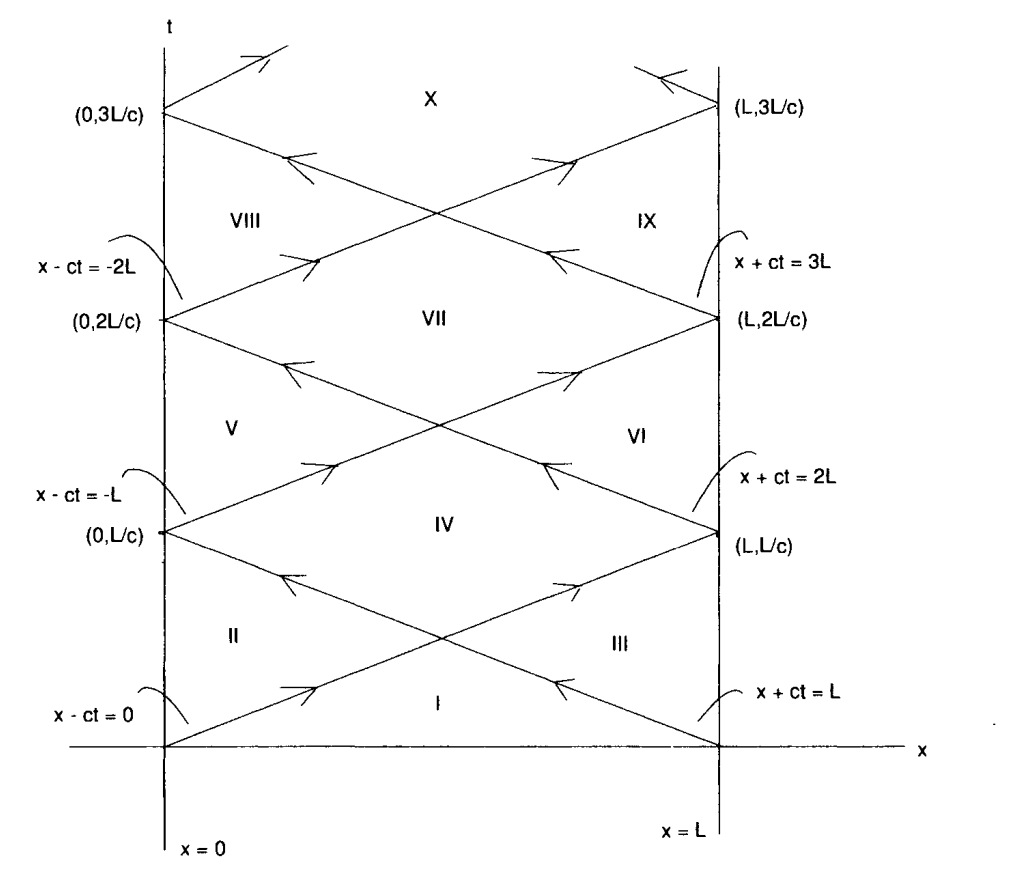
\includegraphics[scale=0.2]{ParticionIntervalo.png}
\end{center}

Sabemos que 
\begin{align*}
    u(x,0) &= \varphi(x)\\
    u(0,t) &= a(t)\\
    u(L,t) &= b(t)
\end{align*}
Y queremos saber $u(x,t)$ para los puntos interiores.

Para esto nos basaremos en el cuadrilátero característico formado por los segmentos de cuatro caracteristicas. $P_{1}$ y $P_{2}$ son vertices opuestos, como lo son $Q_{1}$ y $Q_{2}$. Recurrimos a que si $U$ es una solución, de la ecuación de onda , entonces
\[u(P_{1}) + u(P_{2}) = u(Q_{1}) + u(Q_{2}).\]
Es to es del hecho de que
\[u(x,t) = F(x-ct) + G(x+ct).\]
\begin{center}
    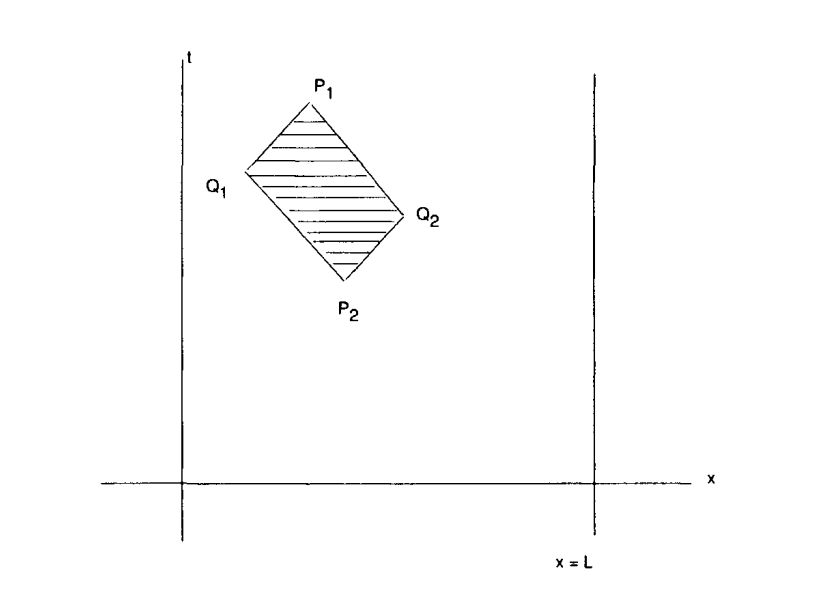
\includegraphics[scale=0.2]{CuadrilateroCaracteristico.png}
\end{center}
Ahora bien, analicemos cada región en la partición del intervalo.

Si $P = (x,t)$ está en la región I, entonces $u(x,t)$ viene dada por la formula de d'Alambert, es decir
\[
u(x,t) = \frac{1}{2}\left( \varphi(x - ct) +  \varphi(x + ct) \right) + \frac{1}{2c} \int_{x-ct}^{x+ct} \psi(s)ds
.\]

Si $P = (x,t)$ está en la región II 
\begin{center}
    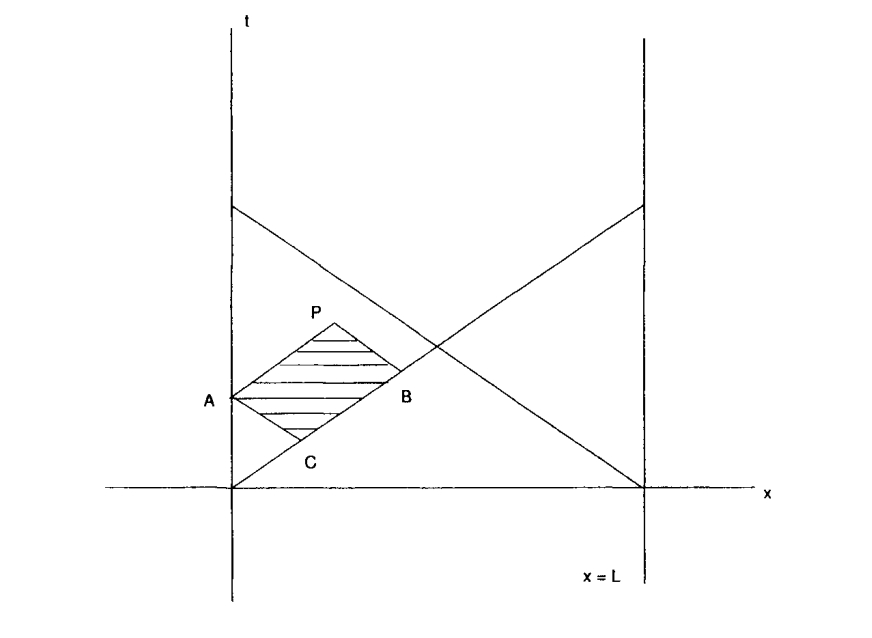
\includegraphics[scale=0.2]{RegionII.png}
\end{center}
Del cuadrilátero característico teniendo un vértice en el eje $x=0$

Obtenemos 
\[
u(P) = u(A) + u(B) - u(C)
.\]
De donde $u(A)$, se conoce de $u(0,t_{A}) = a(t_{A})$. 
También $u(B)$ y $u(C)$, se conocen están en la región I desde la formula de d'Alambert.
\begin{align*}
    u(B) &= \frac{1}{2}\left( \varphi(x_{B} - ct_{B}) +  \varphi(x_{B} + ct_{B}) \right) + \frac{1}{2c} \int_{x_{B}-ct_{B}}^{x_{B}+ct_{B}} \psi(s)ds\\
    u(C) &= \frac{1}{2}\left( \varphi(x_{C} - ct_{C}) +  \varphi(x_{C} + ct_{C}) \right) + \frac{1}{2c} \int_{x_{C}-ct_{C}}^{x_{C}+ct_{C}} \psi(s)ds
\end{align*}

Si $P = (x,t)$ está en la región III 
\begin{center}
    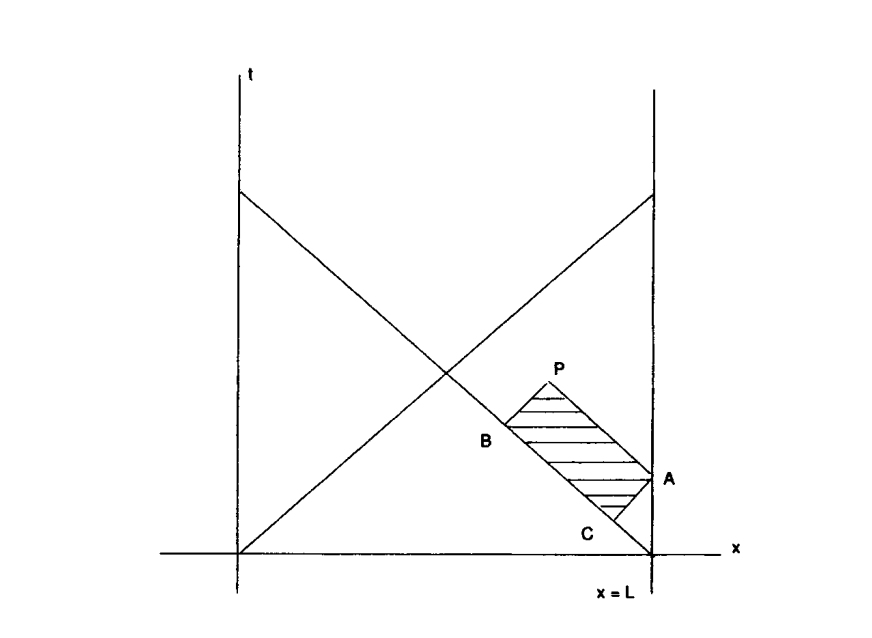
\includegraphics[scale=0.2]{RegionIII.png}
\end{center}
Del cuadrilátero característico teniendo un vértice en el eje $x=L$

Obtenemos 
\[
u(P) = u(A) + u(B) - u(C)
.\]
De donde $u(A)$, se conoce de $u(L,t_{A}) = b(t_{A})$. 
También $u(B)$ y $u(C)$, se conocen están en la región I desde la formula de d'Alambert.
\begin{align*}
    u(B) &= \frac{1}{2}\left( \varphi(x_{B} - ct_{B}) +  \varphi(x_{B} + ct_{B}) \right) + \frac{1}{2c} \int_{x_{B}-ct_{B}}^{x_{B}+ct_{B}} \psi(s)ds\\
    u(C) &= \frac{1}{2}\left( \varphi(x_{C} - ct_{C}) +  \varphi(x_{C} + ct_{C}) \right) + \frac{1}{2c} \int_{x_{C}-ct_{C}}^{x_{C}+ct_{C}} \psi(s)ds
\end{align*}

Si $P = (x,t)$ está en la región IV
\begin{center}
    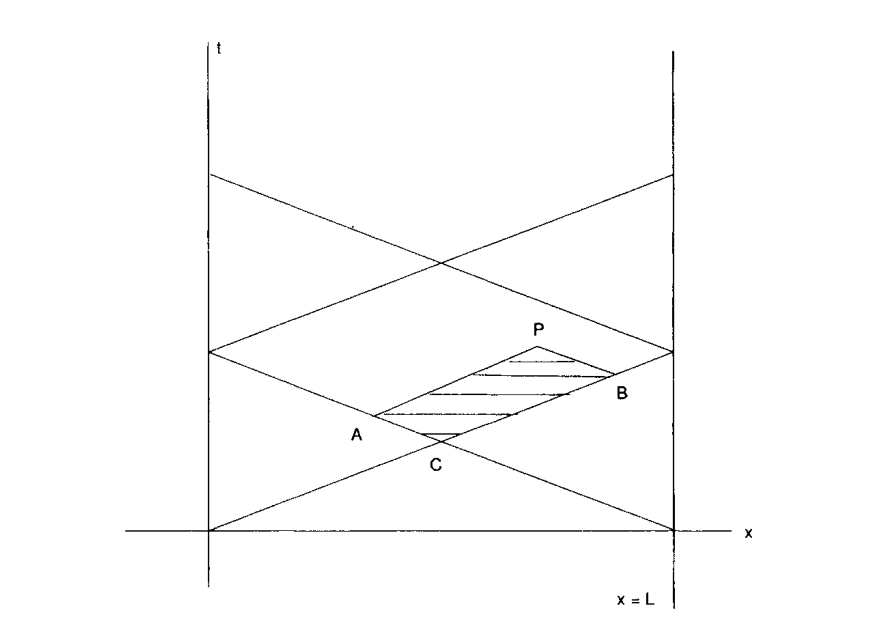
\includegraphics[scale=0.2]{RegionIV.png}
\end{center}
Del cuadrilátero característico teniendo un vértice en el eje $x=L$

Obtenemos 
\[
u(P) = u(A) + u(B) - u(C)
.\]
De donde $u(C)$, se conoce de pues está en la región I. 
También $u(A)$ y $u(B)$, se conocen están en la región II y III.

Y con este mismo proceso se puede seguir para el resto de regiones de manera recursiva se tiene que una región depende de las anteriores, que se tienen definidas.

\section{Solución por series de Fourier al problema sobre un intervalo cerrado}
Analicemos el problema
\setcounter{equation}{0}
\begin{align}
    \frac{\partial^2 u}{\partial t^2} &= c^2 \frac{\partial^2 u}{\partial x^2} \hspace{30mm} 0<x<L, t > 0\\ 
    u(x,0)&= \varphi(x) \hspace{4mm} \frac{\partial u}{\partial t}(x,0) = \psi(x)  \hspace{10mm} 0\leq x\leq L\\
    u(0,t)&= u(L,t) = 0  \hspace{30mm} 0\leq x\leq L
\end{align}

Usaremos un método llamado \emph{separación de variables}, consiste en suponer una solución de la forma $u(x,t) = X(x)T(t)$, el producto de dos funciones de $x$ y de $t$ respectivamente. Al substituir en la ecuación obtenemos
\[
XT'' = c^{2}X''T
.\]
o equivalente
\[
\frac{T''}{c^{2}T} = \frac{X''}{X}
.\]
En ambos lados tenemos funciones que solo dependen de una variable $t$ en la izquierda y $x$ en la derecha, y cada ecuación se puede resolver por medio de separación de variables porque $x$ y $t$ son variables independientes.
Por lo que podemos resolver

\[
\frac{T''}{c^{2}T} = -\lambda \hspace{16mm} \frac{X''}{X} = - \lambda
.\]
Dado que $u(0,t) = X(0)T(0) = 0$ para todo $t$, podemos inferir que $X(0) = 0$, y similarmente $u(L,t) = X(L)T(L) = 0$ implicaría que $X(L) = 0$. Aunque note que también puede ser que $T(t) = 0$ para $t$ tal que $u(x,t) = 0$. 

El problema para $X$, 
\begin{align}
    X'' + \lambda X = 0 \hspace{8mm} X(0) = X(L) = 0
\end{align}
Buscamos valores de $\lambda$, llamados \emph{valores propios}, para los cuales hay soluciones no triviales para $X$, llamada \emph{función propia}, satisfaciendo la ecuación ordinaria, con los valores de frontera.

Notemos que existen algunas posibilidades para $\lambda$.

Si $\lambda = 0$, entonces $X'' = 0$ y $X(x) = ax+b$ para algunas constantes $a$ y $b$. Pero $X(0) = 0$ implica $b=0$, y $X(L) = 0$ implica que $a = 0$, pero esta es una solución trivial.

Si $\lambda < 0$ supongamos $\lambda = -k^{2}$, con $k > 0$, entonces $X'' -k^{2} X = 0$, luego
\[X(x) = a e^{kx} + be^{-kx}.\]
Ahora bien $X(0) = a+b = 0$, $a = -b$, así
\[X(x) = a \left(e^{kx} - e^{-kx}\right).\]
Si $a \neq 0$, entonces $X(L) = a \left(e^{kL} - e^{-kL}\right) = 0$, por lo que $kL = 0$ pero esto es imposible si $k$ y $L$ son no nulos. Lo que implica que $a = 0$, y tenemos una solución trivial.

Si $\lambda > 0$ supongamos $\lambda = k^{2}$, con $k > 0$, entonces $X'' -k^{2} X = 0$, luego
\[X(x) = acos(kx) + bsen(kx).\]
Ahora bien $X(0) = a = 0$,  así
\[X(x) = bsen(kx).\]
Si $b \neq 0$, entonces $X(L) = bsen(kL) = 0$, por lo que $kL = n\pi$, para $n\in\N$, los negativos no nos sirven porque buscamos un sistema linealmente independientes, y recuerde que $sen(x)$ es una función impar. 
\[kL = n\pi \hspace{8mm} n\in\N.\]
Entonces $k = \frac{n\pi}{L}$, y obtenemos valores propios
\[\lambda_{n} = k^{2} = \frac{n^{2}\pi^{2}}{L^{2}} \hspace{8mm} n\in\N.\]
y su función propia correspondiente
\[X_{n}(x) = sen(\frac{n\pi x}{L}).\]
Multiplicada por cualquier constante no nula.

Ahora que sabemos los valores admitidos para $\lambda$ y su correspondiente solución para $X$, el problema para $T$ es
\[
T'' + \frac{n^{2}\pi^{2}}{L^{2}} T = 0
.\]
Con solución general 
\[T_n(t) = a_{n}cos\left(\frac{n\pi ct}{L}\right) + b_{n}sen\left(\frac{n\pi ct}{L}\right).\]
para $n\in\N$
Para todo $n\in\N$, tenemos una función
\begin{align}
    u_{n}(x,t) &= X_{n}(x)T_n(t)\\
    &=\left(a_{n}cos\left(\frac{n\pi ct}{L}\right) + b_{n}sen\left(\frac{n\pi ct}{L}\right)\right)sen(\frac{n\pi x}{L})
\end{align}
Satisfaciendo la ecuación de onda con la condición de frontera $u(0,t) = u(L,t) = 0$. Los que sigue es encontrar una solución que satisfaga la condición inicial.

Notemos que cada $u_n(x)$ es una solución, y podemos pensar en $u(x,t)$ como una superposición de todas las funciones $u_n$
\begin{align*}
    u(x,t) &= \sum_{n\in\N} u_{n}(x,t)\\
    &= \sum_{n\in\N} \left(a_{n}cos\left(\frac{n\pi ct}{L}\right) + b_{n}sen\left(\frac{n\pi ct}{L}\right)\right)sen(\frac{n\pi x}{L})
\end{align*}
Necesitamos constantes $a_{n}$ y $b_{n}$ tal que $u$ satisfaga la condición inicial. Necesitamos 
\[
u(x,0) = \sum_{n\in\N} a_{n}sen(\frac{n\pi x}{L}) = \varphi(x)
.\]
Por lo tanto
\[
a_{n} = \frac{2}{L}\int_{0}^{L} \varphi(\xi)sen(\frac{n\pi \xi}{L})d\xi
.\]
Y además como
\[
\frac{\partial u}{\partial t}(x,t) = \sum_{n\in\N} \frac{n\pi c}{L}\left(-a_{n}sen\left(\frac{n\pi ct}{L}\right) + b_{n}cos\left(\frac{n\pi ct}{L}\right)\right)sen(\frac{n\pi x}{L})
.\]
entonces
\[
\frac{\partial u}{\partial t}(x,0) = \sum_{n\in\N} \frac{n\pi c}{L}b_{n}sen(\frac{n\pi x}{L})
.\]
Por lo tanto
\[
\frac{n\pi c}{L}b_{n} = \frac{2}{L}\int_{0}^{L} \psi(\xi)sen(\frac{n\pi \xi}{L})d\xi
.\]
o también
\[
b_{n} = \frac{2}{n\pi c}\int_{0}^{L} \psi(\xi)sen(\frac{n\pi \xi}{L})d\xi
.\]

\begin{obs}
Observemos que
    \begin{itemize}
        \item Se puede derivar la serie de Fourier, a partir de la serie de derivadas, por la convergencia uniforme de la serie a partir del criterio de Weierstrass.
        \begin{teo}[Criterio de Weierstrass para la convergencia uniforme de series]
            Si \(\{ g_n(x) \}\) es una sucesión de funciones definidas en un conjunto \( E \) y si existe una sucesión de números no negativos \(\{ M_n \}\) tal que:
                \begin{enumerate}
                    \item \( |g_n(x)| \leq M_n \) para todo \( n \) y para todo \( x \) en \( E \), y
                    \item La serie \( \sum M_n \) es convergente,
                \end{enumerate}
                Entonces, la serie \( \sum g_n(x) \) es uniformemente convergente en \( E \). 
        \end{teo}
        Y además en estas condiciones
                \[ \frac{d}{dx}\left( \sum g_n(t) \right) dt = \sum \frac{d g_n(x)}{dx} \]
                \[ \int_a^b \left( \sum g_n(x) \right) dx = \sum \int_a^b \frac{d g_n(x)}{dx} dx \]
    \end{itemize}
\end{obs}

\section{Comparación de las soluciones de Fourier y d'Alambert}
La solución de Fourier es
\begin{align*}
    u(x,t) &= \sum_{n\in\N} \left(a_{n}cos\left(\frac{n\pi ct}{L}\right) + b_{n}sen\left(\frac{n\pi ct}{L}\right)\right)sen(\frac{n\pi x}{L})
\end{align*}
donde $a_{n}$ y $b_{n}$ son las constantes de Fourier.
\begin{align*}
    a_{n} &= \frac{2}{L}\int_{0}^{L} \varphi(\xi)sen(\frac{n\pi \xi}{L})d\xi\\
    b_{n} &= \frac{2}{n\pi c}\int_{0}^{L} \psi(\xi)sen(\frac{n\pi \xi}{L})d\xi
\end{align*}

para el problema con $x\in[0,L]$, $t\geq 0$, $u(0,t) = u(L,t) = 0$, $u(x,0) = \varphi(x)$, $\frac{\partial u}{\partial t}(x,0) = \psi(x)$. Define una extensión par de esta función a $x\in[-L,L]$, $t\geq 0$, $u(-x,t) = u(x,t)$, $u(x+2L,t) = u(x,t)$, $u(x,0) = \varphi(x)$, $\frac{\partial u}{\partial t}(x,0) = \psi(x)$, y de esta extensión periodica $\varphi_{p}(x)$ de $\varphi(x)$ y $\psi_{p}(x)$ de $\psi(x)$ a la recta real. Ahora podemos escribir la solución de d'Alambert es
\begin{align*}
    u(x,t) &= \frac{1}{2}\left( \varphi(x - ct) +  \varphi(x + ct) \right) + \frac{1}{2c} \int_{x-ct}^{x+ct} \psi(s)ds    
\end{align*}
para el problema
\begin{align*}
    \frac{\partial^2 u}{\partial t^2} &= c^2 \frac{\partial^2 u}{\partial x^2} \hspace{30mm} -\infty<x<\infty, t > 0\\ 
    u(x,0)&= \varphi_p(x) \hspace{4mm} \frac{\partial u}{\partial t}(x,0) = \psi_p(x)  \hspace{10mm} -\infty<x<\infty\\
    u(0,t)&= u(L,t) = 0  \hspace{30mm} t\geq 0
\end{align*}
cuando $x$ está restricta a $[0,L]$, esta expresión para $u(x,t)$ también es una solución del problema
\begin{align*}
    \frac{\partial^2 u}{\partial t^2} &= c^2 \frac{\partial^2 u}{\partial x^2} \hspace{30mm} 0<x<L, t > 0\\ 
    u(x,0)&= \varphi(x) \hspace{4mm} \frac{\partial u}{\partial t}(x,0) = \psi(x)  \hspace{10mm} 0\leq x\leq L\\
    u(0,t)&= u(L,t) = 0  \hspace{30mm} 0\leq x\leq L
\end{align*}

\begin{obs}
    Antes vimos que la solución al problema de onda es única, pero en este caso tenemos dos soluciones, la solución de Fourier y la solución de d'Alambert. Por lo tanto tienen que ser iguales.
\end{obs}

\section{Problema no homogéneo sobre un intervalo cerrado}
Analicemos el problema
\setcounter{equation}{0}
\begin{align}
    \frac{\partial^2 u}{\partial t^2} &= c^2 \frac{\partial^2 u}{\partial x^2} + F(x,t) \hspace{30mm} 0<x<L, t > 0\\ 
    u(x,0)&= \varphi(x) \hspace{4mm} \frac{\partial u}{\partial t}(x,0) = \psi(x)  \hspace{10mm} 0\leq x\leq L\\
    u(0,t)&= u(L,t) = 0  \hspace{30mm} 0\leq x\leq L
\end{align}
Este problema se puede abordar por separación de variables. Supongamos que $u(x,t) = X(x)T(t)$, entonces

\[
XT'' = c^{2}X''T + F(x,t)
.\]

supongamos que $u(x,t) = U(x,t) + f(x)$, entonces reemplazando en (1) tenemos
\[
    \frac{\partial^2 U}{\partial t^2} = c^2 \left(\frac{\partial^2 U}{\partial x^2} + \frac{\partial^2 f}{\partial t^2}\right) + F(x,t)
\]
la idea es tomar $f$ tal que:
\[
    \frac{\partial^2 f}{\partial x^2} = -\frac{F(x,t)}{c^2}
.\]
Ahora notemos que 
\[U(0,t) = u(0,t) - f(0) = -f(0)\]
y
\[U(L,t) = u(L,t) - f(L) = -f(L)\]

para $t\geq 0$, por lo que podemos resolver el problema para $U$ con condiciones de frontera homogéneas, y luego sumarle $f(x)$ para obtener la solución para $u$.

Por lo tanto, tomemos $f$ tal que 
\[\frac{\partial^2 f}{\partial x^2} = -\frac{F(x,t)}{c^2} \hspace{8mm} f(0) = f(L) = 0\]

Finalmente, note que para hallar a $U(x,t)$ resolvemos el problema
\setcounter{equation}{0}
\begin{align}
    \frac{\partial^2 U}{\partial t^2} &= c^2 \frac{\partial^2 U}{\partial x^2} \hspace{30mm} 0<x<L, t > 0\\ 
    U(x,0)&= \varphi(x) - f(x) \hspace{4mm} \frac{\partial U}{\partial t}(x,0) = \psi(x) - \frac{\partial f}{\partial t}(x)  \hspace{10mm} 0\leq x\leq L\\
    U(0,t)&= U(L,t) = 0  \hspace{30mm} 0\leq x\leq L
\end{align}
Que ya sabemos resolver, usemos Fourier
\[
    U(x,t) = \sum_{n\in\N} \left(a_{n}cos\left(\frac{n\pi ct}{L}\right) + b_{n}sen\left(\frac{n\pi ct}{L}\right)\right)sen(\frac{n\pi x}{L})
\]
donde 
\begin{align*}
    a_{n} &= \frac{2}{L}\int_{0}^{L} (\varphi(\xi) - f(\xi))sen(\frac{n\pi \xi}{L})d\xi\\
    b_{n} &= \frac{2}{n\pi c}\int_{0}^{L} (\psi(\xi) - \frac{\partial f}{\partial t}(\xi))sen(\frac{n\pi \xi}{L})d\xi
\end{align*}

Y luego la solución para $u$ es
\[
u(x,t) = U(x,t) + f(x)
.\]

\chapter{Ecuación de calor}
\minitoc
La ecuación de calor describe la distribución de temperatura en un cuerpo, y es de la forma

\begin{equation}
    \frac{\partial u}{\partial t} = a^{2} \frac{\partial^2 u}{\partial x^2}
\end{equation}
donde $u(x,t)$ es la temperatura en el punto $x$ y tiempo $t$, y $a^{2}$ es una constante de proporcionalidad. También describe difusión de párticulas quimicas, y la propagación de ondas en un medio con viscosidad.

\texttt{Condiciones iniciales y de contorno:} Para determinar la solución de la ecuación de calor, se requieren condiciones iniciales y de contorno. Las condiciones iniciales especifican la temperatura en el instante inicial
$$u(x,o) = g(x),$$
y las condiciones de contorno especifican la temperatura en los extremos del intervalo 
$$u(0,t) = h_{1}(t) \hspace{4mm} u(L,t) = h_{2}(t).$$

\section{Transferencia de calor en una barra infinita}
Analicemos el problema
\setcounter{equation}{0}
\begin{align}
    \frac{\partial u}{\partial t} &= a^{2} \frac{\partial^2 u}{\partial x^2} \hspace{30mm} -\infty<x<\infty, t > 0\\ 
    u(x,0)&= g(x) \hspace{33mm} -\infty<x<\infty
\end{align}
Aplicamos el metodo de separación de variables, supongamos que $u(x,t) = X(x)T(t)$, entonces
\[
XT' = a^{2}X''T
.\]
o equivalentemente
\[
\frac{T'}{a^{2}T} = \frac{X''}{X}
.\]
En ambos lados tenemos funciones que solo dependen de una variable $t$ en la izquierda y $x$ en la derecha, y cada ecuación se puede resolver por medio de separación de variables porque $x$ y $t$ son variables independientes.

Por lo que podemos resolver
\[
\frac{T'}{a^{2}T} = -\lambda \hspace{16mm} \frac{X''}{X} = - \lambda^{2}
.\]
Con $k$ constante, y $X$ y $T$ funciones de $x$ y $t$ respectivamente.
\[
T' + \lambda a^{2}T = 0
\]
Por lo que $T(t) = C e^{-\lambda a^{2}t}$, y $X$ satisface
\[
X'' + k^{2}X = 0
.\]
Con $X(0) = g(x)$, $X$ es una combinación lineal de $cos(kx)$ y $sen(kx)$, es decir
\[
X(x) = a_{1}cos(\lambda x) + a_{2}sen(\lambda x)
.\]
Sustituyendo en la ecuación inicial
\[
u_{\lambda} = e^{-\lambda a^{2}t}(Ca_{1}cos(\lambda x) + Ca_{2}sen(\lambda x))
.\]
Para cada $\lambda > 0$ tenemos una solución, como la ecuación es lineal, la solución general es una combinación lineal de las soluciones para cada $\lambda$, es decir
\[
u(x,t) = \int_{0}^{\infty} e^{-\lambda a^{2}t}(Ca_{1}cos(\lambda x) + Ca_{2}sen(\lambda x))d\lambda
.\]
siempre que la integral y sus derivadas, segunda respecto a $x$ y primera respecto a $t$, existan.

Reemplazamos en la condición inicial, y tenemos
\[
g(x) = \int_{0}^{\infty} Ca_{1}cos(\lambda x) + Ca_{2}sen(\lambda x))d\lambda
.\]
y por la ortogonalidad de las funciones $cos(\lambda x)$ y $sen(\lambda x)$, tenemos que
\[
a_{1} = \frac{2}{\pi}\int_{0}^{\infty} g(x)cos(\lambda x)dx \hspace{8mm} a_{2} = \frac{2}{\pi}\int_{0}^{\infty} g(x)sen(\lambda x)dx
.\]
Por lo que la solución es
\[
u(x,t) = \frac{2}{\pi}\int_{0}^{\infty} e^{-\lambda a^{2}t}\left(\int_{0}^{\infty} g(\xi)cos(\lambda \xi)d\xi cos(\lambda x) + \int_{0}^{\infty} g(\xi)sen(\lambda \xi)d\xi sen(\lambda x)\right)d\lambda
.\]
y de la integral de Fourier sabemos que
\[
\int_{0}^{\infty} g(\xi)cos(\lambda \xi)d\xi = \frac{1}{\pi}\int_{0}^{\infty} \left(\int_{0}^{\infty} g(\xi)cos(\lambda \xi)d\xi\right)cos(\lambda x)d\lambda
.\]
y
\[
\int_{0}^{\infty} g(\xi)sen(\lambda \xi)d\xi = \frac{1}{\pi}\int_{0}^{\infty} \left(\int_{0}^{\infty} g(\xi)sen(\lambda \xi)d\xi\right)sen(\lambda x)d\lambda
.\]
Por lo que la solución es
\[
u(x,t) = \frac{1}{2a\sqrt{\pi t}}\int_{-\infty}^{\infty}g(\xi)e^{-\frac{(x-\xi)^{2}}{4a^{2}t}}d\xi
.\]
Esta formula es valida para $t>0$, y $x$ y $\xi$ son reales. Se denomina la fórmula de Fourier-Poisson para la ecuación de calor. Observemos que la integral está bien definida para cualquier función $g$ que sea continua, o incluso por partes, en $(-\infty,\infty)$.

\begin{defi}[Núcleo del calor]
    El núcleo del calor es la función definida por partes
    \[
    K(x,t) = 
    \begin{cases} 
    (4\pi a^{2}t)^{-\frac{1}{2}}e^{-\frac{x^{2}}{4a^{2}t}} & \text{si } t > 0, \, x \in \R \\
    0 & \text{si } t < 0, \, x \in \R
    \end{cases}
    \]
\end{defi}

\begin{defi}[Convolución]
    Sean $f$ y $g$ funciones continuas por partes en $(-\infty,\infty)$, definimos la convolución de $f$ y $g$ como
    \[
    (f*g)(x) = \int_{-\infty}^{\infty} f(x-y)g(y)dy
    \]
\end{defi}

Con esta definición, la solución de la ecuación de calor se puede escribir como
\[
u(x,t) = (g*K(\cdot,t))(x)
.\]

\begin{teo}
    Si $g$ es continua por partes en $(-\infty,\infty)$, entonces la solución de la ecuación de calor viene dada por
    \begin{align*}
        u(x,t) &= (g*K(\cdot,t))(x)\\
        &= \int_{-\infty}^{\infty} g(\xi)K(x-\xi,t)d\xi\\
        &= \frac{1}{2a\sqrt{\pi t}}\int_{-\infty}^{\infty}g(\xi)e^{-\frac{(x-\xi)^{2}}{4a^{2}t}}d\xi
    \end{align*}
    para $t>0$ y $x\in\R$.
    \begin{proof}
        Basta ver que $u(x,t)$ satisface la ecuación de calor y las condiciones iniciales. Para la ecuación de calor, note que
        \[\frac{\partial u}{\partial t}(x,t) = \frac{\partial}{\partial t} \int_{-\infty}^{\infty} g(\xi)K(x-\xi,t)d\xi = \int_{-\infty}^{\infty} g(\xi)\frac{\partial}{\partial t} K(x-\xi,t)d\xi\]
        \[\frac{\partial^2 u}{\partial x^2}(x,t) = \frac{\partial^2}{\partial x^2} \int_{-\infty}^{\infty} g(\xi)K(x-\xi,t)d\xi = \int_{-\infty}^{\infty} g(\xi)\frac{\partial^2}{\partial x^2} K(x-\xi,t)d\xi\]
        Luego
        \[\frac{\partial u}{\partial t}(x,t) = \int_{-\infty}^{\infty} g(\xi)\frac{\partial}{\partial t} K(x-\xi,t)d\xi = \int_{-\infty}^{\infty} g(\xi)a^{2}\frac{\partial^2}{\partial x^2} K(x-\xi,t)d\xi = a^{2}\frac{\partial^2 u}{\partial x^2}(x,t)\]
        pues
        \[\frac{\partial}{\partial t} K(x-\xi,t) = -\frac{1}{2}(4\pi a^{2}t)^{-\frac{1}{2}}e^{-\frac{(x-\xi)^{2}}{4a^{2}t}}\left(-\frac{(x-\xi)^{2}}{4a^{2}t^{2}}\right) = a^{2}\frac{\partial^2}{\partial x^2} K(x-\xi,t)\]
        Para las condiciones iniciales, note que
        \[u(x,0) = \int_{-\infty}^{\infty} g(\xi)K(x-\xi,0)d\xi = \int_{-\infty}^{\infty} g(\xi)\delta(x-\xi)d\xi = g(x)\]
    \end{proof}
\end{teo}

\begin{obs}
    El meter la derivada en la integral se puede hacer por el teorema de Leibniz, que dice que si $f$ es continua por partes y diferenciable en $(-\infty,\infty)$, entonces
    \[
    \frac{d}{dx} \int_{-\infty}^{\infty} f(x,y)y = \int_{-\infty}^{\infty} \frac{\partial}{\partial x} f(x,y)dy  
    \]    
\end{obs}

\section{Ecuación no homogénea de calor en una barra infinita}
Analicemos el problema
\setcounter{equation}{0}
\begin{align}
    \frac{\partial u}{\partial t} &= a^{2} \frac{\partial^2 u}{\partial x^2} + f(x,t) \hspace{30mm} -\infty<x<\infty, t > 0\\ 
    u(x,0)&= g(x) \hspace{33mm} -\infty<x<\infty
\end{align}
Suponiendo que $f \in C^{1}(\R \times (0,\infty))$, y $g$ es continua y acotada.

La idea es resolver la ecuación de calor homogénea en cada nivel $t = s > 0$, y luego sumar (integrar) todas estas soluciones.
\begin{align}
    \frac{\partial u}{\partial t} &= a^{2} \frac{\partial^2 u}{\partial x^2} \hspace{30mm} -\infty<x<\infty, t > 0\\ 
    u(x,s)&= f(x,s) \hspace{33mm} -\infty<x<\infty
\end{align}

denotamos la solución por
\[
u(x,t;s) = \frac{1}{2a\sqrt{\pi (t-s)}}\int_{-\infty}^{\infty}f(\xi,s)e^{-\frac{(x-\xi)^{2}}{4a^{2}(t-s)}}d\xi
.\]
para $t>s$, usando el Teorema (3.1.3) y el cambio de variable $t \to t-s$. Ahora podemos escribir la expresión para la solución de (3.1, 3.2) como 
\begin{align}
u(x,t) &= \int_{0}^{t} u(x,t;s)ds\\
&= \int_{0}^{t} \int_{-\infty}^{\infty} K(x-\xi,t-s)f(\xi,s)d\xi ds\\
&= \int_{0}^{t} \frac{1}{2a\sqrt{\pi (t-s)}}\int_{-\infty}^{\infty}f(\xi,s)e^{-\frac{(x-\xi)^{2}}{4a^{2}(t-s)}}d\xi ds
\end{align}

\section{Principios de Máximos y minimos}
Usando notación de operador lineal
\[
L u = a^{2} \frac{\partial^2 u}{\partial x^2} - \frac{\partial u}{\partial t}
.\]
\begin{lema}
    Sea $\Omega \subseteq \R^{2}$ un conjunto abierto, y $u \in C^{2}(\Omega)$ tal que $Lu > 0$ en $\Omega$. Entonces $u$ no puede tener un máximo local en $\Omega$.
    \begin{proof}
        Supongamos que $u$ tiene un máximo local en $(x_{0},t_{0}) \in \Omega$. Entonces $\nabla u(x_{0},t_{0}) = 0$, y por el teorema de Taylor
        \[
            \frac{\partial u}{\partial t}(x_{0},t_{0}) = 0
        \]
        \[
            \frac{\partial^2 u}{\partial x^2}(x_{0},t_{0}) \leq 0
        \]
        Por lo que
        \[
            Lu(x_{0},t_{0}) = \frac{\partial u}{\partial t}(x_{0},t_{0}) - a^{2} \frac{\partial^2 u}{\partial x^2}(x_{0},t_{0}) \leq 0
        \]
        Lo que es una contradicción.
    \end{proof}
\end{lema}

\begin{coro}
    Sea $\Omega \subseteq \R^{2}$ un dominio acotado, y $u \in C^{2}(\Omega)\cap C(\overline{\Omega})$ tal que $Lu \geq 0$ en $\Omega$. Entonces $u$ alcanza su máximo en $\partial \Omega$.
    \begin{proof}
        Como $u$ es continua en $\overline{\Omega}$, alcanza su máximo en $\overline{\Omega}$, y por el lema anterior, no puede alcanzar su máximo en $\overline{\Omega} \setminus \partial \Omega$, por lo que alcanza su máximo en $\partial \Omega$.
    \end{proof}
\end{coro}

\begin{coro}
    Sea $\Omega \subseteq \R^{2}$ un conjunto abierto, y $u \in C^{2}(\Omega)$ tal que $Lu < 0$ en $\Omega$. Entonces $u$ no puede tener un mínimo local en $\Omega$.
    \begin{proof}
        Supongamos que $u$ tiene un mínimo local en $(x_{0},t_{0}) \in \Omega$. Entonces $\nabla u(x_{0},t_{0}) = 0$, y por el teorema de Taylor
        \[
            \frac{\partial u}{\partial t}(x_{0},t_{0}) = 0
        \]
        \[
            \frac{\partial^2 u}{\partial x^2}(x_{0},t_{0}) \geq 0
        \]
        Por lo que
        \[
            Lu(x_{0},t_{0}) = \frac{\partial u}{\partial t}(x_{0},t_{0}) - a^{2} \frac{\partial^2 u}{\partial x^2}(x_{0},t_{0}) \geq 0
        \]
    \end{proof}
\end{coro}

\begin{teo}[Principio del máximo para el operador $L$]
    Sean $\Omega = (a,b)\times(0,T)$, 
    \begin{align*}
        \Gamma_{1} &= \{(x,t) \in \Omega : x = a\}\\
        \Gamma_{2} &= \{(x,t) \in \Omega : t = 0\}\\
        \Gamma_{3} &= \{(x,t) \in \Omega : x = b\}\\
        \Gamma_{4} &= \{(x,t) \in \Omega : t = T\}
    \end{align*}
    Supongamos que $u: \overline{\Omega} \to \R$ es de clase $C^{2}$ en $\Omega\cup\Gamma_{4}$, y $C^{1}$ en $\overline{\Omega}$. Si $Lu \geq 0$ en $\Omega$, entonces $u$ alcanza su máximo en $\Gamma_{1}\cup\Gamma_{2}\cup\Gamma_{3}$.
    \begin{proof}
        Sea $m = max\{u(x,t) : (x,t) \in \Gamma_{1}\cup\Gamma_{2}\cup\Gamma_{3}\}$, y sea $M = max\{u(x,t) : (x,t) \in \overline{\Omega}\}$. Supongamos que $M \in \Gamma_{4}$, entonces $M = u(x_{0},T)$ para algún $x_{0} \in (a,b)$. Sea
        \[
        v(x) = \frac{(M-m) (x-x_{0})}{2(b-a)^{2}}    
        \]    
        y sea
        \[
        w(x,t) = u(x,t) - v(x)
        \]
        Por lo que
        \begin{align*}
            L(w(x,t)) &= L(u(x,t) - v(x))\\
            &= Lu(x,t) + Lv(x)\\
            &= Lu(x,t) + a^{2}\frac{(M-m)}{2(b-a)^{2}}\\
            &= a^{2} \frac{\partial^2 u}{\partial x^2} - \frac{\partial u}{\partial t} + a^{2}\frac{(M-m)}{2(b-a)^{2}}
        \end{align*}
        por hipotesis $Lu \geq 0$, y $\frac{(M-m)}{2(b-a)^{2}} > 0$, por lo que $L(w(x,t)) > 0$, y por el lema (3.3.1) $w(x,t)$ tiene máximo local en $\partial \Omega$. Además $max\{v\} < \frac{M-m}{2} < M$.

        sea $(x,t) \in \Gamma_{1}\cup\Gamma_{2}\cup\Gamma_{3}$, entonces $w(x,t) = u(x,t) - v(x) \leq u(x,t) \leq M$ que es el máximo de $w(x,t)$, por lo que $w(x,t) = M$, y por lo tanto $u(x,t) = M$.
        pero $\frac{\partial w}{\partial t} < 0$ los que es una contradicción, pues $w$ sería decreciente respecto a $t$.
    \end{proof}
\end{teo}

\begin{coro}
    Sea $\Omega$, $\Gamma_{1}$, $\Gamma_{2}$, $\Gamma_{3}$ y $\Gamma_{4}$ como en el teorema anterior y $u \in C^{2}(\Omega \cap \Gamma_{4})\cap C(\overline{\Omega})$. Si $Lu \leq 0$ en $\Omega\cup\Gamma_{4}$. Entonces $u$ alcanza su mínimo en $\Gamma_{1}\cup\Gamma_{2}\cup\Gamma_{3}$. En particular, si $Lu = 0$ en $\Omega\cup\Gamma_{4}$, el máximo y el mínimo de $u$ se alcanzan en $\Gamma_{1}\cup\Gamma_{2}\cup\Gamma_{3}$.
    \begin{proof}
        Sea $v = -u$, entonces $Lv \geq 0$ en $\Omega\cup\Gamma_{4}$, por lo que $v$ alcanza su máximo en $\Gamma_{1}\cup\Gamma_{2}\cup\Gamma_{3}$, y por lo tanto $u$ alcanza su mínimo en $\Gamma_{1}\cup\Gamma_{2}\cup\Gamma_{3}$.
    \end{proof}
\end{coro}

\begin{teo}
    Sea $f \in C([a,b])$, $A, B\in C([0,\infty))$ y $g\in C^{1}((a,b)\times(0,\infty))$. Entonces existe a lo sumo una solución para el problema
    \begin{align*}
        \frac{\partial u}{\partial t} &= a^{2} \frac{\partial^2 u}{\partial x^2} + f(x) \hspace{30mm} a<x<b, t > 0\\ 
        u(x,0)&= A(x) \hspace{33mm} a<x<b\\
        u(a,t)&= B(t) \hspace{33mm} t>0
    \end{align*}
    con $u \in C^{2}((a,b)\times(0,\infty))\cap C([a,b]\times[0,\infty])$ acotada.
    \begin{proof}
        Supongamos que $u_{1}$ y $u_{2}$ son soluciones del problema, y sea $w = u_{1} - u_{2}$. Entonces $w$ satisface
        \begin{align*}
            \frac{\partial w}{\partial t} &= a^{2} \frac{\partial^2 w}{\partial x^2} \hspace{30mm} a<x<b, t > 0\\ 
            w(x,0)&= 0 \hspace{33mm} a<x<b\\
            w(a,t)&= 0 \hspace{33mm} t>0
        \end{align*}
        Por el teorema (3.3.3) $w$ alcanza su máximo en $\partial \Omega$, pero $w(a,t) = 0$ para $t>0$, por lo que $w$ alcanza su máximo en $\Gamma_{1}\cup\Gamma_{2}\cup\Gamma_{3}$, y por lo tanto $w = 0$ en $\Gamma_{1}\cup\Gamma_{2}\cup\Gamma_{3}$, luego $w = 0$ en $\Omega$, por lo que $u_{1} = u_{2}$.
    \end{proof}
\end{teo}

\begin{teo}
    sea $g \in C^{2}(\R\times(0,\infty))$, $f \in C(\R)$ acotada. Entonces existe a lo máximo una solución del problema
    \begin{align*}
        \frac{\partial u}{\partial t} &= a^{2} \frac{\partial^2 u}{\partial x^2} + f(x) \hspace{30mm} -\infty<x<\infty, t > 0\\ 
        u(x,0)&= g(x) \hspace{33mm} -\infty<x<\infty
    \end{align*}
    con $u \in C^{2}((a,b)\times(0,\infty))\cap C([a,b]\times[0,\infty])$ acotada.
    \begin{proof}
        Supongamos que $u_{1}$ y $u_{2}$ son soluciones del problema, y sea $w = u_{1} - u_{2}$. Entonces $w$ satisface
        \begin{align*}
            \frac{\partial w}{\partial t} &= a^{2} \frac{\partial^2 w}{\partial x^2} \hspace{30mm} -\infty<x<\infty, t > 0\\ 
            w(x,0)&= 0 \hspace{33mm} -\infty<x<\infty
        \end{align*}
        existe $M > 0$ tal que $|w(x,t)| \leq M$ para todo $(x,t) \in \overline{\Omega}$. Sea $\alpha > 04 $ tomemos
        \[
            v: \R\times(0,\infty) \to \R \hspace{10mm} v(x,t) = w(x,t) - \frac{M}{a^{2}}x^{2} -2\frac{Ma^{2}}{\alpha^{2}}t
        \]
        Por lo tanto 
        \[
            Lv = 2\frac{Ma^{2}}{\alpha^{2}} - \frac{M}{a^{2}}2 = 0
        \]
        también tenemos que $w(x,t) \leq \frac{M}{a^{2}}x^{2} +2\frac{Ma^{2}}{\alpha^{2}}t$, si $|x| \leq a$, $w \leq 0$ si $a\to\infty$. Por lo que $w = 0$ en $\Omega$, y por lo tanto $u_{1} = u_{2}$.
    \end{proof}
\end{teo}

\section{Ecuación de calor en un intervalo finito}
Analicemos el problema
\setcounter{equation}{0}
\begin{align}
    \frac{\partial u}{\partial t} &= a^{2} \frac{\partial^2 u}{\partial x^2} \hspace{30mm} 0<x<L, t > 0\\ 
    u(x,0)&= g(x) \hspace{33mm} 0<x<L
\end{align}
bajo diferentes condiciones de contorno. Primero consideremos el caso en que $u(0,t) = u(L,t) = 0$ para $t>0$. En este caso, la solución se puede escribir como

Por separación de variables, supongamos que $u(x,t) = X(x)T(t)$, entonces
\[
XT' = a^{2}X''T
.\]
entonces tenemos
\[
\frac{T'}{a^{2}T} = \frac{X''}{X} = -\lambda^{2}
.\]
se toma $\lambda \neq 0$, pues si fuera nulo tenemos soluciones triviales.

Entonces tenemos
\[
T' + \lambda^{2}a^{2}T = 0
\]
\[
X'' + \lambda^{2}X = 0
\]
$X$ y $T$ funciones de $x$ y $t$ respectivamente. Entonces
\[
T(t) = C e^{-\lambda^{2}a^{2}t}
\]
\[
X(x) = a_{1}cos(\lambda x) + a_{2}sen(\lambda x)
\]
Pero $X$ necesita satisfacer la condición de frontera $X(0) = X(L) = 0$, por lo que $a_{1} = 0$, y $X(x) = a_{2}sen(\lambda x)$, y por lo tanto
\[
    \lambda_{n} = \frac{n\pi}{L} \hspace{10mm} n = 1,2,3,\dots
.\]
Es decir 
\[
    X_{n}(x) = sen(\frac{n\pi x}{L})
.\]
para $n = 1,2,3,\dots$. En consectuencia
\[
    T_{n}(t) = C_{n}e^{-\frac{n^{2}\pi^{2}a^{2}t}{L^{2}}}
.\]
Para alguna constante $C_{n}$. Por lo que la solución general es
\[
    u(x,t) = \sum_{n=1}^{\infty} C_{n}e^{-\frac{n^{2}\pi^{2}a^{2}t}{L^{2}}}sen(\frac{n\pi x}{L})
.\]

\begin{obs}
    La solución general es una combinación lineal de las soluciones para cada $\lambda_{n}$, es decir
    \[
        u(x,t) = \sum_{n=1}^{\infty} C_{n}e^{-\frac{n^{2}\pi^{2}a^{2}t}{L^{2}}}sen(\frac{n\pi x}{L})
    .\]
    donde $C_{n}$ son constantes arbitrarias.
\end{obs}

Determinaremos las constantes $C_{n}$ usando la condición inicial. Asumimos que $g$ es continua en $[0,L]$, y que $g(0) = g(L) = 0$. Entonces, tiene expansión como serie de Fourier
\[
    g(x) = \sum_{n=1}^{\infty} g_{n}sen(\frac{n\pi x}{L})
.\]
con
\[
    g_{n} = \frac{2}{L}\int_{0}^{L} g(x)sen(\frac{n\pi x}{L})dx
.\]
para $n = 1,2,3,\dots$. Por lo que tenemos 
\[
    u(x,0) = \sum_{n=1}^{\infty} C_{n}sen(\frac{n\pi x}{L}) = g(x)
.\]
lo que implica que $C_{n} = g_{n}$, y por lo tanto $u$ viene dada por
\[
    u(x,t) = \sum_{n=1}^{\infty} g_{n}e^{-\frac{n^{2}\pi^{2}a^{2}t}{L^{2}}}sen(\frac{n\pi x}{L})
.\]

Veamos que la ecuación efectivamente es solución.
\[
    \frac{\partial u}{\partial t} = \sum_{n=1}^{\infty} -\frac{n^{2}\pi^{2}a^{2}}{L^{2}}g_{n}e^{-\frac{n^{2}\pi^{2}a^{2}t}{L^{2}}}sen(\frac{n\pi x}{L})
.\]
\[
    \frac{\partial^2 u}{\partial x^2} = \sum_{n=1}^{\infty} -\frac{n^{2}\pi^{2}}{L^{2}}g_{n}e^{-\frac{n^{2}\pi^{2}a^{2}t}{L^{2}}}sen(\frac{n\pi x}{L})
.\]
por lo tanto
\[
    \frac{\partial u}{\partial t} = a^{2} \frac{\partial^2 u}{\partial x^2} = \sum_{n=1}^{\infty} \frac{n^{2}\pi^{2}a^{2}}{L^{2}}g_{n}e^{-\frac{n^{2}\pi^{2}a^{2}t}{L^{2}}}sen(\frac{n\pi x}{L})
.\]
\begin{obs}
Se mete la derivada en la integral por el teorema de Weierstrass, que dice que si una serie funcional es acotada término a término por una serie convergente, entonces la serie funcional converge uniformemente. Y si esta converge uniformemente, entonces se puede derivar término a término.
\end{obs}

\section{Condiciones de contorno distintas de cero}
Ahora analicemos el problema
\setcounter{equation}{0}
\begin{align}
    \frac{\partial u}{\partial t} &= a^{2} \frac{\partial^2 u}{\partial x^2} \hspace{30mm} 0<x<L, t > 0\\ 
    u(x,0)&= g(x) \hspace{33mm} 0<x<L\\
    u(0,t)&= u_{1} \hspace{33mm} t>0\\
    u(L,t)&= u_{2} \hspace{33mm} t>0
\end{align}
donde $u_{1}$ y $u_{2}$ son constantes.

Sea $u(x,t) = w(x) + v(x,t)$, donde
\[
    w(x) = \frac{u_{2}-u_{1}}{L}x + u_{1}
.\]
Entonces, si $v(x,t)$ satisface el problema con condiciones de frontera homogéneas
\[
    v(x,t) = \sum_{n=1}^{\infty} g_{n}e^{-\frac{n^{2}\pi^{2}a^{2}t}{L^{2}}}sen(\frac{n\pi x}{L})
\]
entonces $u(x,t) = w(x) + v(x,t)$ satisface el problema original. pues
\[
    u(0,t) = w(0) + v(0,t) = u_{1} + 0 = u_{1}
.\]
\[
    u(L,t) = w(L) + v(L,t) = u_{2} + 0 = u_{2}
.\]
y 
\[
    \frac{\partial u}{\partial t} = \frac{\partial v}{\partial t} = a^{2} \frac{\partial^2 v}{\partial x^2} = a^{2} \frac{\partial^2 u}{\partial x^2}
\]

Ahora bien si $u_{1}, u_{2}$ no son constantes, sino funciones de $t$,
analicemos el problema
\setcounter{equation}{0}
\begin{align}
    \frac{\partial u}{\partial t} &= a^{2} \frac{\partial^2 u}{\partial x^2} \hspace{30mm} 0<x<L, t > 0\\ 
    u(x,0)&= g(x) \hspace{33mm} 0<x<L\\
    u(0,t)&= u_{1}(t) \hspace{33mm} t>0\\
    u(L,t)&= u_{2}(t) \hspace{33mm} t>0
\end{align}

Tenemos la solución general, por separación de variables es de la forma
\[
    u(x,t) = \sum_{n=1}^{\infty} e^{-\frac{n^{2}\pi^{2}a^{2}t}{L^{2}}}\left(a_n sen(\frac{n\pi x}{L}) + bn cos(\frac{n\pi x}{L})\right)
.\]
como $u(x,0) = g(x)$, entonces
\[
    g(x) = \sum_{n=1}^{\infty} a_n sen(\frac{n\pi x}{L})
.\]
por lo que
\[
    a_n = g_{n} =\frac{2}{L}\int_{0}^{L} g(x) sen(\frac{n\pi x}{L})dx
.\]
por otra parte
\[
    u_{1}(t) = \sum_{n=1}^{\infty} b_n e^{-\frac{n^{2}\pi^{2}a^{2}t}{L^{2}}}\
.\]
Y
\[
    u_{2}(t) = \sum_{n=1}^{\infty} (-1)^{n} b_n e^{-\frac{n^{2}\pi^{2}a^{2}t}{L^{2}}}\
.\]
de donde suponemos que $u_{1}(t)$ y $u_{2}(t)$ se pueden escribir como series de esta forma, y por lo tanto tenemos la solución
\[
    u(x,t) = \sum_{n=1}^{\infty} e^{-\frac{n^{2}\pi^{2}a^{2}t}{L^{2}}}\left(g_n sen(\frac{n\pi x}{L}) + b_n cos(\frac{n\pi x}{L})\right)
.\]

\section{Intercambio de calor en los extremos de una barra}
Ahora discutiremos la situación de condiciones de contorno mixtas y reemplazamos las condiciones por
\setcounter{equation}{0}
\begin{align}
    \frac{\partial u}{\partial t} &= a^{2} \frac{\partial^2 u}{\partial x^2} \hspace{30mm} 0<x<L, t > 0\\ 
    u(x,0)&= g(x) \hspace{33mm} 0<x<L\\
    \frac{\partial u}{\partial x}(0,t) - \alpha u(0,t) &= 0 \hspace{33mm} t>0\\
    \frac{\partial u}{\partial x}(L,t) + \alpha u(L,t) &= 0 \hspace{33mm} t>0
\end{align}
para algun $\alpha > 0$. Estas condiciones de frontera se conocen como condiciones de frontera de Robin y representan un intercambio de calor en los extremos de la barra. Cuando $\alpha = 0$ se obtienen condiciones de frontera de Neumann.

Buscamos soluciones de la forma $u(x,t) = X(x)T(t)$, entonces
\[
    XT' = a^{2}X''T
.\]
por lo que
\[
    \frac{T'}{a^{2}T} = \frac{X''}{X} = -\lambda^{2}
.\]
se toma $\lambda \neq 0$, pues si fuera nulo tenemos soluciones triviales. Y las condiciones de contorno
\[
    X'(0) - \alpha X(0) = 0
.\]
\[
    X'(L) + \alpha X(L) = 0
.\]
La solución entonces viene dada por
\[
    X(x) = C_{1}cos(\lambda x) + C_{2}sen(\lambda x)
.\]
con $C_{1}$ y $C_{2}$ satisfaciendo
\[
    \alpha C_{1} - \lambda C_{2} = 0
.\]
\[
    \left(\alpha cos (\lambda L) - \lambda sen(\lambda L)\right)c_{1} + \left(\alpha sen(\lambda L) + \lambda cos(\lambda L)\right)c_{2} = 0
.\]

Para que existan soluciones no triviales, el determinante de este sistema debe ser cero, es decir
\begin{align*}
    0 &=  \alpha \left(\alpha sen(\lambda L) + \lambda cos(\lambda L)\right) - \lambda \left(\alpha cos (\lambda L) - \lambda sen(\lambda L)\right)\\
    &= \alpha^{2}sen(\lambda L) + \alpha \lambda cos(\lambda L) - \alpha \lambda cos(\lambda L) + \lambda^{2}sen(\lambda L)\\
    &= (\alpha^{2} + \lambda^{2})sen(\lambda L)
\end{align*}
por lo tanto
\[
    \lambda_{n} = \frac{n\pi}{L} \hspace{10mm} n = 1,2,3,\dots
.\]
para $n = 1,2,3,\dots$. Para $h > 0$ y $n = 0,1,2,\dots$ definimos $\mu = \lambda L$ y $b = \alpha L$, entonces la ecuación anterior se reduce a
\[
    2cot(\mu) = \frac{\mu}{b} - \frac{b}{\mu}
.\]
que posee soluciones infinitas $\mu_{n}$, $n = 1,2,3,\dots$. Por lo tanto, $\lambda_{n} = \frac{\mu_{n}}{L}$, $n = 1,2,3,\dots$ y las soluciones correspondientes para $X_{n}$ son
\[
    X_{n}(x) = C_{1}cos(\frac{n\pi x}{L}) + C_{2}sen(\frac{n\pi x}{L})
.\]
Podemos ver que 
\[
    \int_{0}^{L} X_{n}(x)X_{m}(x)dx = 0
.\]
Entonces, tomando
\[
    g(x) = \sum_{n=1}^{\infty} g_{n}X_{n}(x)
.\]
con 
\[
    g_{n} = \int_{0}^{L} g(x)X_{n}(x)dx \frac{1}{\int_{0}^{L} X_{n}(x)X_{n}(x)dx}
.\]
de donde esta serie converge absoluta y uniformemente en $[0,L]$, y por lo tanto, dado
\[
    T_{n}(t) = C_{n}e^{-\frac{n^{2}\pi^{2}a^{2}t}{L^{2}}}
.\]
con $C_{n} = g_{n}$, la solución general es
\[
    u(x,t) = \sum_{n=1}^{\infty} = T_{n}(t)X_{n}(x) = \sum_{n=1}^{\infty} g_{n}e^{-\frac{n^{2}\pi^{2}a^{2}t}{L^{2}}}X_{n}(x)
.\]
y para verificar que es solución, basta con verificar que satisface las condiciones de frontera. Tenemos
\[
    u(0,t) = \sum_{n=1}^{\infty} g_{n}e^{-\frac{n^{2}\pi^{2}a^{2}t}{L^{2}}}X_{n}(0) = \sum_{n=1}^{\infty} g_{n}e^{-\frac{n^{2}\pi^{2}a^{2}t}{L^{2}}}X_{n}(L) = u(L,t)
.\]
y
\[
    \frac{\partial u}{\partial x}(0,t) = \sum_{n=1}^{\infty} g_{n}e^{-\frac{n^{2}\pi^{2}a^{2}t}{L^{2}}}\frac{n\pi}{L}X_{n}(0) = \sum_{n=1}^{\infty} g_{n}e^{-\frac{n^{2}\pi^{2}a^{2}t}{L^{2}}}\frac{n\pi}{L}X_{n}(L) = -\alpha u(0,t)
.\]
y
\[
    \frac{\partial u}{\partial x}(L,t) = \sum_{n=1}^{\infty} g_{n}e^{-\frac{n^{2}\pi^{2}a^{2}t}{L^{2}}}\frac{n\pi}{L}X_{n}(L) = \sum_{n=1}^{\infty} g_{n}e^{-\frac{n^{2}\pi^{2}a^{2}t}{L^{2}}}\frac{n\pi}{L}X_{n}(L) = -\alpha u(L,t)
.\]
Además, satisface la ecuación de calor, pues
\[
    \frac{\partial u}{\partial t} = \sum_{n=1}^{\infty} -\frac{n^{2}\pi^{2}a^{2}}{L^{2}}g_{n}e^{-\frac{n^{2}\pi^{2}a^{2}t}{L^{2}}}X_{n}(x)
.\]
\[
    \frac{\partial^2 u}{\partial x^2} = \sum_{n=1}^{\infty} -\frac{n^{2}\pi^{2}}{L^{2}}g_{n}e^{-\frac{n^{2}\pi^{2}a^{2}t}{L^{2}}}X_{n}(x)
.\]
por lo que
\[
    \frac{\partial u}{\partial t} = a^{2} \frac{\partial^2 u}{\partial x^2} = \sum_{n=1}^{\infty} \frac{n^{2}\pi^{2}a^{2}}{L^{2}}g_{n}e^{-\frac{n^{2}\pi^{2}a^{2}t}{L^{2}}}X_{n}(x)
.\]

\section{La transformada de Fourier}

La transformada de Fourier se usa para resolver ecuaciones diferenciales parciales con condiciones de contorno de tipo Dirichlet, Neumann o Robin. La transformada de Fourier se define como

\begin{defi}[Transformada de Fourier]
    Sea $f: \R \to \R$ una función integrable en $\R$. La transformada de Fourier de $f$ es la función $\hat{f}: \R \to \R$ definida por
    \[
        \hat{f}(\lambda) = \int_{-\infty}^{\infty} f(x)e^{-i\lambda x}dx
    \]
    para todo $\lambda \in \R$.
\end{defi}

\begin{ejemplo}
    \begin{itemize}
        \item Sea $f(x) = e^{-|x|}$, entonces
        \begin{align*}
            \hat{f}(\lambda) &= \int_{-\infty}^{\infty} e^{-|x|}e^{-i\lambda x}dx\\
            &= \int_{-\infty}^{0} e^{x}e^{-i\lambda x}dx + \int_{0}^{\infty} e^{-x}e^{-i\lambda x}dx\\
            &= \int_{-\infty}^{0} e^{x-i\lambda x}dx + \int_{0}^{\infty} e^{-x-i\lambda x}dx\\
            &= \int_{-\infty}^{0} e^{x(1-i\lambda)}dx + \int_{0}^{\infty} e^{-x(1+i\lambda)}dx\\
            &= \left[\frac{e^{x(1-i\lambda)}}{1-i\lambda}\right]_{-\infty}^{0} + \left[\frac{e^{-x(1+i\lambda)}}{-1-i\lambda}\right]_{0}^{\infty}\\
            &= \frac{1}{1-i\lambda} + \frac{1}{1+i\lambda}\\
            &= \frac{2}{1+\lambda^{2}}
        \end{align*}
        \item Sea $f(x) = e^{-\alpha |x|}$, entonces
        \begin{align*}
            \hat{f}(\lambda) &= \int_{-\infty}^{\infty} e^{-\alpha |x|}e^{-i\lambda x}dx\\
            &= \int_{-\infty}^{0} e^{\alpha x}e^{-i\lambda x}dx + \int_{0}^{\infty} e^{-\alpha x}e^{-i\lambda x}dx\\
            &= \int_{-\infty}^{0} e^{x(\alpha-i\lambda)}dx + \int_{0}^{\infty} e^{-x(\alpha+i\lambda)}dx\\
            &= \left[\frac{e^{x(\alpha-i\lambda)}}{\alpha-i\lambda}\right]_{-\infty}^{0} + \left[\frac{e^{-x(\alpha+i\lambda)}}{-\alpha-i\lambda}\right]_{0}^{\infty}\\
            &= \frac{1}{\alpha-i\lambda} + \frac{1}{\alpha+i\lambda}\\  
            &= \frac{2\alpha}{\alpha^{2}+\lambda^{2}}
        \end{align*}
    \end{itemize}
\end{ejemplo}

\begin{obs}
    Tabla útil de transformadas.
\begin{center}
    \begin{tabular}{|c|c|}
        \hline
        \( f(t) \) & \( F(\omega) \) \\
        \hline
        \( \delta(t) \) & \( 1 \) \\
        \hline
        \( u(t) \) & \( \frac{1}{j\omega + \epsilon} \) \\
        \hline
        \( e^{at}u(t) \) & \( \frac{1}{j\omega - a} \) \\
        \hline
        \( \sin(at) \) & \( \frac{a}{a^2 + \omega^2} \) \\
        \hline
        \( \cos(at) \) & \( \frac{j\omega}{a^2 + \omega^2} \) \\
        \hline
        \( e^{jat} \) & \( 2\pi \delta(\omega - a) \) \\
        \hline
    \end{tabular}
\end{center}

Si necesitamos hacer la transformada de Fourier respecto a $t$ de una función en dos variables, entonces se considera la variable $x$ como una constante y se aplica la tabla anterior.
\[
    \hat{u}(x,t) = \int_{-\infty}^{\infty} u(x,t)e^{-i\omega t}dt
\]
\end{obs}

\begin{teo}[Propiedades fundamentales de la transformada de Fourier]
    Las siguientes son propiedades de la transformada de Fourier:
    \begin{enumerate}
        \item (Continuidad) Si $f$ es integrable en $\C$, entonces $\hat{f}$ es continua en $\C$.
        \item (Linealidad) Si $f$ y $g$ son integrables en $\C$ y $a,b \in \C$, entonces
        \[
            \widehat{af + bg} = a\hat{f} + b\hat{g}
        \]
        \item (Desplazamiento Tempora) Si $f$ es integrable en $\C$ y $a \in \C$, entonces
        \[
            \widehat{f(t-a)} = e^{-ia\lambda}\hat{f}(\lambda)
        \]
        \item (Desplazamiento en frecuencia) Si $f$ es integrable en $\C$ y $a \in \C$, entonces
        \[
            \widehat{e^{iat}f(t)} = \hat{f}(\lambda - a)
        \]
        \item (Derivada) Si $f$ es integrable en $\C$ y $f'$ es integrable en $\C$, entonces
        \[
            \widehat{f'}(\lambda) = i\lambda \hat{f}(\lambda)
        \]
        \item (Convolución) Si $f$ y $g$ son integrables en $\C$, entonces
        \[
            \widehat{f*g}(\lambda) = \hat{f}(\lambda)\hat{g}(\lambda)
        \]
    \end{enumerate}
\end{teo}
\begin{obs}
    Si se tiene una ecuación diferencial parcial con condiciones de contorno de tipo Dirichlet, Neumann o Robin, se puede aplicar la transformada de Fourier respecto a la variable espacial, y se obtiene una ecuación diferencial ordinaria con condiciones de contorno de tipo Dirichlet, Neumann o Robin. Luego se resuelve la ecuación diferencial ordinaria y se aplica la transformada inversa de Fourier para obtener la solución de la ecuación diferencial parcial.

    Tenemos el siguiente problema
    \setcounter{equation}{0}
    \begin{align}
        \frac{\partial u}{\partial t} &= a^{2} \frac{\partial^2 u}{\partial x^2} \hspace{30mm} 0<x<L, t > 0\\ 
        u(x,0)&= g(x) \hspace{33mm} 0<x<L\\
        u(0,t)&= u_{1}(t) \hspace{33mm} t>0\\
        u(L,t)&= u_{2}(t) \hspace{33mm} t>0
    \end{align}
    donde $u_{1}$ y $u_{2}$ son constantes. Aplicamos la transformada de Fourier respecto a $x$ a la ecuación (1.1), y obtenemos
    \[
        \frac{\partial \hat{u}}{\partial t} = -a^{2}\lambda^{2}\hat{u}
    \]
    con $\hat{u}(\lambda,t) = \int_{0}^{L} u(x,t)e^{-i\lambda x}dx$. Por lo que
    \[
        \hat{u}(\lambda,t) = C(\lambda)e^{-a^{2}\lambda^{2}t}
    \]
    donde $C(\lambda) = \hat{u}(\lambda,0) = \int_{0}^{L} g(x)e^{-i\lambda x}dx$. Por lo que
    \[
        u(x,t) = \int_{-\infty}^{\infty} C(\lambda)e^{-a^{2}\lambda^{2}t}e^{i\lambda x}d\lambda
    \]
    entonces
    \[
        u(x,t) = \int_{-\infty}^{\infty} \hat{u}(\lambda,0)e^{-a^{2}\lambda^{2}t}e^{i\lambda x}d\lambda
    \]
    y por lo tanto
    \[
        u(x,t) = \int_{-\infty}^{\infty} \left(\int_{0}^{L} g(x)e^{-i\lambda x}dx\right)e^{-a^{2}\lambda^{2}t}e^{i\lambda x}d\lambda
    \]
    Que en nuestra notación, con lo que definimos como el nucleo
    \[
        u(x,t) = \frac{1}{2\pi}\int_{-\infty}^{\infty} \hat{g}(\xi)\hat{K}(\xi,t)e^{i\xi x}d\xi
    .\]
    Y al aplicar la transformada inversa de Fourier, obtenemos
    \[
        u(x,t) = (K * g)(x,t).
    .\]
\end{obs}

\chapter{Problemas de Sturm Liouville}
\minitoc
Los problemas de Sturm Liouville son ecuaciones diferenciales ordinarias de segundo orden de la forma
\[
    Lu(x) = \frac{d}{dx}\left(p(x)\frac{du}{dx}\right) + q(x)u = -\lambda \sigma(x)u \hspace{10mm} a<x<b
\]
Se supone que las funciones $p(x)$, $p'(x)$ $q(x)$ y $\sigma(x)$ son continuas en $(a,b)$, y que $p(x) > 0$, $\sigma(x) > 0$ para $x \in [a,b]$. Si el intervalo es finito y se tienen estos supuestos, se dice que el problema es regular. De lo contrario, se dice que el problema es singular.

Introducimos el siguiente producto interno. Para $u,v \in C([a,b])$ definimos
\[
    \langle u,v \rangle = \int_{a}^{b} u(x)v(x)\sigma(x)dx
\]
Si son funciones complejas, se define como
\[
    \langle u,v \rangle = \int_{a}^{b} u(x)\overline{v(x)}\sigma(x)dx
\]

También necesitamos imponer el conjunto de condiciones de contorno hómogeneas.
\begin{align*}
    \alpha_{1}u(a) + \alpha_{2}u'(a) &= 0, \hspace{10mm} |\alpha_{1}| + |\alpha_{2}| > 0\\
    \beta_{1}u(b) + \beta_{2}u'(b) &= 0, \hspace{10mm} |\beta_{1}| + |\beta_{2}| > 0
\end{align*}
donde $\alpha_{1}, \alpha_{2}, \beta_{1}, \beta_{2}$ son constantes reales.

\begin{teo}
    Cualquier operador lineal de segundo ordén se puede escribir en la forma de Sturm-Liouville.
    \[
        Lu = \frac{d}{dx}\left(p(x)\frac{du}{dx}\right) + h(x)u = -\lambda \sigma(x)u
    \]
    \begin{proof}
        Tomemos un operador lineal de segundo orden
        \[
            Lu = \frac{d^{2}u}{dx^{2}} + p(x)\frac{du}{dx} + q(x)u
        \]
        Multiplicando por una función $\sigma(x)$, tenemos
        \[
            \sigma(x)\frac{d^{2}u}{dx^{2}} + \sigma(x)p(x)\frac{du}{dx} + \sigma(x)q(x)u
        \]
        Para que esté en la forma de Sturm-Liouville, necesitamos que
        \[
            \sigma(x)\frac{d^{2}u}{dx^{2}} + \sigma(x)p(x)\frac{du}{dx} = f(x)\frac{d u^{2}}{dx^{2}} + f'(x)\frac{du}{dx} 
        \]
        es decir que 
        \[
            \sigma(x)p(x) = \frac{d \sigma}{dx}
        \]
        lo que es una ecuación diferencial de primer orden, que se puede resolver para $\sigma(x)$, y por lo tanto
        \[
            \sigma(x) = e^{\int_{0}^{x} p(x)dx}
        \]
        y por lo tanto
        \[
            Lu = \frac{d}{dx}\left(e^{\int_{0}^{x} p(x)dx}\frac{du}{dx}\right) + q(x)u
        \]
    \end{proof}
\end{teo}
    \section{Propiedades de los valores propios de Sturm-Liouville}
    Tenemos que un operador diferencial es una transformación lineal de un espacio de funciones a otro.
    \[
        \begin{split}
            L: C^{2}((a,b)) &\to C((a,b))\\
            u &\mapsto Lu = \frac{d}{dx}\left(p(x)\frac{du}{dx}\right) + q(x)u
        \end{split}
    \]
    Por lo que podemos definir los valores propios y vectores propios de un operador diferencial. Tenemos las siguientes propiedades.
    \begin{enumerate}
        \item Los valores propios $\lambda$ son reales, contables, ordenados y hay uno más pequeño. Por lo tanto, se pueden escribir como $\lambda_{1} < \lambda_{2} < \lambda_{3} < \dots$. Sin embargo, no hay un valor propio más grande.
        \item Para cada valor propio $\lambda_{n}$, hay una función propia $\phi_{n}(x)$, con $n-1$ ceros en $(a,b)$.
        \item Las funciones propias correspondientes a valores propios distintos son ortogonales.
        \[
            \langle \phi_{n}, \phi_{m} \rangle = \int_{a}^{b} \phi_{n}(x)\phi_{m}(x)\sigma(x)dx = 0
        \]
        para $n \neq m$. Por lo que podemos escribir la ortogonalidad de las funciones propias como
        \[
            \langle \phi_{n}, \phi_{m} \rangle = \langle \phi_{n}, \phi_{n} \rangle\delta_{nm} \hspace{10mm} n,m = 1,2,3,\dots
        \]
        \item El conjunto de funciones propias $\{\phi_{n}(x)\}_{n=1}^{\infty}$ es completo en el sentido de que cualquier función $f(x) \in L^{2}((a,b))$ se puede escribir como una serie de Fourier
        \[
            f(x) = \sum_{n=1}^{\infty} c_{n}\phi_{n}(x)
        \]
        donde los coeficientes $c_{n}$ están dados por
        \[
            c_{n} = \frac{\langle f, \phi_{n} \rangle}{\langle \phi_{n}, \phi_{n} \rangle}
        \]
        \item Dada una función propia $\phi_{n}(x)$, entonces
        \[
            L \phi_{n}(x) = \lambda_{n}\sigma(x)\phi_{n}(x)
        \]
        Multiplicando por $\phi_{n}(x)$ y tomando el producto interno, tenemos
        \[
            \langle L \phi_{n}, \phi_{n} \rangle = \lambda_{n}\langle \phi_{n}, \phi_{n} \rangle
        \]
        Es decir
        \[
            \langle L \phi_{n}, \phi_{n} \rangle = \int_{a}^{b} \left(\frac{d}{dx}\left(p(x)\frac{d\phi_{n}}{dx}\right) + q(x)\phi_{n}(x)\right)\phi_{n}(x)\sigma(x)dx = \lambda_{n}\int_{a}^{b} \phi_{n}(x)\phi_{n}(x)\sigma(x)dx
        \]
        Solucionamos
        \[
            \frac{d}{dx}\left(p(x)\frac{d\phi_{n}}{dx}\right)|_{a}^{b} - \int_{a}^{b} p(x)\left(\frac{d\phi_{n}}{dx}\right)^{2}dx + \int_{a}^{b} q(x)\phi_{n}^{2}(x)dx = \lambda_{n}\int_{a}^{b} \phi_{n}^{2}(x)\sigma(x)dx
        \]
        Por lo que
        \[
            \lambda_{n} = \frac{\frac{d}{dx}\left(p(x)\frac{d\phi_{n}}{dx}\right)|_{a}^{b} - \int_{a}^{b} p(x)\left(\frac{d\phi_{n}}{dx}\right)^{2}dx + \int_{a}^{b} q(x)\phi_{n}^{2}(x)dx}{\int_{a}^{b} \phi_{n}^{2}(x)\sigma(x)dx}
        \]
        Es decir
        \[
            \lambda_{n} = \frac{\frac{d}{dx}\left(p(x)\frac{d\phi_{n}}{dx}\right)|_{a}^{b} + \int_{a}^{b} \left(p(x)\left(\frac{d\phi_{n}}{dx}\right)^{2} + q(x)\phi_{n}^{2}(x)\right)dx}{\langle \phi_{n}, \phi_{n} \rangle}
        \]
        Que es llamado el cociente de Rayleigh. Es útil para obtener cotas para los valores propios.
    \end{enumerate}

    Cuando se estudió en álgebra lineal, se vio que para un operador lineal $T: V \to W$ entre dos espacios vectoriales finito-dimensionales, se puede definir el operador adjunto $T^{*}: W \to V$ como el operador que satisface
    \[
        \langle Tv, w \rangle_{W} = \langle v, T^{*}w \rangle_{V}
    \]
    A nivel de $\R^{n}$, se puede escribir la transformación de la forma
    \[
        T(x) = Ax
    \]
    Y la adjinta viene dada por
    \[
        Adj(A)_{ij} = (-1)^{i+j}det(A^{ij})
    \]
    donde $A^{ij}$ es la matriz que se obtiene al eliminar la fila $i$ y la columna $j$ de $A$.

    Pero en el contexto de espacios de Hilbert, la cosa es un poco más complicada.
    \begin{defi}
        El dominio de un operador diferencial $L$ es el conjunto de funciones $u(x) \in L^{2}_{\sigma}[a,b]$ que satisface las condiciones de contorno homogéneas y que $Lu \in L^{2}_{\sigma}[a,b]$. El dominio de $L^{*}$ es el conjunto de funciones $v(x) \in L^{2}_{\sigma}[a,b]$ que satisfacen las condiciones de contorno homogéneas.
    \end{defi}

    \begin{defi}
        Sea $L$ un operador entre dos espacios de Hilbert $H_{1}$ y $H_{2}$. El operador adjunto $L^{*}$ de $L$ es el operador definido por
        \[
            \langle Lu, v \rangle_{2} = \langle u, L^{*}v \rangle_{1}
        \]
        Para todo $v$ en el dominio de $L^{*}$ y para todo $u$ en el dominio de $L$.
    \end{defi}

    \begin{ejemplo}
        Tomemos el siguiente operador
        \[
            L = a_2(x)\frac{d^{2}}{dx^{2}} + a_1(x)\frac{d}{dx} + a_0(x)
        \]
        Para hallar el autoadjunto debemos resolver
        \[
            \langle Lu, v \rangle = \langle u, L^{*}v \rangle
        \]
        Por un lado
        \begin{align*}
            \langle Lu, v \rangle &= \int_{a}^{b} \left(a_2(x)\frac{d^{2}u}{dx^{2}} + a_1(x)\frac{du}{dx} + a_0(x)u\right)v(x)dx
        \end{align*}
        Resolvemos cada término por separado.
        \begin{align*}
            \int_{a}^{b} a_2(x)\frac{d^{2}u}{dx^{2}}v(x)dx &= \left[a_2(x)\frac{du}{dx}v(x)\right]_{a}^{b} - \int_{a}^{b} a_2(x)\frac{du}{dx}\frac{dv}{dx}dx\\
            &= \left[a_2(x)\frac{du}{dx}v(x)\right]_{a}^{b} - \int_{a}^{b} \frac{d}{dx}\left(a_2(x)\frac{du}{dx}\right)v(x)dx\\
            &= \left[a_2(x)\frac{du}{dx}v(x)\right]_{a}^{b} - \left[a_2(x)\frac{du}{dx}\right]_{a}^{b} + \int_{a}^{b} \frac{du}{dx}\left(a_2(x)\frac{dv}{dx}\right)dx\\
            &= \left[a_2(x)\frac{du}{dx}v(x)\right]_{a}^{b} - \left[a_2(x)\frac{du}{dx}\right]_{a}^{b} + \left[a_2(x)\frac{dv}{dx}u(x)\right]_{a}^{b} \\
            &- \int_{a}^{b} u(x)\frac{d}{dx}\left(a_2(x)\frac{dv}{dx}\right)dx\\
        \end{align*}
        y
        \begin{align*}
            \int_{a}^{b} a_1(x)\frac{du}{dx}v(x)dx &= \left[a_1(x)u(x)v(x)\right]_{a}^{b} - \int_{a}^{b} a_1(x)u(x)\frac{dv}{dx}dx
        \end{align*}
        entonces
        \begin{align*}
            \langle u, Lv \rangle &= \int_{a}^{b} \left(a_2(x)\frac{d^{2}u}{dx^{2}} + a_1(x)\frac{du}{dx} + a_0(x)u\right)v(x)dx\\
            &= \left[a_2(x)\frac{du}{dx}v(x)\right]_{a}^{b} - \left[a_2(x)\frac{du}{dx}\right]_{a}^{b} + \left[a_2(x)\frac{dv}{dx}u(x)\right]_{a}^{b} \\
            &- \int_{a}^{b} u(x)\frac{d}{dx}\left(a_2(x)\frac{dv}{dx}\right)dx\\
            &+ \left[a_1(x)u(x)v(x)\right]_{a}^{b} - \int_{a}^{b} a_1(x)u(x)\frac{dv}{dx}dx + \int_{a}^{b} a_0(x)u(x)v(x)dx
        \end{align*}
        Aqui queremos que las condiciones iniciales se acomoden para que los terminos que no se están integrando se anulen. Por lo que necesitamos que
        \[
            \left[a_2(x)\frac{du}{dx}v(x)\right]_{a}^{b} - \left[a_2(x)\frac{du}{dx}\right]_{a}^{b} + \left[a_2(x)\frac{dv}{dx}u(x)\right]_{a}^{b} = 0
        \]
        Y
        \begin{align*}
            \langle u, Lv \rangle &= - \int_{a}^{b} u(x)\frac{d}{dx}\left(a_2(x)\frac{dv}{dx}\right)dx - \int_{a}^{b} a_1(x)u(x)\frac{dv}{dx}dx + \int_{a}^{b} a_0(x)u(x)v(x)dx\\
            &= \int_{a}^{b} \left(-u(x)\frac{d}{dx}\left(a_2(x)\frac{dv}{dx}\right) - a_1(x)u(x)\frac{dv}{dx} + a_0(x)u(x)v(x)\right)dx\\
            &= \int_{a}^{b} \left(-\frac{d}{dx}\left(a_2(x)\frac{dv}{dx}\right) - a_1(x)\frac{dv}{dx} + a_0(x)v(x)\right)u(x)dx\\
            &= \langle L^{*}v, u \rangle
        \end{align*}
        Por lo que
        \[
            L^{*}v = -\frac{d}{dx}\left(a_2(x)\frac{dv}{dx}\right) - a_1(x)\frac{dv}{dx} + a_0(x)v(x)
        \]
    \end{ejemplo}

    Antes de pasar a trabajar sobre las pruebas de que los valores propios de un operador de Sturm-Liouville son reales y las funciones propias correspondientes son ortogonales, primero necesitamos introducir dos identidades importantes.
    \begin{teo}[Identidad de Lagrange]
        \[
            uLv - vLu = \frac{d}{dx}\left(p(x)\left(u\frac{dv}{dx} - v\frac{du}{dx}\right)\right)
        \]
        \begin{proof}
            Empecemos desarrollando la izquierda de la igualdad.
            \begin{align*}
                uLv - vLu &= u\frac{d}{dx}\left(p(x)\frac{dv}{dx}\right) + uq(x)v - v\frac{d}{dx}\left(p(x)\frac{du}{dx}\right) - vq(x)u\\
                &= u p(x)\frac{d^{2}v}{dx^{2}} + u\frac{dp}{dx}\frac{dv}{dx} + uq(x)v - v p(x)\frac{d^{2}u}{dx^{2}} - v\frac{dp}{dx}\frac{du}{dx} - vq(x)u\\
                &= u p(x)\frac{d^{2}v}{dx^{2}} + u\frac{dp}{dx}\frac{dv}{dx} - v p(x)\frac{d^{2}u}{dx^{2}} - v\frac{dp}{dx}\frac{du}{dx}\\
                &= \frac{dp}{dx}\left(u\frac{dv}{dx} - v\frac{du}{dx}\right) + p(x)\left(u\frac{d^{2}v}{dx^{2}} - v\frac{d^{2}u}{dx^{2}}\right)\\
            \end{align*}
            Ahora revisemos la derecha de la igualdad.
            \begin{align*}
                \frac{d}{dx}\left(p(x)\left(u\frac{dv}{dx} - v\frac{du}{dx}\right)\right) &= \frac{dp}{dx}\left(u\frac{dv}{dx} - v\frac{du}{dx}\right) + p(x)\frac{d}{dx}\left(u\frac{dv}{dx} - v\frac{du}{dx}\right)\\
                &= \frac{dp}{dx}\left(u\frac{dv}{dx} - v\frac{du}{dx}\right) + p(x)\left(u\frac{d^{2}v}{dx^{2}} + u\frac{dv}{dx} - v\frac{d^{2}u}{dx^{2}} - v\frac{du}{dx}\right)\\
                &= \frac{dp}{dx}\left(u\frac{dv}{dx} - v\frac{du}{dx}\right) + p(x)\left(u\frac{d^{2}v}{dx^{2}} - v\frac{d^{2}u}{dx^{2}}\right)\\ 
            \end{align*}
        \end{proof}
    \end{teo}
    \begin{teo}[La identidad de Green]
        \[
            \int_{a}^{b} \left(uLv - vLu\right)dx = \left(p(x)\left(u\frac{dv}{dx} - v\frac{du}{dx}\right)\right)|_{a}^{b}
        \]
        \begin{proof}
            \begin{align*}
                \int_{a}^{b} \left(uLv - vLu\right)dx &= \int_{a}^{b} \frac{d}{dx}\left(p(x)\left(u\frac{dv}{dx} - v\frac{du}{dx}\right)\right)dx\\
                &= \left(p(x)\left(u\frac{dv}{dx} - v\frac{du}{dx}\right)\right)|_{a}^{b}
            \end{align*}
        \end{proof}
    \end{teo}

    Ahora estamos listos para probar que los valores propios de un operador de Sturm-Liouville son reales y las funciones propias correspondientes son ortogonales. Esto se puede hacer utilizando la identidad de Green.
    \begin{teo}
        Los valores propios de un operador de Sturm-Liouville son reales.
        \begin{proof}
            Tomemos un valor propio $\lambda$ y una función propia $\phi(x)$ correspondiente. Entonces
            \[
                L\phi = \lambda \sigma(x)\phi \hspace{10mm} L\overline{\phi} = \overline{\lambda} \sigma(x)\overline{\phi}
            \]
            hora multiplicamos la primera ecuación por $\overline{\phi}$ y la segunda por $\phi$ y restamos.
            \[
                \overline{\phi}L\phi - \phi L\overline{\phi} = (\lambda - \overline{\lambda})\sigma(x)\phi\overline{\phi}
            \]
            Integramos ambos lados de la igualdad.
            \[
                \int_{a}^{b} \left(\overline{\phi}L\phi - \phi L\overline{\phi}\right)dx = \int_{a}^{b} (\lambda - \overline{\lambda})\sigma(x)\phi\overline{\phi}dx
            \]
            Por la identidad de Green, tenemos
            \[
                \left(p(x)\left(\overline{\phi}\frac{d\phi}{dx} - \phi\frac{d\overline{\phi}}{dx}\right)\right)|_{a}^{b} = \int_{a}^{b} (\lambda - \overline{\lambda})\sigma(x)\phi\overline{\phi}dx
            \]
            usando las condiciones de contorno homogéneas, tenemos
            \[
                \int_{a}^{b} (\lambda - \overline{\lambda})\sigma(x)\phi\overline{\phi}dx = 0
            \]
            Por lo que
            \[
                \lambda = \overline{\lambda}
            \]
            y por lo tanto $\lambda$ es real.
        \end{proof}
    \end{teo}
    \begin{teo}
        Las funciones propias correspondientes a valores propios distintos son ortogonales.
        \begin{proof}
            Tomemos dos valores propios distintos $\lambda_{n}$ y $\lambda_{m}$, y sus funciones propias correspondientes $\phi_{n}(x)$ y $\phi_{m}(x)$. Entonces
            \[
                L\phi_{n} = \lambda_{n}\sigma(x)\phi_{n} \hspace{10mm} L\phi_{m} = \lambda_{m}\sigma(x)\phi_{m}
            \]
            Restamos la primera ecuación multiplicada por $\phi_{m}$ de la segunda ecuación multiplicada por $\phi_{n}$.
            \[
                \phi_{n}L\phi_{m} - \phi_{m}L\phi_{n} = (\lambda_{m} - \lambda_{n})\sigma(x)\phi_{n}\phi_{m}
            \]
            De manera similar al teorema anterior, integramos ambos lados de la igualdad.
            \[
                \int_{a}^{b} \left(\phi_{n}L\phi_{m} - \phi_{m}L\phi_{n}\right)dx = \int_{a}^{b} (\lambda_{m} - \lambda_{n})\sigma(x)\phi_{n}\phi_{m}dx
            \]
            Por la identidad de Green, tenemos
            \[
                \left(p(x)\left(\phi_{n}\frac{d\phi_{m}}{dx} - \phi_{m}\frac{d\phi_{n}}{dx}\right)\right)|_{a}^{b} = \int_{a}^{b} (\lambda_{m} - \lambda_{n})\sigma(x)\phi_{n}\phi_{m}dx
            \]
            usando las condiciones de contorno homogéneas, tenemos
            \[
                \int_{a}^{b} (\lambda_{m} - \lambda_{n})\sigma(x)\phi_{n}\phi_{m}dx = 0
            \]
            Pero los valores propios son distintos, por lo que
            \[
                \int_{a}^{b} \sigma(x)\phi_{n}\phi_{m}dx = 0
            \]
            y por lo tanto
            \[
                \langle \phi_{n}, \phi_{m} \rangle = 0
            \]
            y por lo tanto las funciones propias correspondientes a valores propios distintos son ortogonales.
        \end{proof}
    \end{teo}

\chapter{Ecuación de Laplace}
\minitoc
    La ecuación de Laplace es una ecuación diferencial parcial de segundo orden que se puede escribir como
    \[
        \frac{\partial^{2}u}{\partial x^{2}} + \frac{\partial^{2}u}{\partial y^{2}} = 0
    \]
    En dos dimensiones, o
    \[
        \frac{\partial^{2}u}{\partial x^{2}} + \frac{\partial^{2}u}{\partial y^{2}} + \frac{\partial^{2}u}{\partial z^{2}} = 0
    \]
    En tres dimensiones. La ecuación de Laplace es una ecuación diferencial parcial lineal homogénea, y se puede escribir como
    \[
        \Delta u = 0
    \]
    donde $\Delta: \R^{n} \to \R$ es el operador de Laplace, que se define como
    \[
        \Delta = \sum_{i=1}^{n} \frac{\partial^{2}}{\partial x_{i}^{2}}
    \]
    Debemos tener en cuenta los tipos de condiciones, como ya se ha trabajado antes
    \begin{itemize}
        \item Condiciones de Dirichlet
        \[
            u|_{\partial \Omega}= f
        \]
        \item Condiciones de Neumann
        \[
            \frac{\partial u}{\partial n} = f(x,y)
        \]
        donde $n$ es el vector normal a la frontera $\partial \Omega$.
        \item Condiciones de Robin
        \[
            \alpha u + \beta \frac{\partial u}{\partial n} = f(x,y)
        \]
    \end{itemize}
    \section{Problema de Dirichlet en un rectángulo}
    El problema que vamos a resolver es el siguiente:
    \setcounter{equation}{0}
    \begin{align}
        \frac{\partial^{2}u}{\partial x^{2}} + \frac{\partial^{2}u}{\partial y^{2}} &= 0 \hspace{10mm} 0<x<a, 0<y<b\\
        u(0,y) &= g_{1}(y) \hspace{10mm} 0<y<b\\
        u(a,y) &= g_{2}(y) \hspace{10mm} 0<y<b\\
        u(x,0) &= g_{3}(x) \hspace{10mm} 0<x<a\\
        u(x,b) &= g_{4}(x) \hspace{10mm} 0<x<a
    \end{align}

    Vamos a comenzar con el caso en que $g_{1}(y) = g_{3}(x) = g_{4}(x) = 0$. Entonces queda
    \begin{align*}
        \frac{\partial^{2}u}{\partial x^{2}} + \frac{\partial^{2}u}{\partial y^{2}} &= 0 \hspace{10mm} 0<x<a, 0<y<b\\
        u(0,y) &= 0 \hspace{10mm} 0<y<b\\
        u(a,y) &= f(y) \hspace{10mm} 0<y<b\\
        u(x,0) &= 0 \hspace{10mm} 0<x<a\\
        u(x,b) &= 0 \hspace{10mm} 0<x<a
    \end{align*}
    donde $f\in C^{2}([0,b])$ satisface $f(0) = f(b) = 0$. Para resolver este problema, vamos a utilizar el método de separación de variables. Suponemos que la solución es de la forma
    \[
        u(x,y) = X(x)Y(y)
    \]
    entonces
    \[
        X''(x)Y(y) + X(x)Y''(y) = 0
    \]
    Dividimos por $X(x)Y(y)$ y obtenemos
    \[
        \frac{X''(x)}{X(x)} + \frac{Y''(y)}{Y(y)} = 0
    \]
    Como la primera parte depende solo de $x$ y la segunda solo de $y$, entonces ambas deben ser constantes. Entonces
    \[
        \frac{X''(x)}{X(x)} = \lambda \hspace{10mm} \frac{Y''(y)}{Y(y)} = -\lambda
    \]
    Entonces tenemos dos ecuaciones diferenciales ordinarias de segundo orden. La primera es
    \[
        X''(x) - \lambda X(x) = 0
    \]
    y la segunda es
    \[
        Y''(y) + \lambda Y(y) = 0
    \]
    La primera ecuación tiene soluciones de la forma
    \[
        X(x) = c_{1}e^{\sqrt{\lambda}x} + c_{2}e^{-\sqrt{\lambda}x}
    \]
    y la segunda tiene soluciones de la forma
    \[
        Y(y) = c_{3}\cos(\sqrt{\lambda}y) + c_{4}\sin(\sqrt{\lambda}y)
    \]
    Al aplicar las condiciones de frontera, tenemos
    \[
        X(x) = e^{\sqrt{\lambda}x} - e^{-\sqrt{\lambda}x}
    \]
    y
    \[
        Y(y) = \sin(\sqrt{\lambda}y)
    \]
    Entonces
    \[
        u(x,y) = \sin(\sqrt{\lambda}y)(e^{\sqrt{\lambda}x} - e^{-\sqrt{\lambda}x})
    \]
    y por lo tanto
    \[
        u(x,y) = \sum_{n=1}^{\infty} c_{n}\sin(\sqrt{\lambda_{n}}y)(e^{\sqrt{\lambda_{n}}x} - e^{-\sqrt{\lambda_{n}}x})
    \]
    donde $\lambda_{n} = n^{2}\pi^{2}/a^{2}$ y
    \[
        c_{n} = \frac{2}{b}\int_{0}^{b} f(t)\sin(\sqrt{\lambda_{n}}t)dt
    \]
    Y asi
    \[
        u(x,y) = \frac{2}{b}\sum_{n=1}^{\infty} \left(\int_{0}^{b} f(t)\sin(\sqrt{\lambda_{n}}t)dt\right)\sin(\sqrt{\lambda_{n}}y)(e^{\sqrt{\lambda_{n}}x} - e^{-\sqrt{\lambda_{n}}x})
    \]
    Tomemos
    \[
        K(x,y,t) = \sum_{n=1}^{\infty} \frac{sinh\left(\frac{n\pi x}{b}\right)}{sinh\left(\frac{n\pi a}{b}\right)}\sin\left(\frac{n\pi y}{b}\right)\sin\left(\frac{n\pi t}{b}\right)
    \]
    Entonces
    \[
        u(x,y) = \frac{2}{b}\int_{0}^{b} f(t)K(x,y,t)dt
    \]
    \begin{defi}
        La función $K(x,y,t)$ es llamada el núcleo de Poisson.
    \end{defi}
    \begin{lema}
        La función $K(x,y,t)$ satisface
        \[
            \frac{\partial^{2}K}{\partial x^{2}} + \frac{\partial^{2}K}{\partial y^{2}} = 0 \hspace{10mm} 0<x<a, 0<y<b
        \]
        \begin{proof}
            Tomemos
            \[
                S_{N}(x,y) = \sum_{n=1}^{N} \frac{sinh\left(\frac{n\pi x}{b}\right)}{sinh\left(\frac{n\pi a}{b}\right)}\sin\left(\frac{n\pi t}{b}\right)\sin\left(\frac{n\pi t}{b}\right)
            \]
            Entonces
            \[
                \frac{\partial^{2}S_{N}}{\partial x^{2}} = \sum_{n=1}^{N} \frac{sinh\left(\frac{n\pi x}{b}\right)}{sinh\left(\frac{n\pi a}{b}\right)}\frac{n^{2}\pi^{2}}{b^{2}}\sin\left(\frac{n\pi y}{b}\right)\sin\left(\frac{n\pi t}{b}\right)
            \]
            y
            \[
                \frac{\partial^{2}S_{N}}{\partial y^{2}} = \sum_{n=1}^{N} -\frac{sinh\left(\frac{n\pi x}{b}\right)}{sinh\left(\frac{n\pi a}{b}\right)}\frac{n^{2}\pi^{2}}{b^{2}}\sin\left(\frac{n\pi y}{b}\right)\sin\left(\frac{n\pi t}{b}\right)
            \]
            entonces
            \begin{align*}
                \frac{\partial^{2}S_{N}}{\partial x^{2}} + \frac{\partial^{2}S_{N}}{\partial y^{2}} &= \sum_{n=1}^{N} \frac{sinh\left(\frac{n\pi x}{b}\right)}{sinh\left(\frac{n\pi a}{b}\right)}\frac{n^{2}\pi^{2}}{b^{2}}\sin\left(\frac{n\pi y}{b}\right)\sin\left(\frac{n\pi t}{b}\right)\\
                &- \sum_{n=1}^{N} \frac{sinh\left(\frac{n\pi x}{b}\right)}{sinh\left(\frac{n\pi a}{b}\right)}\frac{n^{2}\pi^{2}}{b^{2}}\sin\left(\frac{n\pi y}{b}\right)\sin\left(\frac{n\pi t}{b}\right)\\
                &= 0    
            \end{align*}
        \end{proof}
    \end{lema}
    \begin{teo}
        Sea $f\in C([0,b])$ diferenciable en $(0,b)$ a menos de un número finito de puntos con $f'$ continua a tramos en $[0,b]$ y $f(0) = f(b) = 0$. Entonces la serie
        \[
            \sum_{n=1}^{\infty} \frac{sinh\left(\frac{n\pi x}{b}\right)}{sinh\left(\frac{n\pi a}{b}\right)}\sin\left(\frac{n\pi t}{b}\right)\sin\left(\frac{n\pi t}{b}\right)
        \]
        converge uniformemente en $[0,b] \times [0,b]$. Y la función $u(x,y)$ definida por
        \[
            u(x,y) = \frac{2}{b}\int_{0}^{b} f(t)K(x,y,t)dt
        \]
        es solución del problema de Dirichlet
        \begin{align*}
            \frac{\partial^{2}u}{\partial x^{2}} + \frac{\partial^{2}u}{\partial y^{2}} &= 0 \hspace{10mm} 0<x<a, 0<y<b\\
            u(0,y) &= 0 \hspace{10mm} 0<y<b\\
            u(a,y) &= f(y) \hspace{10mm} 0<y<b\\
            u(x,0) &= 0 \hspace{10mm} 0<x<a\\
            u(x,b) &= 0 \hspace{10mm} 0<x<a
        \end{align*}
        \begin{proof}
            Para ver la convergencia uniforme, tomemos
            \[
                S_{N}(x,y) = \sum_{n=1}^{N} \frac{sinh\left(\frac{n\pi x}{b}\right)}{sinh\left(\frac{n\pi a}{b}\right)}\sin\left(\frac{n\pi t}{b}\right)\sin\left(\frac{n\pi t}{b}\right)
            \]
            Entonces
            \[
                |S_{N}(x,y)| \leq \sum_{n=1}^{N} \frac{sinh\left(\frac{n\pi x}{b}\right)}{sinh\left(\frac{n\pi a}{b}\right)}\sin\left(\frac{n\pi t}{b}\right)\sin\left(\frac{n\pi t}{b}\right)
            \]
            Luego
            \[
                |S_{N}(x,y)| \leq \sum_{n=1}^{N} \frac{sinh\left(\frac{n\pi x}{b}\right)}{sinh\left(\frac{n\pi a}{b}\right)}
            \]
            Entonces
            \[
                |S_{N}(x,y)| \leq \sum_{n=1}^{N} \frac{e^{\frac{n\pi x}{b}}}{e^{\frac{n\pi a}{b}}}
            \]
            y por lo tanto
            \[
                |S_{N}(x,y)| \leq \sum_{n=1}^{N} e^{\frac{n\pi (x-a)}{b}}
            \]
            Tomando $s = a -x > 0$, tenemos
            \[
                |S_{N}(x,y)| \leq \sum_{n=1}^{N} e^{-\frac{n\pi s}{b}}
            \]
            De la sabemos que la serie converge uniformemente para $s > 0$, por lo que tenemos la convergencia uniforme para $x \in [0,a]$ y $y \in [0,b]$.
            
            Ahora, para ver que $u(x,y)$ es solución del problema de Dirichlet, primero tenemos que ver que $u(x,y)$ es solución de la ecuación de Laplace. Para esto, tomemos
            \[
                u_{x}(x,y) = \frac{2}{b}\int_{0}^{b} f(t)\frac{\partial K}{\partial x}(x,y,t)dt
            \]
            y
            \[
                u_{xx}(x,y) = \frac{2}{b}\int_{0}^{b} f(t)\frac{\partial^{2} K}{\partial x^{2}}(x,y,t)dt
            \]
            y
            \[
                u_{y}(x,y) = \frac{2}{b}\int_{0}^{b} f(t)\frac{\partial K}{\partial y}(x,y,t)dt
            \]
            y
            \[
                u_{yy}(x,y) = \frac{2}{b}\int_{0}^{b} f(t)\frac{\partial^{2} K}{\partial y^{2}}(x,y,t)dt
            \]
            Entonces
            \[
                u_{xx}(x,y) + u_{yy}(x,y) = \frac{2}{b}\int_{0}^{b} f(t)\left(\frac{\partial^{2} K}{\partial x^{2}}(x,y,t) + \frac{\partial^{2} K}{\partial y^{2}}(x,y,t)\right)dt
            \]
            Pero
            \[
                \frac{\partial^{2} K}{\partial x^{2}}(x,y,t) + \frac{\partial^{2} K}{\partial y^{2}}(x,y,t) = 0
            \]
        \end{proof}
    \end{teo}

    \begin{teo}
        Sea $I \subseteq \R$ un intervalo abierto y $F \in C([a,b]\times I)$ es tal que $\frac{\partial F}{\partial x}$ esxiste y es continua en $[a,b]\times I$. Sea
        \[
            f(y) = \int_{a}^{b} F(x,y)dx \hspace{10mm} y \in I
        \]
        Entonces $f \in C^{1}(I)$ y
        \[
            f'(y) = \int_{a}^{b} \frac{\partial F}{\partial y}(x,y)dx \hspace{10mm} y \in I
        \]
    \end{teo}

    Para resolver el problema de Dirichlet en un rectángulo con condiciones de frontera no homogéneas
    \begin{align*}
        \frac{\partial^{2}u}{\partial x^{2}} + \frac{\partial^{2}u}{\partial y^{2}} &= 0 \hspace{10mm} 0<x<a, 0<y<b\\
        u(x,0) &= f_{1}(x) \hspace{10mm} 0<x<a\\
        u(x,b) &= f_{2}(x) \hspace{10mm} 0<x<a\\
        u(0,y) &= g_{1}(y) \hspace{10mm} 0<y<b\\
        u(a,y) &= g_{2}(y) \hspace{10mm} 0<y<b
    \end{align*}
    Vamos a transformarlo al problema que ya sabemos resolver. Para esto, tomemos
    \[
        v(x,y) = u(x,y) - \frac{b-y}{b}g_{2}(0) - \frac{y}{b}g_{2}(b)
    \]
    Entonces si $u$ es solución del problema anterior, entonces $v$ es solución del problema de Dirichlet
    \begin{align*}
        \frac{\partial^{2}v}{\partial x^{2}} + \frac{\partial^{2}v}{\partial y^{2}} &= 0 \hspace{10mm} 0<x<a, 0<y<b\\
        v(x,0) &= F_{1}(x) - g_{2}(0) \hspace{10mm} 0<x<a\\
        v(x,b) &= F_{2}(x) - g_{2}(b) \hspace{10mm} 0<x<a\\
        v(0,y) &= G_{1}(y) \hspace{10mm} 0<y<b\\
        v(a,y) &= G_{2}(y) \hspace{10mm} 0<y<b
    \end{align*}
    donde
    \[
        F_{1}(x) = f_{1}(x) - f_1(a) \hspace{10mm} F_{2}(x) = f_{2}(x) - f_2(a)
    \]
    y
    \[
        G_{1}(y) = g_{1}(y) - \frac{b-y}{b}g_{2}(0) - \frac{y}{b}g_{2}(b) \hspace{10mm} G_{2}(y) = g_{2}(y) - \frac{b-y}{b}g_{2}(0) - \frac{y}{b}g_{2}(b)
    \]
    Observe que $F_{1}(a) = F_{2}(a) = G_{1}(0) = G_{2}(0) = G_{1}(b) = G_{2}(b) = 0$. Observe que el problema de Dirichlet anterior se puede dividir en dos
    \begin{align*}
        \Delta U = 0 \hspace{10mm} 0<x<a, 0<y<b\\
        U(x,0) = F_{1}(x) \hspace{10mm} 0<x<a\\
        U(x,b) = F_{2}(x) \hspace{10mm} 0<x<a\\
        U(0,y) = G_{1}(y) \hspace{10mm} 0<y<b\\
        U(a,y) = 0 \hspace{10mm} 0<y<b
    \end{align*}
    y
    \begin{align*}
        \Delta V = 0 \hspace{10mm} 0<x<a, 0<y<b\\
        V(x,0) = 0 \hspace{10mm} 0<x<a\\
        V(x,b) = 0 \hspace{10mm} 0<x<a\\
        V(0,y) = 0 \hspace{10mm} 0<y<b\\
        V(a,y) = G_{2}(y) \hspace{10mm} 0<y<b
    \end{align*}
    Entonces $v = U + V$ es solución del problema de Dirichlet para $v$. Sabemos resolver para $U$. Para $V$, podemos transformarlo de nuevo a un problema que sabemos resolver. Para esto, tomemos
    \begin{align*}
        \Delta w_1 = 0 \hspace{10mm} 0<x<a, 0<y<b\\
        w_1(x,0) = F_{1}(x) \hspace{10mm} 0<x<a\\
        w_1(x,b) = 0 \hspace{10mm} 0<x<a\\
        w_1(0,y) = 0 \hspace{10mm} 0<y<b\\
        w_1(a,y) = 0 \hspace{10mm} 0<y<b
    \end{align*}
    y
    \begin{align*}
        \Delta w_2 = 0 \hspace{10mm} 0<x<a, 0<y<b\\
        w_2(x,0) = 0 \hspace{10mm} 0<x<a\\
        w_2(x,b) = F_{2}(x) \hspace{10mm} 0<x<a\\
        w_2(0,y) = 0 \hspace{10mm} 0<y<b\\
        w_2(a,y) = 0 \hspace{10mm} 0<y<b
    \end{align*}
    y por ultimo
    \begin{align*}
        \Delta w_3 = 0 \hspace{10mm} 0<x<a, 0<y<b\\
        w_3(x,0) = 0 \hspace{10mm} 0<x<a\\
        w_3(x,b) = 0 \hspace{10mm} 0<x<a\\
        w_3(0,y) = G_{1}(y) \hspace{10mm} 0<y<b\\
        w_3(a,y) = 0 \hspace{10mm} 0<y<b
    \end{align*}
    Note que si sumamos estas soluciones se tien que cumplen las condiciones de frontera de $V$. Entonces $V = w_1 + w_2 + w_3$. Note que $w_1$ es solución del problema de Dirichlet

    \[
        u(x,y) = w_1(x,y) + w_2(x,y) + w_3(x,y) + V(x,y) + \frac{b-y}{b}g_{2}(0) + \frac{y}{b}g_{2}(b)
    \]

    \section{Problema de Dirichlet en un disco unitario}
    \setcounter{equation}{0}
    El problema que resolveremos es el siguiente:
    \begin{align}
        \frac{\partial^{2}u}{\partial x^{2}} + \frac{\partial^{2}u}{\partial y^{2}} &= 0 \hspace{10mm} x,y\in \Omega\\
        u|_{\partial \Omega} &= f
    \end{align}

    donde $\Omega = \{(x,y) \in \R^{2} : x^{2} + y^{2} < 1\}$ y $f \in C(\partial \Omega)$. Vamos a reescribir el problema en coordenadas polares. Para esto, tomemos
    \[
        x = r\cos(\theta) \hspace{10mm} y = r\sin(\theta)
    \]
    donde $r \in [0,1)$ y $\theta \in [0,2\pi)$. Entonces

    Sea $v(r,\theta) = u(r\cos(\theta), r\sin(\theta))$. Entonces
    \begin{align*}
        \frac{\partial v}{\partial r} &= \frac{\partial u}{\partial x}\frac{\partial x}{\partial r} + \frac{\partial u}{\partial y}\frac{\partial y}{\partial r}\\
        &= \cos(\theta)\frac{\partial u}{\partial x} + \sin(\theta)\frac{\partial u}{\partial y}\\
        &= \cos(\theta)v_{x} + \sin(\theta)v_{y}\\
        \frac{\partial^{2} v}{\partial r^{2}} &= \cos(\theta)\frac{\partial}{\partial r}\left(\cos(\theta)v_{x} + \sin(\theta)v_{y}\right) + \sin(\theta)\frac{\partial}{\partial r}\left(\cos(\theta)v_{x} + \sin(\theta)v_{y}\right)\\
        &= \cos^{2}(\theta)v_{xx} + 2\cos(\theta)\sin(\theta)v_{xy} + \sin^{2}(\theta)v_{yy} + \cos(\theta)v_{x} + \sin(\theta)v_{y}\\
        \frac{\partial v}{\partial \theta} &= \frac{\partial u}{\partial x}\frac{\partial x}{\partial \theta} + \frac{\partial u}{\partial y}\frac{\partial y}{\partial \theta}\\
        &= -r\sin(\theta)\frac{\partial u}{\partial x} + r\cos(\theta)\frac{\partial u}{\partial y}\\
        &= -r\sin(\theta)v_{x} + r\cos(\theta)v_{y}
    \end{align*}
    Por lo tanto tenemos
    \begin{align*}
        \frac{\partial^{2} v}{\partial r^{2}} + \frac{1}{r}\frac{\partial v}{\partial r} + \frac{1}{r^{2}}\frac{\partial^{2} v}{\partial \theta^{2}} &= \cos^{2}(\theta)v_{xx} + 2\cos(\theta)\sin(\theta)v_{xy}\\
        &\hspace{4mm}+ \sin^{2}(\theta)v_{yy} + \cos(\theta)v_{x} + \sin(\theta)v_{y}\\
        &\hspace{4mm}+ \frac{1}{r}\left(-r\sin(\theta)v_{x} + r\cos(\theta)v_{y}\right)\\
        &\hspace{4mm}+ \frac{1}{r^{2}}(-r^{2}\sin^{2}(\theta)v_{xx}\\ 
        &\hspace{4mm}- 2r^{2}\sin(\theta)\cos(\theta)v_{xy} - r^{2}\cos^{2}(\theta)v_{yy})\\
        &= \cos^{2}(\theta)v_{xx} + 2\cos(\theta)\sin(\theta)v_{xy} + \sin^{2}(\theta)v_{yy}\\
        &\hspace{4mm}+ \cos(\theta)v_{x} + \sin(\theta)v_{y}\\
        &\hspace{4mm}- \sin(\theta)v_{x} + \cos(\theta)v_{y} - \sin^{2}(\theta)v_{xx}\\
        &\hspace{4mm}- 2\sin(\theta)\cos(\theta)v_{xy} - \cos^{2}(\theta)v_{yy}\\
        &= v_{xx} + v_{yy}\\
        &= 0
    \end{align*}
    Y sustituir en la condición de frontera
    \[
        g(\theta) = f(cos(\theta), sin(\theta)) = v(1,\theta) = u(1\cos(\theta), 1\sin(\theta))
    \]
    Entonces el problema se puede escribir como
    \begin{align*}
        \frac{\partial^{2}v}{\partial r^{2}} + \frac{1}{r}\frac{\partial v}{\partial r} + \frac{1}{r^{2}}\frac{\partial^{2}v}{\partial \theta^{2}} &= 0 \hspace{10mm} 0<r<1, 0<\theta<2\pi\\
        v(1,\theta) &= g(\theta) \hspace{10mm} 0<\theta<2\pi
    \end{align*}
    Vamos a resolver este problema utilizando el método de separación de variables. Supongamos que la solución es de la forma
    \[
        v(r,\theta) = R(r)\Theta(\theta)
    \]
    Entonces
    \[
        R''(r)\Theta(\theta) + \frac{1}{r}R'(r)\Theta(\theta) + \frac{1}{r^{2}}R(r)\Theta''(\theta) = 0
    \]
    o equivalentemente
    \[
        r^{2}R''(r)\Theta(\theta) + rR'(r)\Theta(\theta) + R(r)\Theta''(\theta) = 0
    \]
    Dividimos por $R(r)\Theta(\theta)$ y obtenemos
    \[
        \frac{r^{2}R''(r) + rR'(r)}{R(r)} = -\frac{\Theta''(\theta)}{\Theta(\theta)} = \lambda
    \]
    Entonces tenemos dos ecuaciones diferenciales ordinarias de segundo orden. La primera es
    \[
        \Theta''(\theta) + \lambda\Theta(\theta) = 0
    \]
    y la segunda es
    \[
        r^{2}R''(r) + rR'(r) - \lambda R(r) = 0
    \]
    Analisemos cada una de estas ecuaciones por separado. La primera ecuación, se debe analizar para cada valor de $\lambda$. Si $\lambda = 0$, entonces la solución es
    \[
        \Theta(\theta) = c_{1} + c_{2}\theta
    \]
    Pero la solución debe ser periódica.

    Si $\lambda < 0$, tome $\lambda = -\mu^{2}$, entonces la ecuación se convierte en
    \[
        \Theta''(\theta) - \mu^{2}\Theta(\theta) = 0
    \]
    y la solución es
    \[
        \Theta(\theta) = c_{1}e^{-\mu\theta} + c_{2}e^{\mu\theta}
    \]
    Esta solución no es periódica, por lo que no nos sirve.

    Si $\lambda > 0$, tome $\lambda = \mu^{2}$, entonces la ecuación se convierte en
    \[
        \Theta''(\theta) + \mu^{2}\Theta(\theta) = 0
    \]
    y la solución es
    \[
        \Theta(\theta) = c_{1}\cos(\mu\theta) + c_{2}\sin(\mu\theta)
    \]
    Esta solución es periódica, por lo que nos sirve. Ahora analicemos la segunda ecuación. Ya sabemos que $\lambda = \mu^{2}$. Entonces la ecuación se convierte en
    \[
        r^{2}R''(r) + rR'(r) - \mu^{2} R(r) = 0
    \]
    este es una ecuación de Euler. La solución es de la forma
    \[
        R(r) = r^{\alpha}
    \]
    Entonces
    \[
        \alpha(\alpha - 1)r^{\alpha - 2} + \alpha r^{\alpha - 1} - \mu^{2}r^{\alpha} = 0
    \]
    Dividimos por $r^{\alpha - 2}$ y obtenemos
    \[
        \alpha(\alpha - 1) + \alpha - \mu^{2} = 0
    \]
    Entonces
    \[
        \alpha^{2} - \mu^{2} = 0
    \]
    y por lo tanto
    \[
        \alpha = \pm \mu
    \]
    Entonces la solución es
    \[
        R(r) = c_{1}r^{\mu} + c_{2}r^{-\mu}
    \]
    Es requisito que la solución sea acotada en $r = 0$, por lo que $c_{2} = 0$. Entonces
    \[
        R(r) = c_{1}r^{\mu}
    \]
    y por lo tanto
    \[
        v(r,\theta) = c_{1}r^{\mu}\cos(\mu\theta) + c_{2}r^{\mu}\sin(\mu\theta)
    \]
    Tenga $\mu = n$ con $n \in \N$. Entonces
    \[
        v_{n}(r,\theta) = c_{1}r^{n}\cos(n\theta) + c_{2}r^{n}\sin(n\theta)
    \]
    Y por lo tanto
    \[
        v(r,\theta) = \frac{A_0}{2} + \sum_{n=1}^{\infty} \left(A_{n}r^{n}\cos(n\theta) + B_{n}r^{n}\sin(n\theta)\right)
    \]
    Que tiene la forma de una serie de Fourier. Entonces reemplazamos en la condición de frontera
    \[
        g(\theta) = v(1,\theta) = \frac{A_0}{2} + \sum_{n=1}^{\infty} r^{n}\left(A_{n}\cos(n\theta) + B_{n}\sin(n\theta)\right)
    \]
    entonces
    \[
        r^{n}A_{n} = \frac{1}{\pi}\int_{0}^{2\pi} g(\theta)\cos(n\theta)d\theta
    \]
    y
    \[
        r^{n}B_{n} = \frac{1}{\pi}\int_{0}^{2\pi} g(\theta)\sin(n\theta)d\theta
    \]
    Entonces
    \[
        v(r,\theta) = \frac{\int_{0}^{2\pi} g(\theta)\cos(\theta)d\theta}{2\pi} + \sum_{n=1}^{\infty} \left(\frac{1}{\pi}\int_{0}^{2\pi} g(\theta)\cos(n\theta)d\theta\cos(n\theta) + \frac{1}{\pi}\int_{0}^{2\pi} g(\theta)\sin(n\theta)d\theta\sin(n\theta)\right)
    \]
    La convergencia es uniforme en $[0,1]\times[0,2\pi]$. pues es acotada con la serie de Fourier de $g(\theta)$.
    Por último tenemos que sustituir de nuevo en $v(r,\theta) = u(r\cos(\theta), r\sin(\theta))$. Haciendo el cambio de variable $r = \sqrt{x^{2} + y^{2}}$ y $\theta = \arctan(y/x)$, tenemos
    \begin{align*}
        u(x,y) =& \frac{\int_{0}^{2\pi} g(\theta)\cos(\theta)d\theta}{2\pi}\\
                & + \sum_{n=1}^{\infty} \left(\frac{1}{\pi}\int_{0}^{2\pi} g(\theta)\cos(n\theta)d\theta\cos(n\arctan(y/x))\right)\\
                & + \sum_{n=1}^{\infty} \left(\frac{1}{\pi}\int_{0}^{2\pi} g(\theta)\sin(n\theta)d\theta\sin(n\arctan(y/x))\right)
    \end{align*}

    \section{Las identidades de Green}
    Sea $\Omega \subseteq \R^{n}$ un abierto. Un campo vectorial en $\Omega$ es una función $F : \Omega \to \R^{n}$. Decimos que $F$ es de clase $C^{n}$ si sus componentes son de clase $C^{n}$.
    \begin{defi}[Gradiente de una función]
        Sea $f : \Omega \to \R$ una función de clase $C^{1}$. Definimos el gradiente de $f$ como el campo vectorial dado por
        \[
            \nabla f = \sum_{i=1}^{n} \frac{\partial f}{\partial x_{i}}\ e_{i}
        \]
        Donde $e_{i}$ es el vector unitario en la dirección $x_{i}$.
    \end{defi}
    \begin{defi}[Divergencia de un campo vectorial]
        Sea $F : \Omega \to \R^{n}$ un campo vectorial de clase $C^{1}$. Definimos la divergencia de $F$ como la función dada por
        \[
            \nabla \cdot F = \sum_{i=1}^{n} \frac{\partial F_{i}}{\partial x_{i}}
        \]
    \end{defi}
    Note que si $F = \nabla f$, entonces $\nabla \cdot F = \nabla \cdot \nabla f = \sum_{i=1}^{n} \frac{\partial^{2} f}{\partial x_{i}^{2}}$. Es decir, la divergencia de un gradiente es la traza de la matriz Hessiana.
    \[
        \Delta f = div(grad (f)) = \nabla \cdot \nabla f = \sum_{i=1}^{n} \frac{\partial^{2} f}{\partial x_{i}^{2}}  
    \]
    Nos quedaremos con el caso $n = 2$. En este caso, si $F = (F_{1}, F_{2})$.
    \begin{teo}[Teorema de Green]
        Sea $\Omega \subseteq \R^{2}$ un dominio acotado, y sea $P, Q: \overline{\Omega} \to \R$ funciones de clase $C^{1}$. Suponga que:
        \begin{enumerate}
            \item $\partial \Omega$ es una curva simple y cerrada y rectificable.
            \item Las derivadas parciales $\frac{\partial P}{\partial y}$ y $\frac{\partial Q}{\partial x}$ son continuas en $\Omega$.
            \item Las integrales
            \[
                \int_{\partial \Omega} \frac{\partial Q}{\partial x} dxdy \hspace{10mm} \int_{\partial \Omega} \frac{\partial P}{\partial y} dxdy
            \]
            existen y son finitas.
        \end{enumerate}
        Entonces
        \[
            \int_{\partial \Omega ^{+}} Pdx + Qdy = \int_{\Omega} \left(\frac{\partial Q}{\partial x} - \frac{\partial P}{\partial y}\right)dxdy
        \]

    \end{teo}
    \begin{teo}[Teorema de la Divergencia]
        Sea $\Omega \subseteq \R^{2}$ un dominio acotado cuya frontera $\partial \Omega$ es una curva simple y cerrada y rectificable. Sea $F : \overline{\Omega} \to \R^{2}$ un campo vectorial de clase $C^{1}$. Sea $F : \overline{\Omega} \to \R^{2}$ un campo vectorial de clase $C^{1}$. Entonces
        \[
            \int_{\partial \Omega ^{+}} F \cdot \overrightarrow{n}ds = \int_{\Omega} \nabla \cdot F dxdy  
        \]
        donde $\overrightarrow{n}$ es el vector normal unitario a $\partial \Omega$.
    \end{teo}
    \begin{teo}
        Sea $\Omega \subseteq \R^{2}$ un dominio donde vale el teorema de la divergencia y sean $u, v \in C^{2}(\overline{\Omega})$. Entonces valen las siguentes identidades:
        \begin{align*}
            \int_{\overline{\Omega}} \left(v \Delta u - \nabla u \cdot \nabla v\right)dxdy &= \int_{\partial \Omega} v \frac{\partial u}{\partial n}ds\\
            \int_{\overline{\Omega}} \left(v \Delta u - u \Delta v\right)dxdy &= \int_{\partial \Omega} \left(v \frac{\partial u}{\partial n} - u \frac{\partial v}{\partial n}\right)ds
        \end{align*}
        donde $\frac{\partial u}{\partial n}$ es la derivada en la dirección de la normal unitaria externa a $\partial \Omega$.
        \begin{proof}
            Demostremos primero la primera identidad.
            \[
                \int_{\overline{\Omega}} \left(v \Delta u - \nabla u \cdot \nabla v\right)dxdy = \int_{\overline{\Omega}} \nabla \cdot (v\nabla u) - \nabla \cdot (u\nabla v)dxdy
            \]
            Tomemos la función auxiliar
            \[
                f = v\nabla u  
            \]
            Entonces tenemos que
            \[
                \nabla \cdot f = \nabla \cdot (v\nabla u) = \nabla v \cdot \nabla u + v \Delta u
            \]
            Entonces
            \[
                \int_{\overline{\Omega}} \left(v \Delta u - \nabla u \cdot \nabla v\right)dxdy = \int_{\overline{\Omega}} \nabla \cdot f dxdy
            \]
            Por el teorema de la divergencia
            \[
                \int_{\overline{\Omega}} \nabla \cdot f dxdy = \int_{\partial \Omega} f \cdot \overrightarrow{n}ds
            \]
            Pero
            \[
                f \cdot \overrightarrow{n} = v \frac{\partial u}{\partial n}
            \]
            Entonces
            \[
                \int_{\partial \Omega} f \cdot \overrightarrow{n}ds = \int_{\partial \Omega} v \frac{\partial u}{\partial n}ds
            \]
            Por lo tanto
            \[
                \int_{\overline{\Omega}} \left(v \Delta u - \nabla u \cdot \nabla v\right)dxdy = \int_{\partial \Omega} v \frac{\partial u}{\partial n}ds
            \]
            Ahora demostremos la segunda identidad.
            \[
                \int_{\overline{\Omega}} \left(v \Delta u - u \Delta v\right)dxdy = \int_{\partial \Omega} \left(v \frac{\partial u}{\partial n} - u \frac{\partial v}{\partial n}\right)ds
            \]
            Apliquemos la identidad anterior
            \[
                \int_{\overline{\Omega}} \left(v \Delta u - u \Delta v\right)dxdy - \int_{\overline{\Omega}} \left(v \Delta u - \nabla u \cdot \nabla v\right)dxdy
            \]
            De donde
            \[
                \int_{\overline{\Omega}} \left(v \Delta u - u \Delta v\right)dxdy - \int_{\overline{\Omega}} \left(v \Delta u - \nabla u \cdot \nabla v\right)dxdy = \int_{\partial \Omega} \left(v \frac{\partial u}{\partial n} - u \frac{\partial v}{\partial n}\right)ds
            \]
            Se tiene la identidad.
        \end{proof}
    \end{teo}

    \begin{coro}
        Sea $\Omega \subseteq \R^{2}$ un dominio donde vale el teorema de la divergencia y sean $u \in C^{2}(\overline{\Omega})$ tal que $\Delta u = 0$ en $\Omega$. Entonces valen las siguentes identidades:
        \begin{align*}
            \int_{\overline{\Omega}} |\nabla u|^{2}dxdy &= \int_{\partial \Omega} u \frac{\partial u}{\partial n}ds\\
            \int_{\overline{\Omega}} \frac{\partial u}{\partial n}dxdy &= 0
        \end{align*}
        \begin{proof}
            La primera identidad se obtiene de la primera identidad del teorema anterior tomando $v = u$. pues
            \begin{align*}
                \int_{\overline{\Omega}} \left(u \Delta u - \nabla u \cdot \nabla u\right)dxdy &= \int_{\partial \Omega} u \frac{\partial u}{\partial n}ds\\
                \int_{\overline{\Omega}} \left(u \Delta u - |\nabla u|^{2}\right)dxdy &= \int_{\partial \Omega} u \frac{\partial u}{\partial n}ds\\
                \int_{\overline{\Omega}} |\nabla u|^{2}dxdy &= \int_{\partial \Omega} u \frac{\partial u}{\partial n}ds
            \end{align*}

            Para la sefunda identidad, tomemos $v = 1$ en la segunda identidad del teorema anterior. Entonces
            \begin{align*}
                \int_{\overline{\Omega}} \left(1 \Delta u - u \Delta 1\right)dxdy &= \int_{\partial \Omega} \left(1 \frac{\partial u}{\partial n} - u \frac{\partial 1}{\partial n}\right)ds\\
                \int_{\overline{\Omega}} \left(1 \Delta u - 0\right)dxdy &= \int_{\partial \Omega} \left(1 \frac{\partial u}{\partial n} - 0\right)ds\\
                \int_{\overline{\Omega}} \Delta u dxdy &= \int_{\partial \Omega} \frac{\partial u}{\partial n}ds\\
                \int_{\overline{\Omega}} 0 dxdy &= \int_{\partial \Omega} \frac{\partial u}{\partial n}ds\\
                0 &= \int_{\partial \Omega} \frac{\partial u}{\partial n}ds
            \end{align*}
        \end{proof}        
    \end{coro}
    \begin{coro}
        Sea $\Omega \subseteq \R^{2}$ un dominio donde vale el teorema de la divergencia, $f\in C(\partial \Omega)$ y $u \in C^{2}(\overline{\Omega})$ tal que $\Delta u = 0$ en $\Omega$. Entonces el problema
        \begin{align*}
            \Delta u &= 0 \hspace{10mm} \text{en } \Omega\\
            u &= f \hspace{10mm} \text{en } \partial \Omega
        \end{align*}
        teien a lo más una solución.
        \begin{proof}
            Tome dos soluciones $u_{1}$ y $u_{2}$. Entonces $u = u_{1} - u_{2}$ es solución del problema
            \begin{align*}
                \Delta u &= 0 \hspace{10mm} \text{en } \Omega\\
                u &= 0 \hspace{10mm} \text{en } \partial \Omega
            \end{align*}
            Entonces
            \[
                \int_{\overline{\Omega}} |\nabla u|^{2}dxdy = \int_{\partial \Omega} u \frac{\partial u}{\partial n}ds = 0
            \]
            Por lo que $u$ debe ser constante. Pero $u = 0$ en $\partial \Omega$, por lo que $u = 0$ en $\overline{\Omega}$.
        \end{proof}
    \end{coro}

    \section{Solución Fundamental del Laplaciano}
    \setcounter{equation}{0}
    \begin{defi}[Solución fundamental del Laplaciano]
        Sea $x_{0} \in \R^{n}$. Definimos la solución fundamental del Laplaciano como la función
        \[
            \Phi(x) = \begin{cases}
                -\frac{1}{2\pi}\ln(|x|) & n = 2\\
                \frac{1}{n(n-2)\alpha(n)}\frac{1}{|x|^{n-2}} & n \geq 3
            \end{cases}
        \]
        donde $\alpha(n)$ es el área de la esfera unitaria en $\R^{n}$.
    \end{defi}

    Ela área de la esfera unitaria en $\R^{n}$ es
    \[
        \alpha(n) = \frac{2\pi^{n/2}}{\Gamma(n/2)}
    \]
    donde $\Gamma$ es la función Gamma
    \[
        \Gamma(z) = \int_{0}^{\infty} t^{z-1}e^{-t}dt
    \]
    Cáluclemos directamente el Laplaciano de $\Phi$ para $n = 2$.
    \[
        \Delta \Phi = \frac{\partial^{2} \Phi}{\partial x^{2}} + \frac{\partial^{2} \Phi}{\partial y^{2}} = \frac{\partial}{\partial x}\left(-\frac{1}{2\pi}\frac{x}{x^{2} + y^{2}}\right) + \frac{\partial}{\partial y}\left(-\frac{1}{2\pi}\frac{y}{x^{2} + y^{2}}\right)
    \]
    Entonces
    \[
        \Delta \Phi = \frac{1}{2\pi}\left(\frac{y^{2} - x^{2}}{(x^{2} + y^{2})^{2}}\right) + \frac{1}{2\pi}\left(\frac{x^{2} - y^{2}}{(x^{2} + y^{2})^{2}}\right) = 0
    \]

    \begin{teo}[Tercera identidad de Green]
        Sea $\Omega \subseteq \R^{n}$ un dominio acotado cuya frontera $\partial \Omega$ es una curva simple y cerrada y rectificable. Sea $u \in C^{2}(\overline{\Omega})$ tal que $\Delta u = 0$ en $\Omega$. Entonces
        \[
            u(x_{0}) = \int_{\partial \Omega} \left(u \frac{\partial \Phi}{\partial n} - \Phi \frac{\partial u}{\partial n}\right)ds
        \]
        donde $\Phi$ es la solución fundamental del Laplaciano.
    \end{teo}
    \begin{lema}
        Sean $\xi \in \R^{2}$ y $g : \overline{B(\xi,R)} \to \R$. Si $g$ es acotada y $\Phi_{\xi}g$ es integrable con respecto a la longitud de arco a lo largo de cualquier circulo cerrado centrado en $\xi$ de radio $0 < r < R$, entonces
        \[
            \lim_{r \to 0} \int_{\partial B(\xi,r)} \Phi_{\xi}g ds = 0
        \]
        \begin{proof}
            Como $g$ es acotada, existe $M > 0$ tal que $|g(x)| \leq M$ para todo $x \in \overline{B(\xi,R)}$. Entonces
            \[
                \left|\int_{\partial B(\xi,r)} \Phi_{\xi}g ds\right| \leq \int_{\partial B(\xi,r)} |\Phi_{\xi}g| ds \leq M \int_{\partial B(\xi,r)} |\Phi_{\xi}| ds
            \]
            Pero
            \[
                \int_{\partial B(\xi,r)} |\Phi_{\xi}| ds = \int_{0}^{2\pi} |\Phi_{\xi}(r,\theta)| r d\theta = \int_{0}^{2\pi} \frac{r}{2\pi}\ln(r)d\theta = r\ln(r)
            \]
            Entonces
            \[
                \left|\int_{\partial B(\xi,r)} \Phi_{\xi}g ds\right| \leq M r\ln(r)
            \]
            Basta sacar el limite cuando $r \to 0$.
        \end{proof}
    \end{lema}
    \begin{lema}
        Sea $\xi \in \R^{2}$ y $g : \overline{B(\xi,R)} \to \R$. Si $g$ es acotada y $\Phi_{\xi}g$ es integrable con respecto a la longitud de arco a lo largo de cualquier circulo cerrado centrado en $\xi$ de radio $0 < r < R$, entonces
        \[
            \lim_{r \to 0} \int_{\partial B(\xi,r)} \frac{\partial \Phi_{\xi}}{\partial n}g ds = g(\xi)
        \]
        donde $\frac{\partial \Phi_{\xi}}{\partial n}$ es la derivada en la dirección de la normal unitaria externa a $\partial B(\xi,r)$.
        
        \begin{proof}
            Empecemos expresando la derivada parcial como el producto punto entre el gradiente y el vector normal unitario externo a $\partial B(\xi,r)$.
            \[
                \frac{\partial \Phi_{\xi}}{\partial n} = \nabla \Phi_{\xi} \cdot \overrightarrow{n}
            \]
            Entonces tenemos que
            \[
                \int_{\partial B(\xi,r)} \frac{\partial \Phi_{\xi}}{\partial n}g ds = \int_{\partial B(\xi,r)} \nabla \Phi_{\xi} \cdot \overrightarrow{n} g ds
            \]
            dejemos el soporte como $||\xi - \mu|| = r$ y $||\xi - \mu|| = R$, y Cálculemos la derivada parcial de $\Phi_{\xi}$.
            \[
                \frac{\partial \Phi_{\xi}}{\partial x_{i}} = \frac{\partial}{\partial x_{i}}\left(\frac{1}{2\pi}\ln(||\xi - \mu||)\right) = \frac{1}{2\pi}\frac{\partial}{\partial x_{i}}\left(\ln(||\xi - \mu||)\right) = \frac{1}{2\pi}\frac{1}{||\xi - \mu||}\frac{\partial}{\partial x_{i}}(||\xi - \mu||)
            \]
            Entonces
            \[
                \Phi_{x} = \frac{1}{2\pi}\frac{1}{||\xi - \mu||}\nabla(||\xi - \mu||)
            \]
            también
            \[
                \Phi_{y} = \frac{1}{2\pi}\frac{1}{||\xi - \mu||}\nabla(||\xi - \mu||)
            \]
            y el normal a una circunferencia centrada en $\xi$ es
            \[
                \overrightarrow{n} = \frac{1}{||\xi - \mu||}\nabla(||\xi - \mu||)
            \]
            Cálculamos el producto punto
            \[
                \nabla \Phi_{\xi} \cdot \overrightarrow{n} = \frac{1}{2\pi r}\frac{1}{||\xi - \mu||}\nabla(||\xi - \mu||) \cdot \frac{1}{||\xi - \mu||}\nabla(||\xi - \mu||)
            \]
            queda
            \[
                \nabla \Phi_{\xi} \cdot \overrightarrow{n} = \frac{1}{2\pi r}
            \]
            Reemplazamos en la integral
            \[
                \int_{\partial B(\xi,r)} \frac{\partial \Phi_{\xi}}{\partial n}g ds = \int_{\partial B(\xi,r)} \nabla \Phi_{\xi} \cdot \overrightarrow{n} g ds = \int_{\partial B(\xi,r)} \frac{1}{2\pi r} g ds = \frac{1}{2\pi r} \int_{\partial B(\xi,r)} g ds
            \]
            Por el teorema del valor medio para integrales
            \[
                \frac{1}{2\pi r} \int_{\partial B(\xi,r)} g ds = \frac{1}{2\pi r} g(\eta) \int_{\partial B(\xi,r)} ds = \frac{1}{2\pi r} g(\eta) 2\pi r = g(\eta)
            \]
            donde $\eta \in B(\xi,r)$. Al hacer el limite cuando $r \to 0$, tenemos que $\eta \to \xi$, y por lo tanto
            \[
                \lim_{r \to 0} \int_{\partial B(\xi,r)} \frac{\partial \Phi_{\xi}}{\partial n}g ds = g(\xi)
            \]
        \end{proof}
    \end{lema}

    \begin{lema}
        Sean $\xi \in \R^{2}$, $R > 0$ y $B(\xi,R) \subseteq \Omega$. Para cada $r \in (0,R)$, sea $\Omega_{r} = \Omega - \overline{B(\xi,r)}$. Entonces, cualquiera que sea $g \in C(\overline{\Omega})$, existe el lílite
        \[
            \lim_{r \to 0} \int_{\overline{\Omega_{r}}} \Phi_{\xi}(\eta)g(\eta) d\eta
        \]
        \begin{proof}
            Sea
            \[
                I(r) = \int_{\overline{\Omega_{r}}} \Phi_{\xi}(\eta)g(\eta) d\eta  
            \]
            claramente la integral existe para todo $r \in (0,R)$.

            Sabemos que $g$ es acotada, entonces existe $M > 0$ tal que $|g(\eta)| \leq M$ para todo $\eta \in \overline{\Omega}$. Entonces dado $0 < s < r < R$, tenemos que
            \begin{align*}
                \left|I(r) - I(s)\right| &= \left|\int_{\overline{\Omega_{r}}} \Phi_{\xi}(\eta)g(\eta) d\eta - \int_{\overline{\Omega_{s}}} \Phi_{\xi}(\eta)g(\eta) d\eta\right|\\
                &\leq \frac{M}{2\pi}\left|\int_{s < ||\xi - \eta|| < r} \ln(||\xi - \eta||) d\eta\right|
            \end{align*}
            Sustituyendo a coordenadas polares, tenemos que
            \begin{align*}
                \left|I(r) - I(s)\right| &\leq \frac{M}{2\pi}\left|\int_{s < ||\xi - \eta|| < r} \ln(||\xi - \eta||) d\eta\right|\\
                &\leq \frac{M}{2\pi}\left|\int_{s}^{r} \int_{0}^{2\pi} \ln(\rho) d\theta \rho d\rho\right|\\
                &\leq \frac{M 2\pi}{2\pi}\left|\int_{s}^{r} \ln(\rho) \rho d\rho\right|\\
                &\leq M\left|\int_{s}^{r} \ln(\rho) \rho d\rho\right|
            \end{align*}
            Por otro lado tenemos que $lim_{\rho \to 0} \rho \ln(\rho) = 0$, entonces existe $\delta > 0$ tal que $|\rho \ln(\rho)| < 1$ para todo $0 < \rho < \delta$. Entonces dado $\epsilon > 0$, sea $\delta = \frac{\epsilon}{MN}$, y una sucesión $\{r_{n}\}_{n \in \N}$ tal que $r_{n} \to 0$, entonces existe $n_{0} \in \N$ tal que
            \[
                n,m \leq n_{0} \to |r_{n} \ln(r_{n})| < \delta  
            \]
            Entonces
            \[
                \left| I(r_{n}) - I(r_{m})\right| \leq MN|r_{n} - r_{m}| < \epsilon  
            \]
            Por el criterio de Cauchy, existe $\lim_{r \to 0} I(r)$.
        \end{proof}
    \end{lema}

    Ya sabemos que la segunda integral en la tercera identidad de Green tiene sentido, entonces podemos probar el teorema
    \begin{proof}{Demostración de la tercera identidad de Green}
        Fijemos $\xi \in \Omega$ y sea $R > 0$ tal que $B(\xi, R)\subseteq \Omega$. Por lema anteriro, dado $0 < r < R$, $\Omega_{r} - \Omega - \overline{B(\xi, r)}$. Observese que $\partial \Omega_{r} = \partial \Omega \cup \partial B(\xi, r)$ y la orientación positiva de $\partial \Omega_{r}$ es la misma que la de $\partial \Omega$ con la orientación negativa de $\partial B(\xi, r)$. Entonces aplicando la segunda identidad de Green con $v = \Phi_{\xi}$ y $u = u$, obtenemos
        \begin{align*}
            \int_{\overline{\Omega_{r}}} \Phi_{\xi} \Delta u d\eta &= \int_{\overline{\Omega_{r}}} \left( \Phi \Delta u - u \Delta \Phi_{\xi}\right) d\eta\\
            &= \int_{\partial \Omega_{r}} \left( \Phi_{\xi} \frac{\partial u}{\partial n} - u \frac{\partial \Phi_{\xi}}{\partial n}\right) ds\\
            & = \int_{\partial \Omega} \left( \Phi_{\xi} \frac{\partial u}{\partial n} - u \frac{\partial \Phi_{\xi}}{\partial n}\right) ds - \int_{\partial B(\xi, r)} \left( \Phi_{\xi} \frac{\partial u}{\partial n} - u \frac{\partial \Phi_{\xi}}{\partial n}\right) ds
        \end{align*}
        
        Estamos tomando $\overline{\Omega}$ es acotado y $\nabla u \cdot \overrightarrow{n}$ es continua en $\overline{\Omega}$, entonces $\nabla u \cdot \overrightarrow{n}$ entoncces
        \[
            \lim_{r \to 0} \int_{\partial \partial B(\xi, r)} \Phi_{\xi} \frac{\partial u}{\partial n} ds = 0
        \]
        Como $u$ es continua en $\overline{\Omega}$, entonces $u$ es acotada en $\overline{\Omega}$, entonces existe $M > 0$ tal que $|u(\eta)| \leq M$ para todo $\eta \in \overline{\Omega}$. Entonces
        \[
            lim_{r \to 0} \int_{\overline{\Omega_{r}}} \Phi_{\xi} \Delta u d\eta = \int_{\overline{\Omega}} \Phi_{\xi} \Delta u d\eta
        \]
    \end{proof}

    \section{Principio del Máximo y Teormas de unicidad}
    \begin{teo}[Teorema del valor medio]
        Sea $\Omega \subseteq \R^{n}$ un dominio acotado y sea $u$ una función armónica en $\Omega$. Entonces, para cualquier $\xi\in\Omega$ y $R > 0$ tal que $\overline{B(\xi,R)} \subseteq \Omega$, se tiene que
        \[
            u(\xi) = \frac{1}{\alpha(n)R^{n-1}}\int_{\partial B(\xi,R)} u d\sigma
        \]
        \begin{proof}
            Aplicando la tercera identidad de Green a $B(\xi,R)$, tenemos que
            \begin{align*}
                u(\xi) &= \int_{B(\xi,R)} \left(u\frac{\partial \Phi_{\xi}}{\partial n} - \Phi_{\xi}\frac{\partial u}{\partial n}\right) ds + \int_{\overline{B(\xi, R)}} \Phi_{xi}(\eta)u(\eta)d\eta\\
                        &= \int_{B(\xi,R)} u\frac{\partial \Phi_{\xi}}{\partial n} ds - \int_{B(\xi,R)} \Phi_{\xi}\frac{\partial u}{\partial n}
            \end{align*}
            Pues $\Delta u = 0$ en $B(\xi,R)$. Y como ya habíamos cálculado, si $\eta\in \partial B(\xi, R)$,
            \[
                \Phi_{\xi}(\eta) = \frac{1}{2\pi}ln|\xi - \eta| = \frac{1}{2\pi}ln(R) \hspace{10mm} \frac{\partial \Phi_{\xi}}{\partial n} = \frac{1}{2\pi R}
            \]
            Y por tanto
            \[
                u(\xi) = \frac{1}{2\pi R}\int_{\partial B(\xi,R)} u d\sigma - \frac{1}{2\pi R}ln(R)\int_{\partial B(\xi,R)} \frac{\partial u}{\partial n} d\sigma
            \]
            cuando $u$ es armonica en $\Omega$, por Corolario
            \[
                \int_{\partial B(\xi,R)}\frac{\partial u}{\partial n} d\sigma = 0  
            \]
        \end{proof}
    \end{teo}

    \begin{teo}[Principio del máximo para funciones armonica]
        Sea $\Omega \subseteq \R^{20}$ un dominio, y sea $u: \Omega\to\R$ una función armonica en $\Omega$. Suponga que $u$ alcanza su máximo en $\Omega$, es decir, existe $\xi_{0} \in\Omega$ tal que $u(\xi) \leq u(\xi_{0})$ para todo $\xi \in \Omega$. Entonces $u$ es constante en $\overline{\Omega}$.
        \begin{proof}
            Por hipótesis $u$ es acotada y alcanza su máximo en $\Omega$, esto es, existe $M > 0$ tal que $u(\xi) \leq M$ y $u(\xi_{0}) = M$. Sea $S = \{\xi\in \Omega : u(\xi) = M\}$. Entonces $S$ es cerrado y no vacío. Basta mostrar que $S$ es abierto en $\Omega$. Sea $\xi_{1} \in S$ y sea $R > 0$ tal que $B(\xi_{1}, R) \subseteq \Omega$. Por el teorema del valor medio
            \[
                u(\xi_{1}) = \frac{1}{\alpha(n)R^{n-1}}\int_{\partial B(\xi_{1},R)} u d\sigma
            \]
            Ahora bien, $B(\xi_{1}, R) \subseteq S$, sponga que no es así, entonces existe $\xi_{2} \in B(\xi_{1}, R)$ tal que $u(\xi_{2}) < M$. Pero entonces
            \[
                u(\xi_{1}) = \frac{1}{\alpha(n)R^{n-1}}\int_{\partial B(\xi_{1},R)} u d\sigma < \frac{1}{\alpha(n)R^{n-1}}\int_{\partial B(\xi_{1},R)} M d\sigma = M
            \]
            Lo cual es una contradicción. Por lo tanto $B(\xi_{1}, R) \subseteq S$. Entonces $S$ es abierto en $\Omega$ y por lo tanto $S$ es cerrado y abierto en $\Omega$. Como $\Omega$ es conexo, $S = \Omega$. Por lo tanto $u$ es constante en $\Omega$.
        \end{proof}
    \end{teo}
    Es claro que vale el principio del mínimo. Basta aplicar el principio del máximo a $-u$. Note que estos principios sobre una función real armonica en $\Omega$ y continua en $\overline{\Omega}$, el máximo y el minimo se alcanza en $\partial \Omega$, desde que $\Omega$. 

    \begin{coro}
        Sea $\Omega \subseteq \R^{2}$ un dominio acotado y sea $f: \overline{\Omega} \to \R$ una función de clase $C(\Omega)$, $g\in C(\partial \Omega)$ y $u \in C^{2}(\overline{\Omega})$ tal que $\Delta u = 0$ en $\Omega$. Suponga que
        \[
            \begin{cases}
                \Delta u = f \hspace{10mm} \text{en } \Omega\\
                u = g \hspace{10mm} \text{en } \partial \Omega
            \end{cases}
        \]
        \begin{proof}
            Sean $u, v$ soluciones del problema. Entonces $w = u - v$ es solución del problema
            \[
                \begin{cases}
                    \Delta w = 0 \hspace{10mm} \text{en } \Omega\\
                    w = 0 \hspace{10mm} \text{en } \partial \Omega
                \end{cases}
            \]
            Entonces por el teorema anterior $w$ es constante en $\overline{\Omega}$. Pero $w = 0$ en $\partial \Omega$, entonces $w = 0$ en $\overline{\Omega}$. Por lo tanto $u = v$ en $\overline{\Omega}$.
        \end{proof}
    \end{coro}

    \section{Teoremas Adicionales}
    \begin{teo}[Tercera identidad de Green Generalizado]
        Sea $\Omega \subseteq \R^{n}$ un dominio acotado cuya frontera $\partial \Omega$ es una curva simple y cerrada y rectificable. Sea $u \in C^{2}(\overline{\Omega})$. Entonces
        \[
            u(x_{0}) = \int_{\partial \Omega} \left(u \frac{\partial \Phi}{\partial n} - \Phi \frac{\partial u}{\partial n}\right)ds + \int_{\Omega} \Phi \Delta u dxdy
        \]
    \end{teo}

    \begin{teo}[Desigualdad del valor medio]
        Sea $\Omega \subseteq \R^{n}$ un dominio acotado y sea $u$ una función subarmónica ($\Delta u \geq 0$) en $\Omega$. Entonces, para cualquier $\xi\in\Omega$ y $R > 0$ tal que $\overline{B(\xi,R)} \subseteq \Omega$, se tiene que
        \[
            u(\xi) \leq \frac{1}{2\pi R}\int_{\partial B(\xi,R)} u d\sigma
        \]
        \begin{proof}
            Aplicando la tercera identidad de Green a $B(\xi,R)$, tenemos que
            \begin{align*}
                u(\xi) &= \int_{B(\xi,R)} \left(u\frac{\partial \Phi_{\xi}}{\partial n} - \Phi_{\xi}\frac{\partial u}{\partial n}\right) ds + \int_{\overline{B(\xi, R)}} \Phi_{xi}(\eta)u(\eta)d\eta\\
                        &= \int_{B(\xi,R)} u\frac{\partial \Phi_{\xi}}{\partial n} ds - \int_{B(\xi,R)} \Phi_{\xi}\frac{\partial u}{\partial n}
            \end{align*}
            Pues $\Delta u \geq 0$ en $B(\xi,R)$. Y como ya habíamos cálculado, si $\eta\in \partial B(\xi, R)$,
            \[
                \Phi_{\xi}(\eta) = \frac{1}{2\pi}ln|\xi - \eta| = \frac{1}{2\pi}ln(R) \hspace{10mm} \frac{\partial \Phi_{\xi}}{\partial n} = \frac{1}{2\pi R}
            \]
            Y por tanto
            \[
                u(\xi) = \frac{1}{2\pi R}\int_{\partial B(\xi,R)} u d\sigma - \frac{1}{2\pi R}ln(R)\int_{\partial B(\xi,R)} \frac{\partial u}{\partial n} d\sigma
            \]
            cuando $u$ es subarmónica en $\Omega$, por Corolario
            \[
                \int_{\partial B(\xi,R)}\frac{\partial u}{\partial n} d\sigma \geq 0  
            \]
            Se tiene la desigualdad.
        \end{proof}
    \end{teo}

    \begin{teo}[Valores propios no triviales del Laplaciano sobre un disco]
        Tome $\Omega = B(0,1)$ y sea $u \in C^{2}(\overline{\Omega})$ tal que $\Delta u = -\lambda u$ en $\Omega$ y $u = 0$ en $\partial \Omega$. Entonces sólo hay soución no trivial si $\lambda > 0$
        \begin{proof}
            A partir de la primera identidad de Green
            \[
                \int_{\overline{\Omega}} \left(v \Delta u + \nabla u \cdot \nabla v\right)dxdy = \int_{\partial \Omega} v \frac{\partial u}{\partial n}ds
            \]
            Tomemos $v = u$ y $\Omega = B(0,1)$, entonces
            \[
                \int_{\overline{\Omega}} \left(u \Delta u + |\nabla u|^{2}\right)dxdy = \int_{\partial \Omega} u \frac{\partial u}{\partial n}ds
            \]
            Como $\Delta u = -\lambda u$ en $\Omega$ y $u = 0$ en $\partial \Omega$, entonces
            \[
                \int_{\overline{\Omega}} \left(u (-\lambda u) + |\nabla u|^{2}\right)dxdy = \int_{\partial \Omega} u \frac{\partial u}{\partial n}ds
            \]
            o equivalentemente
            \[
                \int_{\overline{\Omega}} \left(-\lambda u^{2} + |\nabla u|^{2}\right)dxdy = \int_{\partial \Omega} u \frac{\partial u}{\partial n}ds
            \]
            Note que $\int_{\overline{\Omega}} u\frac{\partial u}{\partial n}ds = 0$, pues $u = 0$ en $\partial \Omega$. Entonces
            \[
                \int_{\overline{\Omega}} \lambda u^{2}dxdy = \int_{\overline{\Omega}} |\nabla u|^{2}dxdy
            \]
            Lo que implica que si hay solución no trivial, entonces $\lambda > 0$.
        \end{proof}
    \end{teo}
\end{document}
